\section{Results} \label{sec:results}

In this section we will first explore how a convective-reactive flow impacts the production of the p-nuclei for the mixing scenario using the diffusion profile predicted by mixing length theory.
Then we show how the nucleosynthesis in this shell changes during mixing scenarios of a convective downturn at the bottom of the O-shell, varied ingestion rate, and dips in the convective profile due to GOSH-like feedback and partial merging between the O- and C-shells.
Finally, we will present how varying the input nuclear physics impacts the production of the p-nuclei and how those results are related to the MLT and convective downturn mixing scenarios.

\subsection{Convective-reactive production of the p-nuclei} \label{sec:convreacflow}

Convective-reactive flow in 1-D models are characterized by a simultaneous advective and nucleosynthetic flow with similar timescales.
This is one of the conditions that distinguishes this environment from the explosive O-shell nucleosynthesis other than the hotter temperatures of $2-4~\mathrm{GK}$ for the Ne and O-shells of \cite{robertiGprocessNucleosynthesisCorecollapse2024b}.
Here we explore the details of how convective-reactive flow behaves in the MLT mixing scenario.
Figure \ref{fig:temperatureprofile} shows how the mass fractions of various p-nuclei are produced across the shell.

\begin{figure}[!htbp]
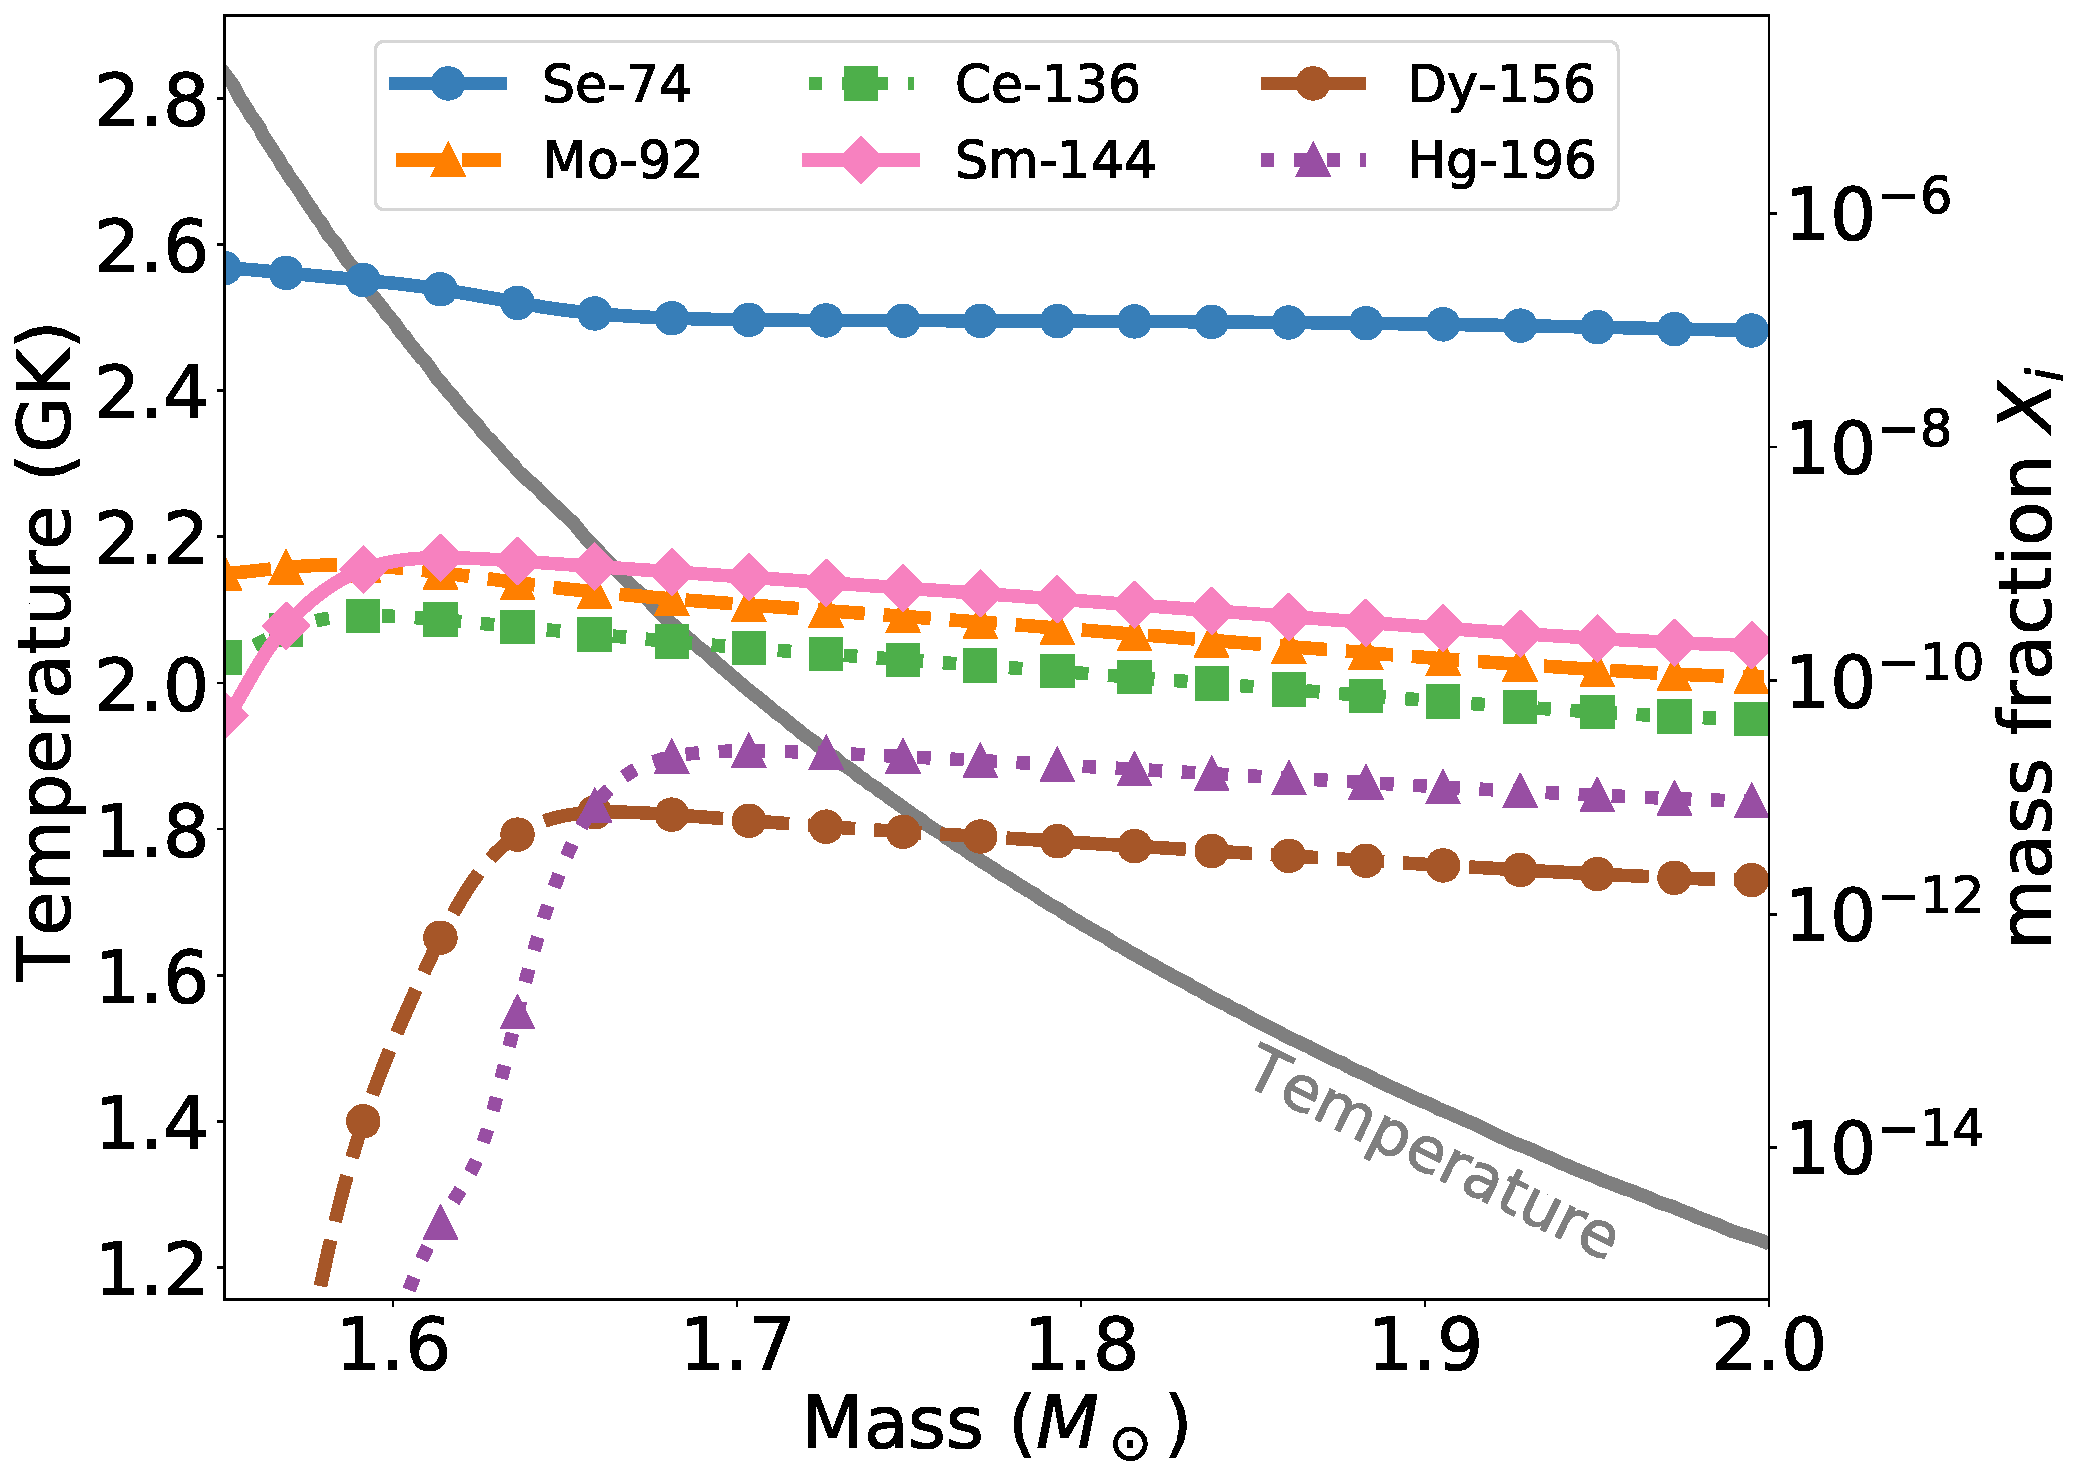
\includegraphics[width=\textwidth]{chapters/2/figures/Temperature_Profile_with_X.pdf}
\caption{Temperature profile and mass fractions after $t=110~\mathrm{sec}$ of ingestion for the MLT mixing scenario. The grey solid line is the temperature, the blue solid line with circles is $^{74}\mathrm{Se}$, the orange dashed line with triangles is $^{92}\mathrm{Mo}$, the green dotted line with squares is $^{136}\mathrm{Ce}$, the pink solid line with diamonds is $^{144}\mathrm{Sm}$, the brown dashed line with cirlces is $^{156}\mathrm{Dy}$, and the purple dotted line with triangles is $^{196}\mathrm{Hg}$.
\label{fig:temperatureprofile}}
\end{figure}

The $\gamma$-process is a temperature dependent phenomena where heavier species are produced at cooler temperatures of $1.5-2~\mathrm{GK}$ and destroyed at hotter temperatures, and the lighter species are produced at hotter temperatures of up to $3.5~\mathrm{GK}$ but not produced at cooler temperatures \citep{rauscherConstrainingAstrophysicalOrigin2013}, but advective flows in this O-shell allow for any given isotope regardless of its mass to be produced at their ideal temperature while still contributing to the nucleosynthesis of lighter species.
Whether an individual isotope will react via $(\gamma,n)$ and $(n,\gamma)$ reactions to continue producing their element or contribute to the production of lighter p-nuclei by  $(\gamma,p)$ and $(\gamma,\alpha)$ reactions is temperature, and therefore mixing speed, dependent.
One result of this is that we can identify locations of peak burning for heavier isotopes where the mass fraction of a species suddenly drops as seen for $^{156}\mathrm{Dy}$, $^{196}\mathrm{Hg}$, and to a lesser extent $^{144}\mathrm{Sm}$.
As explained in the convective H-He shell mergers of \cite{herwigCONVECTIVEREACTIVEPROTON2011}, this is the location where the mixing speed becomes equal to the timescale for reactions.  
This is clearly contrary to what is normally seen in a convective environment where the species are well-mixed with no local features, and to reactive environments where species cannot be replenished because there is limited or no mixing hence why understanding this as a convective-reactive environment is necessary.
Whether a species is advects or reacts can lead to unique nucleosynthetic pathways because heavier species are able to reach hotter temperatures that they would not reach and the products of their reactions can either continue to react in that location or move to another and react with the material there.
Figures \ref{fig:convreacflow1} and \ref{fig:convreacflow2} show example fluxes at the same time and mass number but different mass coordinates.

\begin{figure}[!htbp]
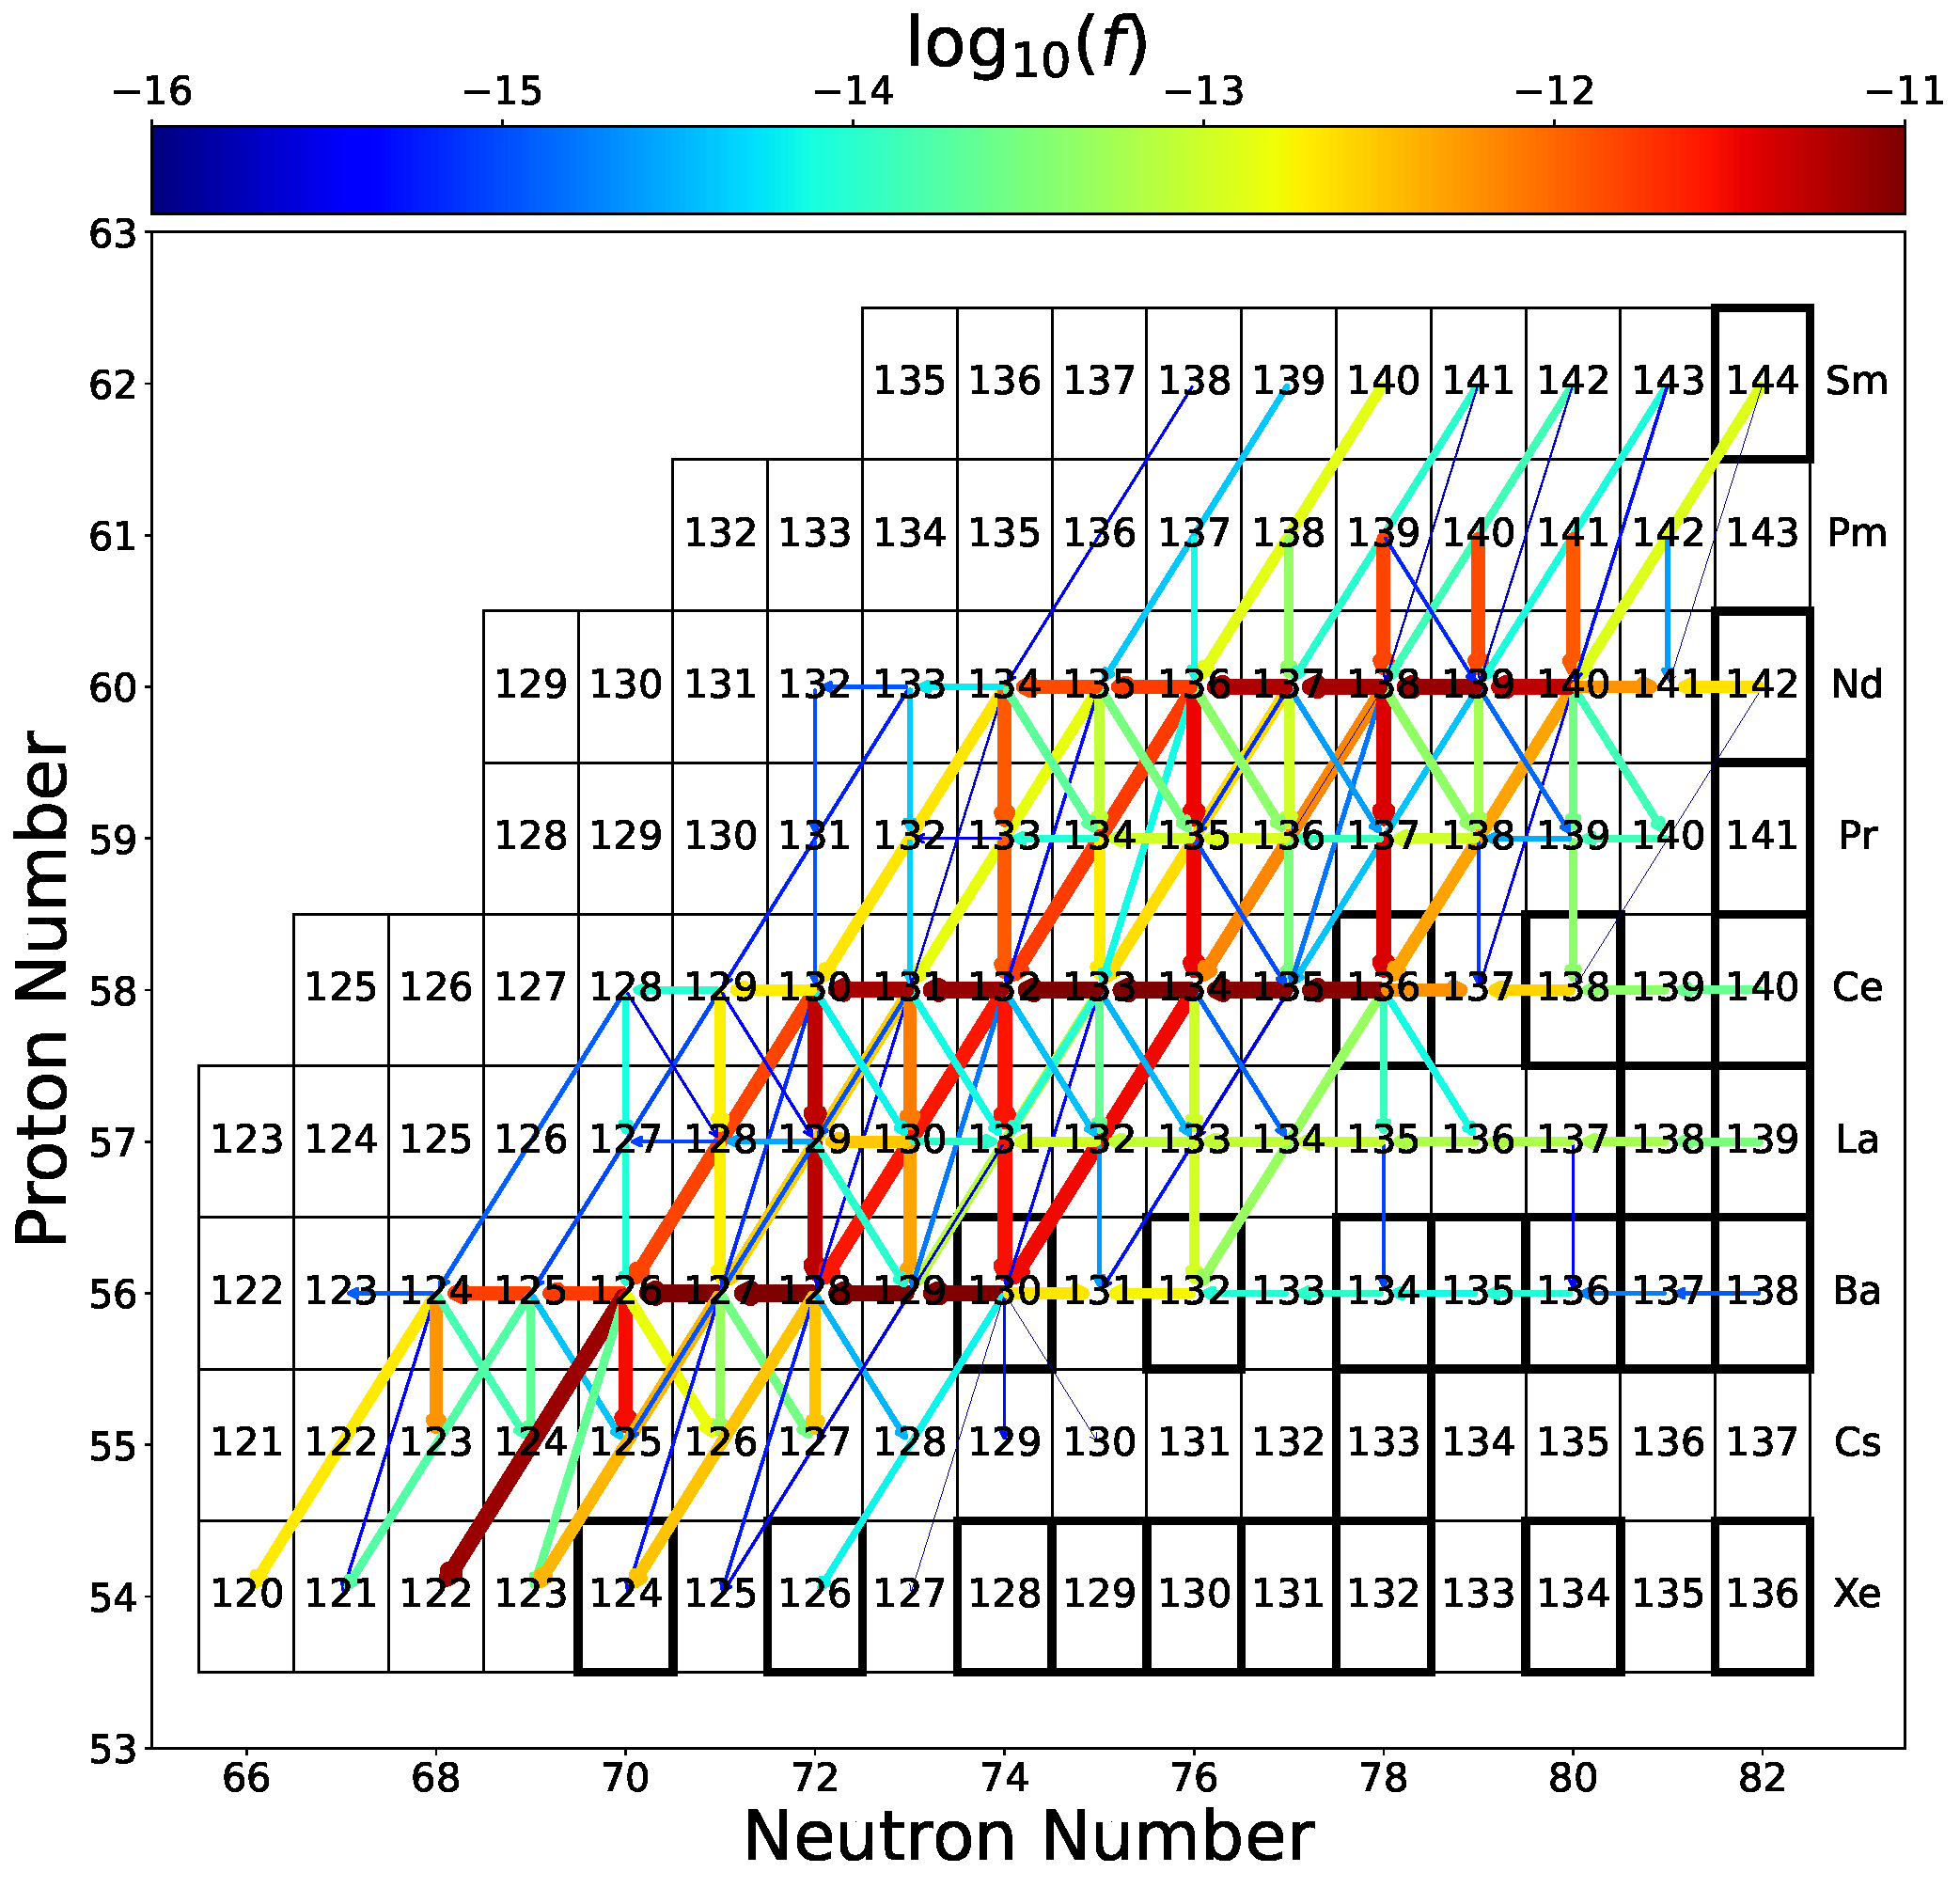
\includegraphics[width=\textwidth]{chapters/2/figures/ce136_network_m1.55551.pdf}
\caption{Nucleosynthetic fluxes $f_{ij}$ at $m=1.55103 M_\odot$ for the MLT scenario for $t=110~\mathrm{sec}$ of ingestion at $2.833~\mathrm{GK}$.
\label{fig:convreacflow1}}
\end{figure}

\begin{figure}[!htbp]
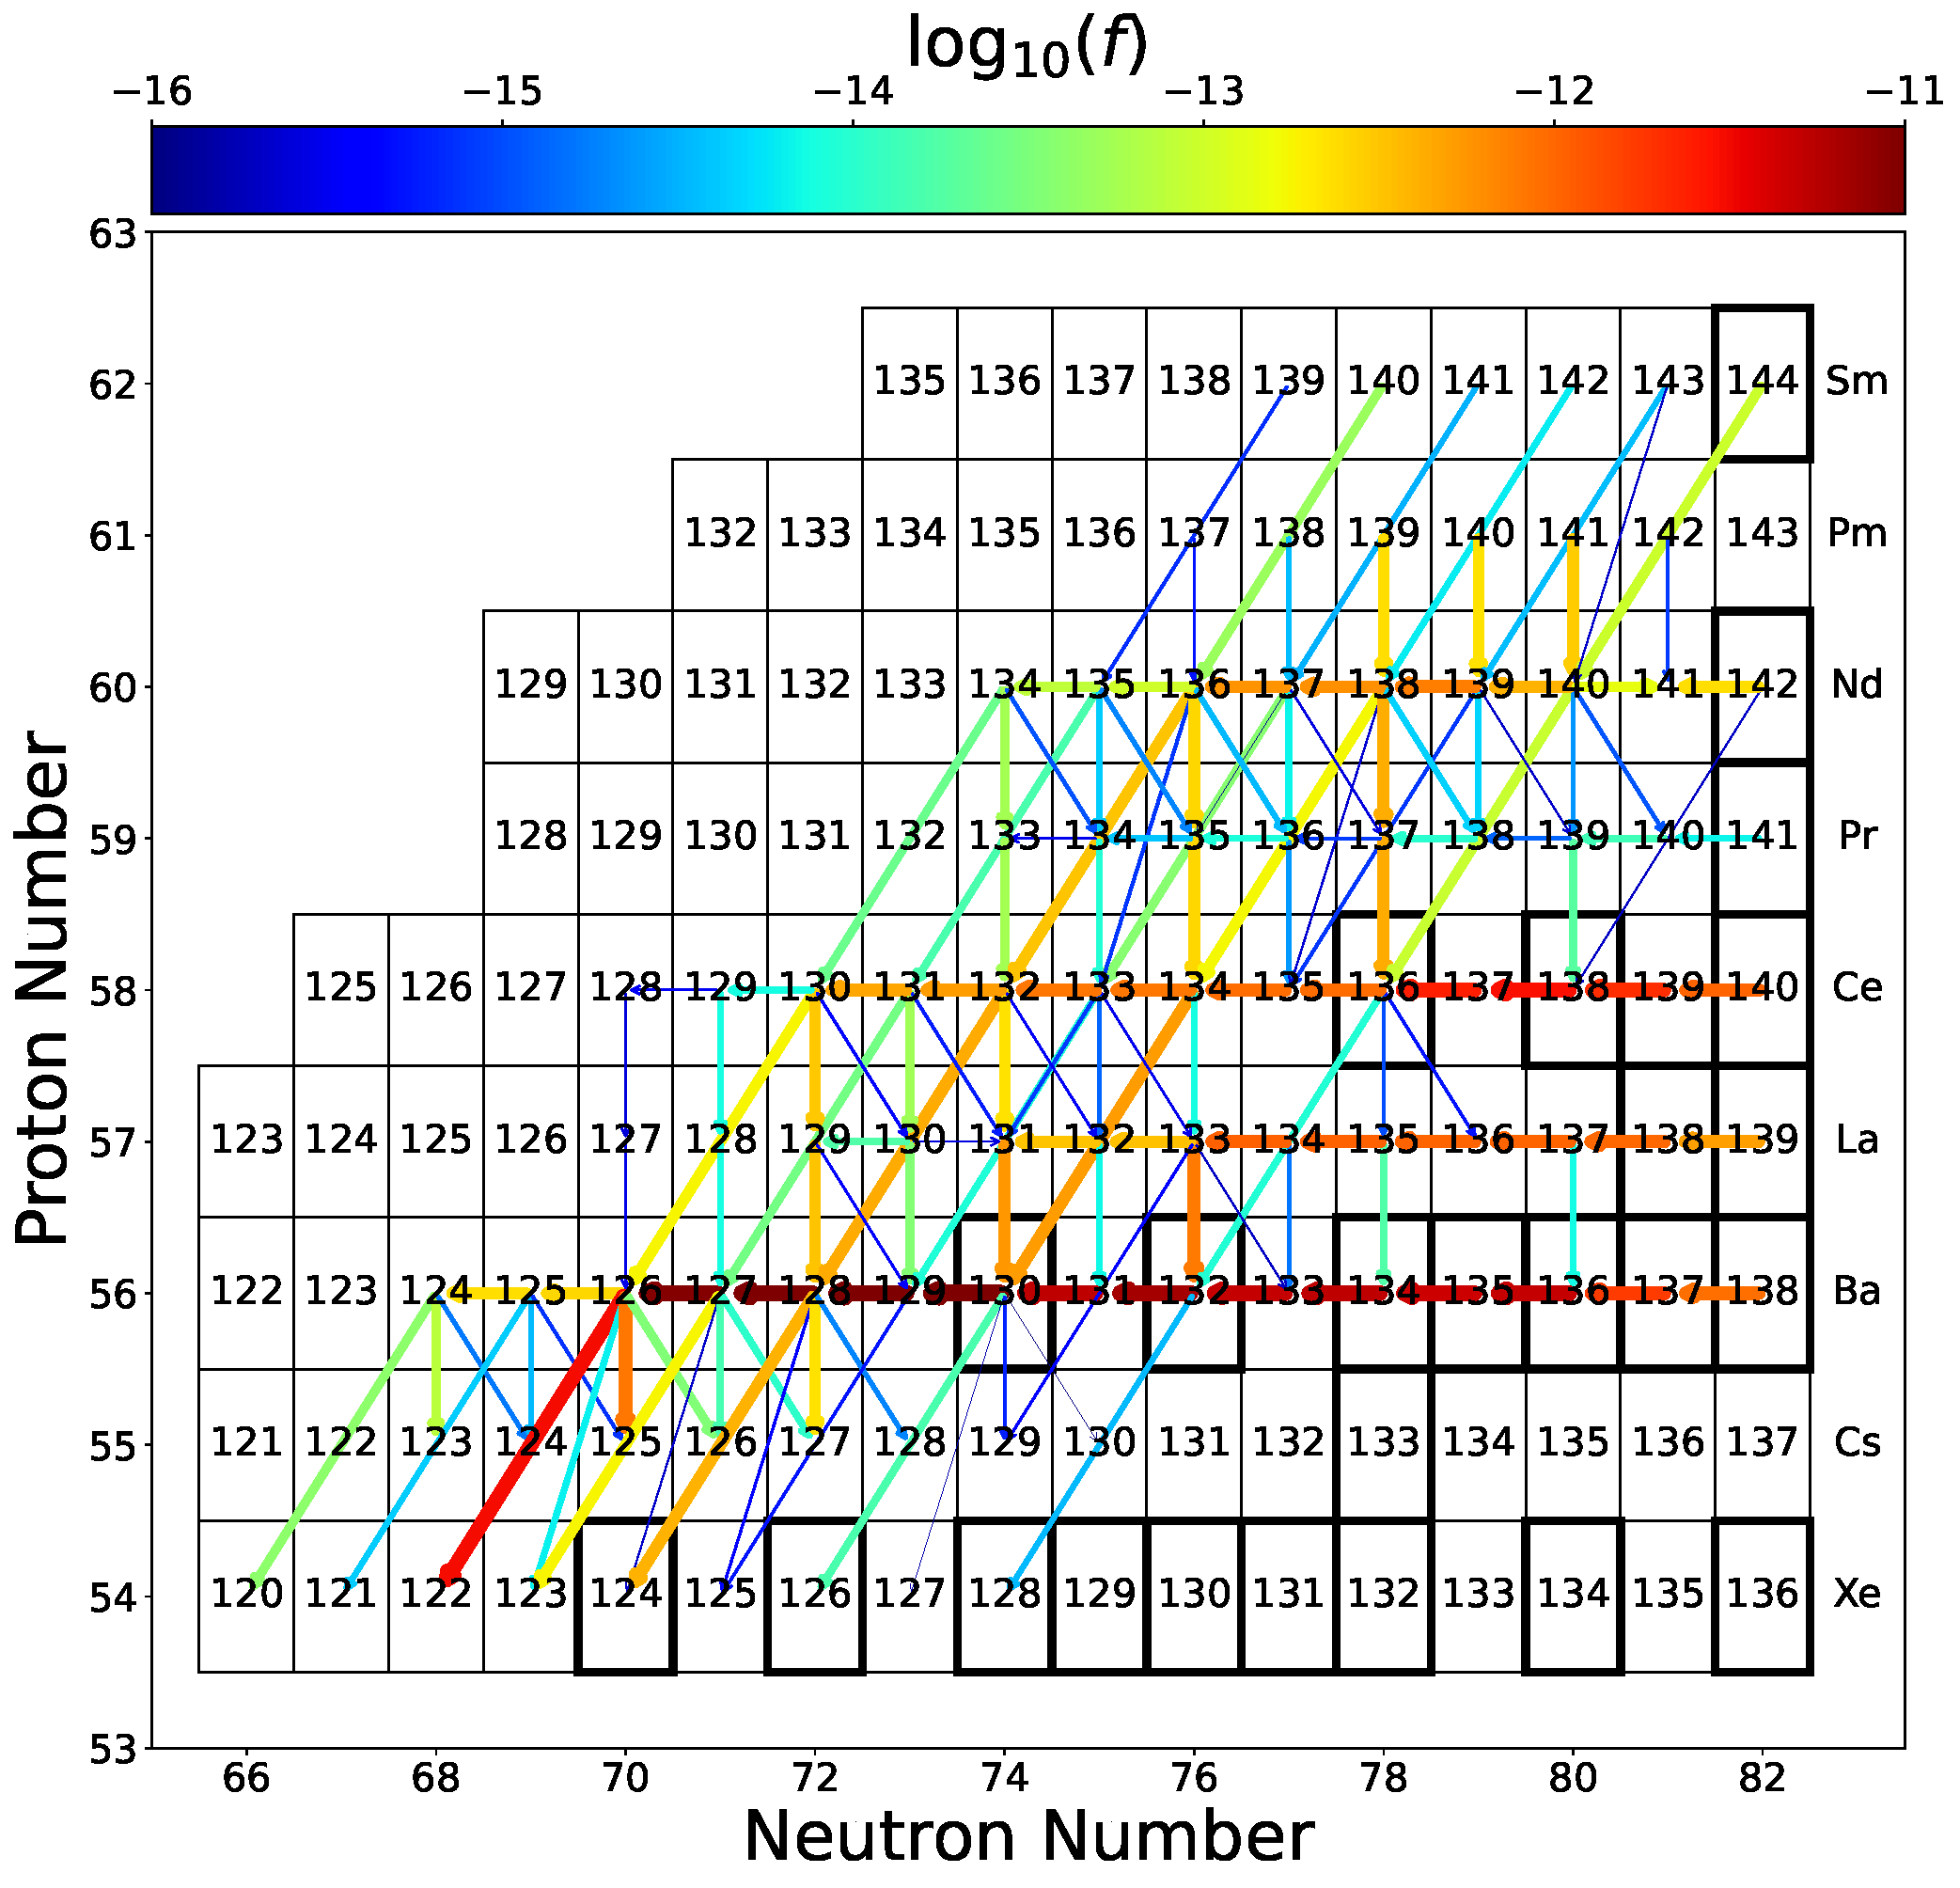
\includegraphics[width=\textwidth]{chapters/2/figures/ce136_network_m1.58017.pdf}
\caption{Nucleosynthetic fluxes $f_{ij}$ at $m=1.58017 M_\odot$ for the MLT scenario for $t=110~\mathrm{sec}$ of ingestion at $2.621~\mathrm{GK}$.
\label{fig:convreacflow2}}
\end{figure}

Fluxes in this shell are not conserved at local mass coordinates because a percentage of a species could be advected to another coordinate.
Figure \ref{fig:convreacflow1} shows $^{136}\mathrm{Ce}$ is net destroyed more efficiently by $^{136}\mathrm{Ce}(\gamma,n)$$^{135}\mathrm{Ce}$ than its production by $^{137}\mathrm{Pr}(\gamma,p)$$^{135}\mathrm{Ce}$, but the mass fraction does not significantly drop as shown in Figure \ref{fig:temperatureprofile} at the bottom of the shell.
This is because it is being produced by $^{137}\mathrm{Ce}(\gamma,n)$$^{136}\mathrm{Ce}$ at a slightly higher position of $m=1.58017M_\odot$ as shown in Figure \ref{fig:convreacflow2} and advected both left and right leading to the peak seen in Figure \ref{fig:temperatureprofile}.
Because $^{136}\mathrm{Ce}$ is being continually replenished by an advective flow, it can continue to produce the unstable Ce isotopes which contribute significant nucleosynthetic fluxes to the production the unstable Ba, La, and Xe isotopes as well as the p-nuclei $^{130}\mathrm{Ba}$ via $^{134}\mathrm{Ce}(\gamma,\alpha)^{130}\mathrm{Ba}$ and $^{132}\mathrm{Ce}(\gamma,p)$$^{131}\mathrm{La}(\gamma,p)$$^{130}\mathrm{Ba}$ at $m=1.55103M_\odot$ in addition to the Ba $(\gamma,n)$ chain at $m=1.58017M_\odot$.
Another feature in the nucleosynthesis is that species are able to co-produce each other.
Although not as strongly shown as it is at other mass coordinates, Figures \ref{fig:convreacflow1} and \ref{fig:convreacflow2} can shown this for $^{136}\mathrm{Ce}$ and $^{137}\mathrm{Ce}$.
$^{137}\mathrm{Ce}$ is both produced by $^{136}\mathrm{Ce}$ and produces it depending on the mass coordinate because of the temperature differences.
Because of the complex relationship between multiple different nucleosynthesis regimes, the exact pathways of production cannot be followed as simply as it could in typical convective or reactive environments.
This raises questions on the impact of seeds as the convective-reactive environment has different $s$-, $i$-, and $r$-seeds present depending on the local mass coordinate.
Figure \ref{fig:temperatureprofile} clearly shows that there is an unequal share of material present as the heaviest seeds are not present at the hottest temperatures and will not be destroyed via $(\gamma,\alpha)$ to the lightest p-nuclei but stop at a certain point, although their products are advected deeper in the shell to the hottest temperatures.
This demonstrates the importance of following how $\gamma$-process nucleosynthesis behaves in this convective-reactive O-shell.

\subsection{Mixing scenario 1: Convective downturns}\label{sec:convdownturnimpact}

3-D hydrodynamic simulations show that the MLT mixing scenario is not accurate for the O-burning shell.
Here we present how the final nucleosynthesis is impacted in the alternative mixing scenario of a convective downturn \citep{jonesIdealizedHydrodynamicSimulations2017} in Figure \ref{fig:impactmixingcases} and will refer to the convective downturn cases as 3D-inspired and their boost factors as done in Figure \ref{fig:all_dconv}.
Across the MLT and all 3-D inspired convective downturn mixing scenarios, there is an average spread in the production of the p-nuclei $0.96~\mathrm{dex}$.

\begin{figure}[!hbt]
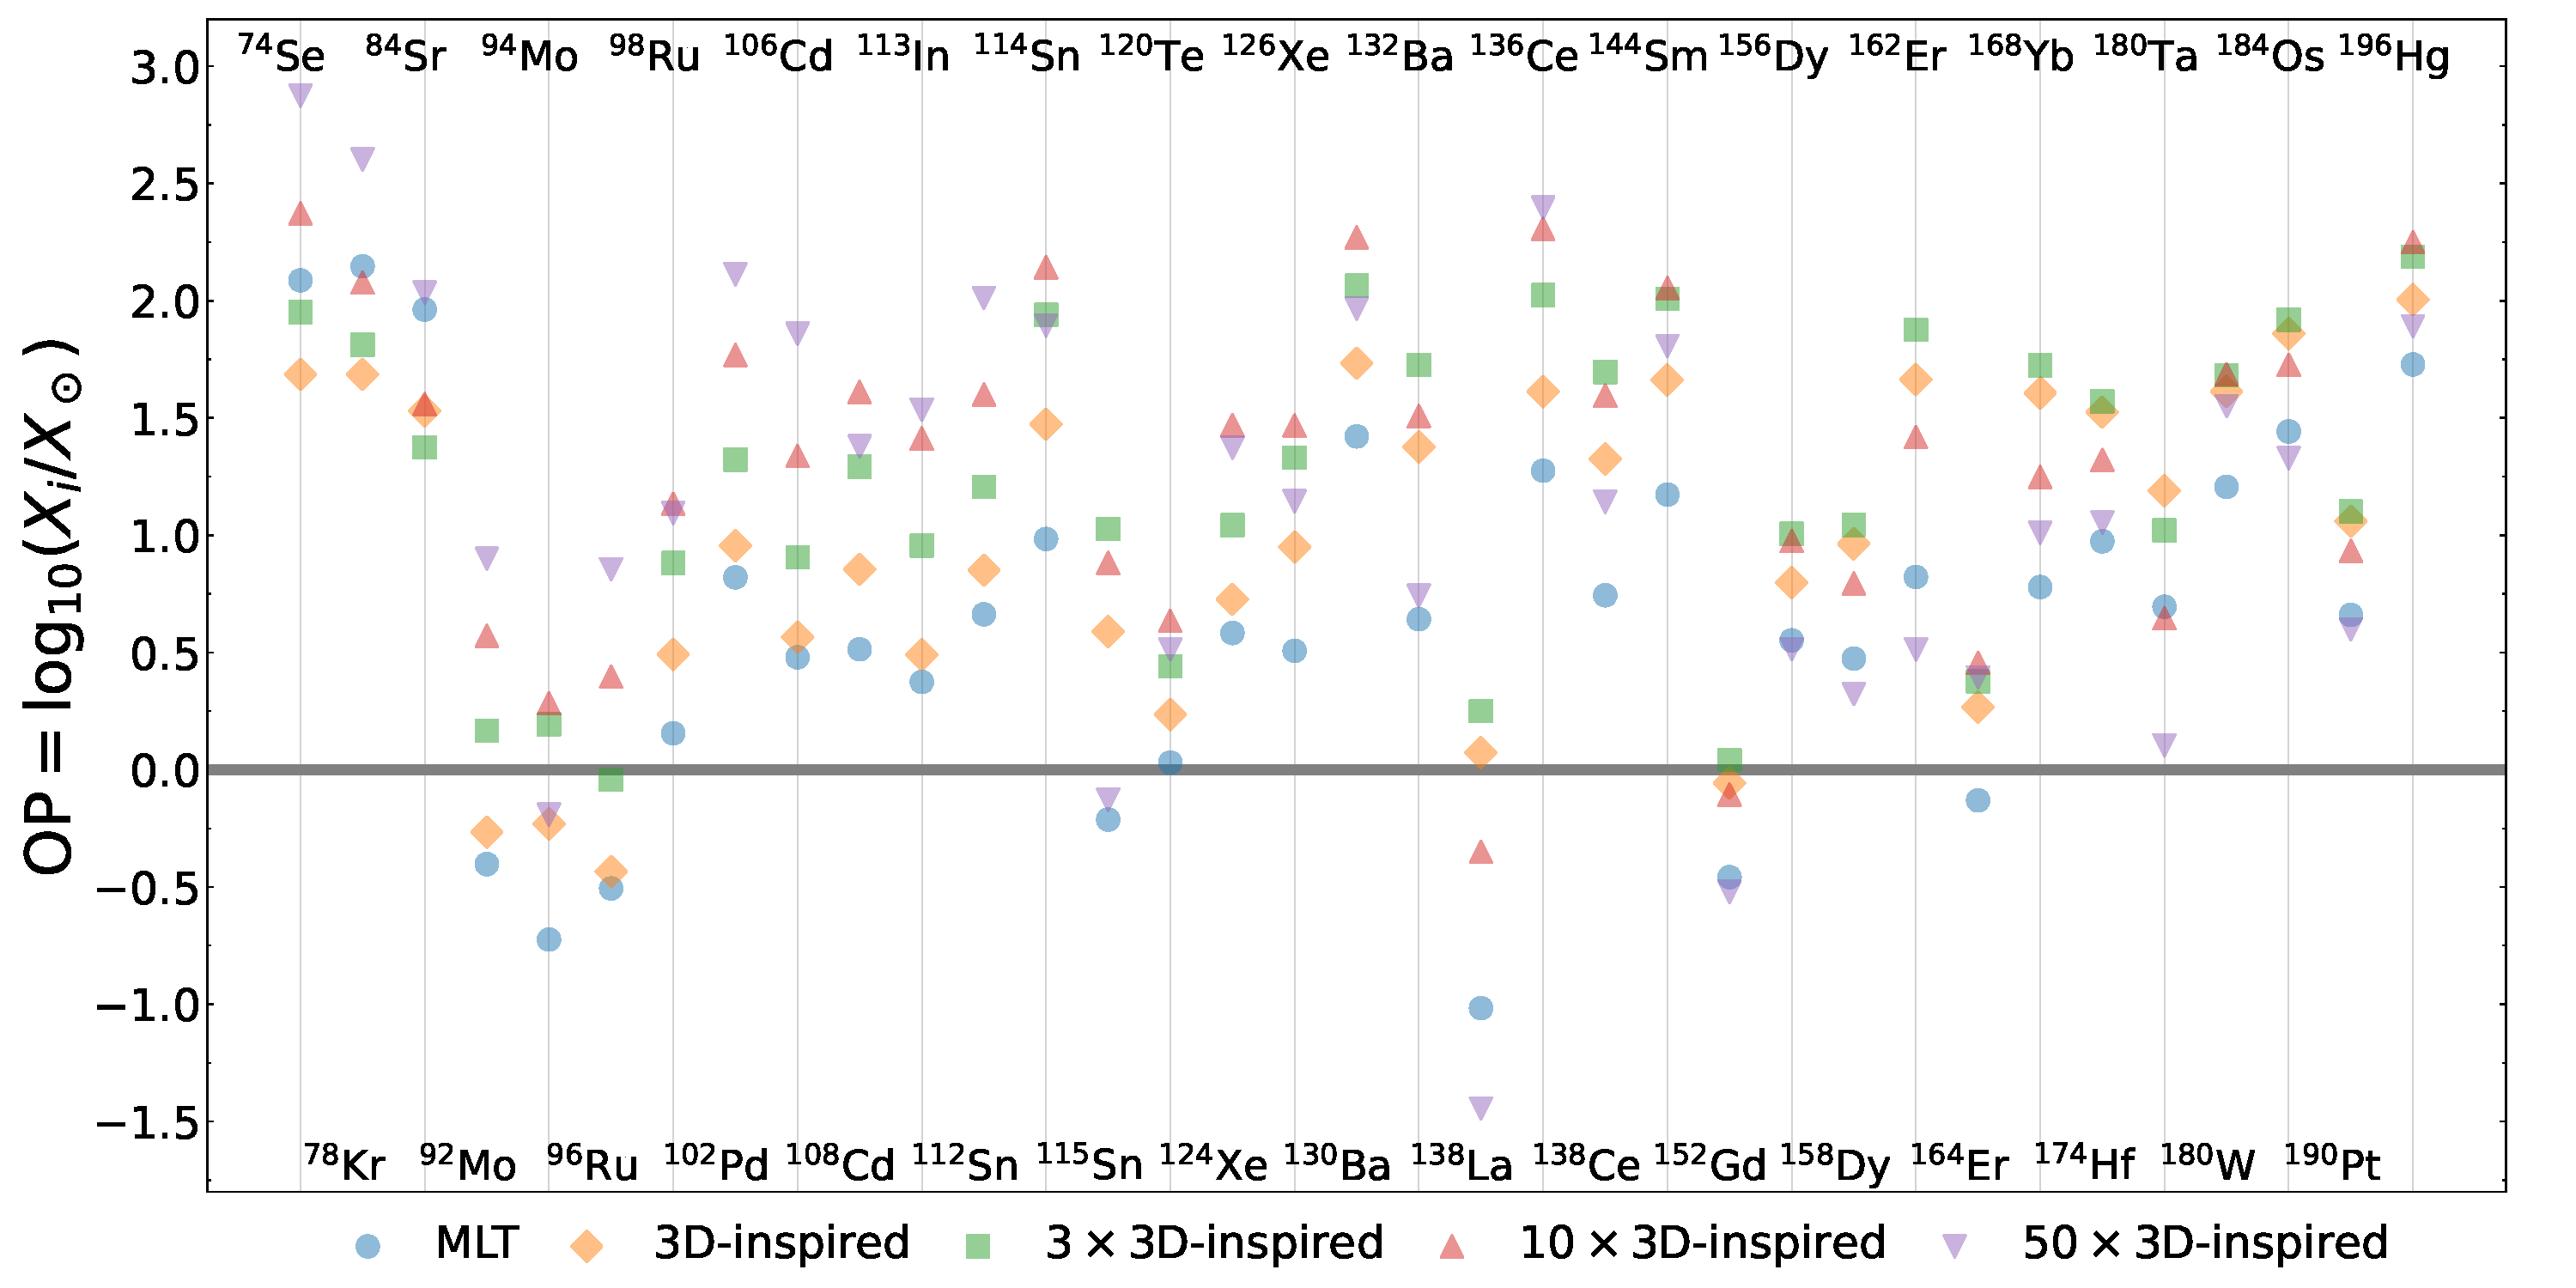
\includegraphics[width=\textwidth]{chapters/2/figures/impact_mixing_cases.pdf}
\caption{The overproduction compared to the solar measurement of the p-nuclei. The blue circle corresponds to the MLT scenario, orange diamond to the 3D-inspired scenario, green square to $3\times$3D-inspired scenario, right side up red triangle to $10\times $3D-inspired, and upside down purple triangle to $50\times$3D-inspired. The thick grey line at $\mathrm{OP}= 0$ corresponds to the solar measurement. The average spread in production is $0.96~\mathrm{dex}$.
\label{fig:impactmixingcases}}
\end{figure}

The presence of a convective downturn increases production globally.
The MLT mixing scenario has an $\mathrm{OP}$ of $0.64~\mathrm{dex}$ and the 3D-inspired scenarios have $0.98~\mathrm{dex}$, $1.23~\mathrm{dex}$, $1.30~\mathrm{dex}$, and $1.12~\mathrm{dex}$ for the $1\times$, $3\times$, $10\times$, $50\times$3D-inspired mixing scenarios respectively. 
Comparing the MLT and $1\times$ cases, all species from $^{92}\mathrm{Mo}$ to $^{196}\mathrm{Hg}$ have their production increased by the appearance of a downturn except the lightest three p-nuclei which are instead decreased.
This is because the mixing speeds at the hottest temperatures are significantly lower, limiting how much of the heavier material is efficiently burned into lighter products.
Local production is not uniformly increased across all the p-nuclei from the downturn. 
For example, comparing the MLT and $1\times$ cases again, $^{168}\mathrm{Yb}$ is increased by $0.83~\mathrm{dex}$ but $^{156}\mathrm{Dy}$ is only increased by $0.25~\mathrm{dex}$.
As the mixing speeds in the 3D-inspired scenario increase, the local and global production changes in a non-linear and non-monotonic way. 
Global production decreases for the $50\times$3D-inspired scenario because the species are now being advected fast enough to the bottom of the O-shell that the decreasing velocities no longer impede production. 
Comparing $^{98}\mathrm{Ru}$ and $^{162}\mathrm{Er}$, both species increase in production as the mixing speed increases, but at the $50\times$ scenario $^{162}\mathrm{Er}$ is decreased by $0.91~\mathrm{dex}$ compared to the $10\times$ scenario whereas $^{98}\mathrm{Ru}$ is produced about the same. 

Another feature that can be seen in Figure \ref{fig:impactmixingcases} is that the ratio of any two isotopic pairs is dependent on the mixing scenario. 
In the $\gamma$-process, isotopes are related by $(\gamma,n)$ and $(\gamma,\alpha)$ reactions which are temperature dependent, and because the mixing speed determines how much of the material will reach a certain temperature it changes whether an element will be destroyed into another.
For the $^{92,94}\mathrm{Mo}$ pair, the MLT, $10\times$, and $50\times$ mixing scenarios $^{92}\mathrm{Mo}$ is more abundant, and in the $1\times$ and $3\times$ scenarios they are nearly equal. 
For the $^{106,108}\mathrm{Cd}$ pair, they are equal for the MLT mixing scenario, and then for all but the $50\times$ scenario $^{108}\mathrm{Cd}$ is more abundant.
Similarly for the $\mathrm{Sn}$ isotopes, $^{114}\mathrm{Sn}$ is more abundant than $^{112}\mathrm{Sn}$ except for the $50\times$3D-inspired mixing scenario.
Not all pairs behave like this, however, as $^{98}\mathrm{Ru}$ and $^{136}\mathrm{Ce}$ are more abundant than $^{96}\mathrm{Ru}$ and $ ^{138}\mathrm{Ce}$.
This demonstrates that the presence of a convective downturn is significant for the production of the p-nuclei. 

\subsection{Mixing scenario 2: Varying the ingestion rate}\label{sec:ingestionimpact}

3-D simulations suggest that entrainment rates of C-shell ashes into the O-shell can be much lower \citep{andrassy3DHydrodynamicSimulations2020}.
Here we present the impact of lowering the rate of ingesting material from the C-shell for the MLT mixing scenario in Figure \ref{fig:ingest_MLT} and the convective downturn scenarios in Figures \ref{fig:ingest_3D}$-$\ref{fig:ingest_50x3D}.

\begin{figure}[!htbp]
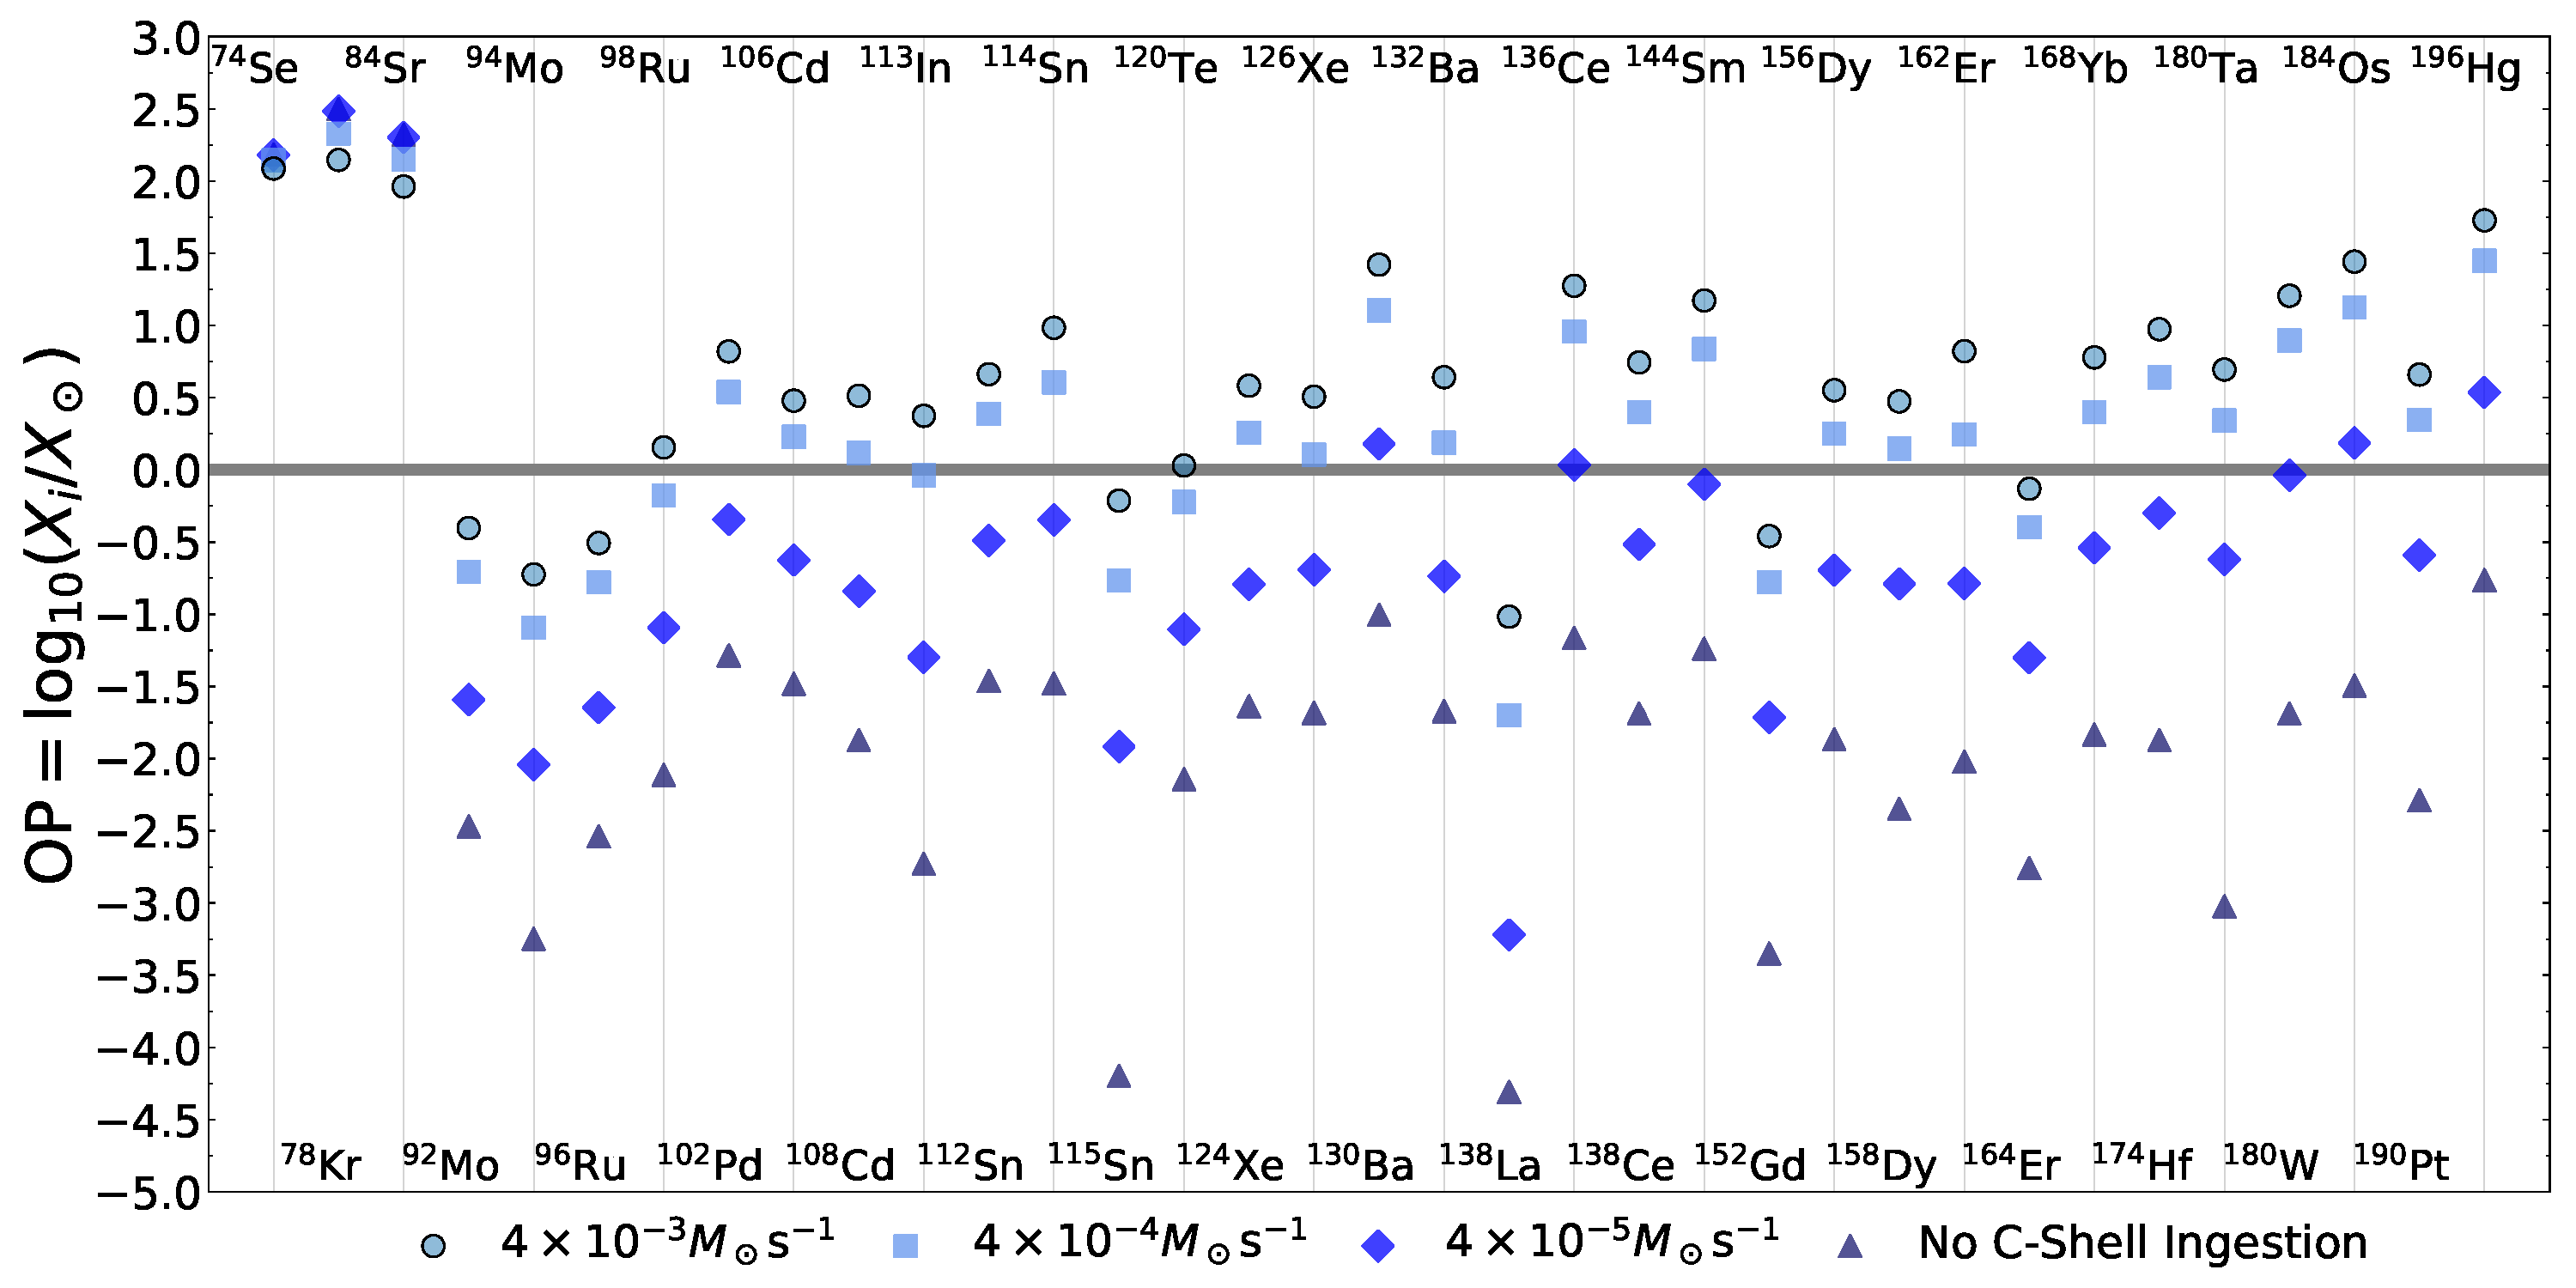
\includegraphics[width=\textwidth]{chapters/2/figures/ingest_MLT.pdf}
\caption{Overproduction compared to solar for the MLT mixing scenario for each ingestion rate. The circle with a black outline corresponds to the base ingestion rate $4\times10^{-3}M_\odot\mathrm{s^{-1}}$, which is the same as the MLT values in Figure \ref{fig:impactmixingcases}. The square corresponds to a rate of $4\times10^{-4}M_\odot\mathrm{s^{-1}}$, the diamond corresponds to a rate of $4\times10^{-5}M_\odot\mathrm{s^{-1}}$, and the triangle corresponds to no ingestion of C-shell material. The thick grey line at $\mathrm{OP}=0$ corresponds to the solar measurement. The average spread in production excluding the no ingestion scenario is $1.22~\mathrm{dex}$.
\label{fig:ingest_MLT}}
\end{figure}

\begin{figure}[!htbp]
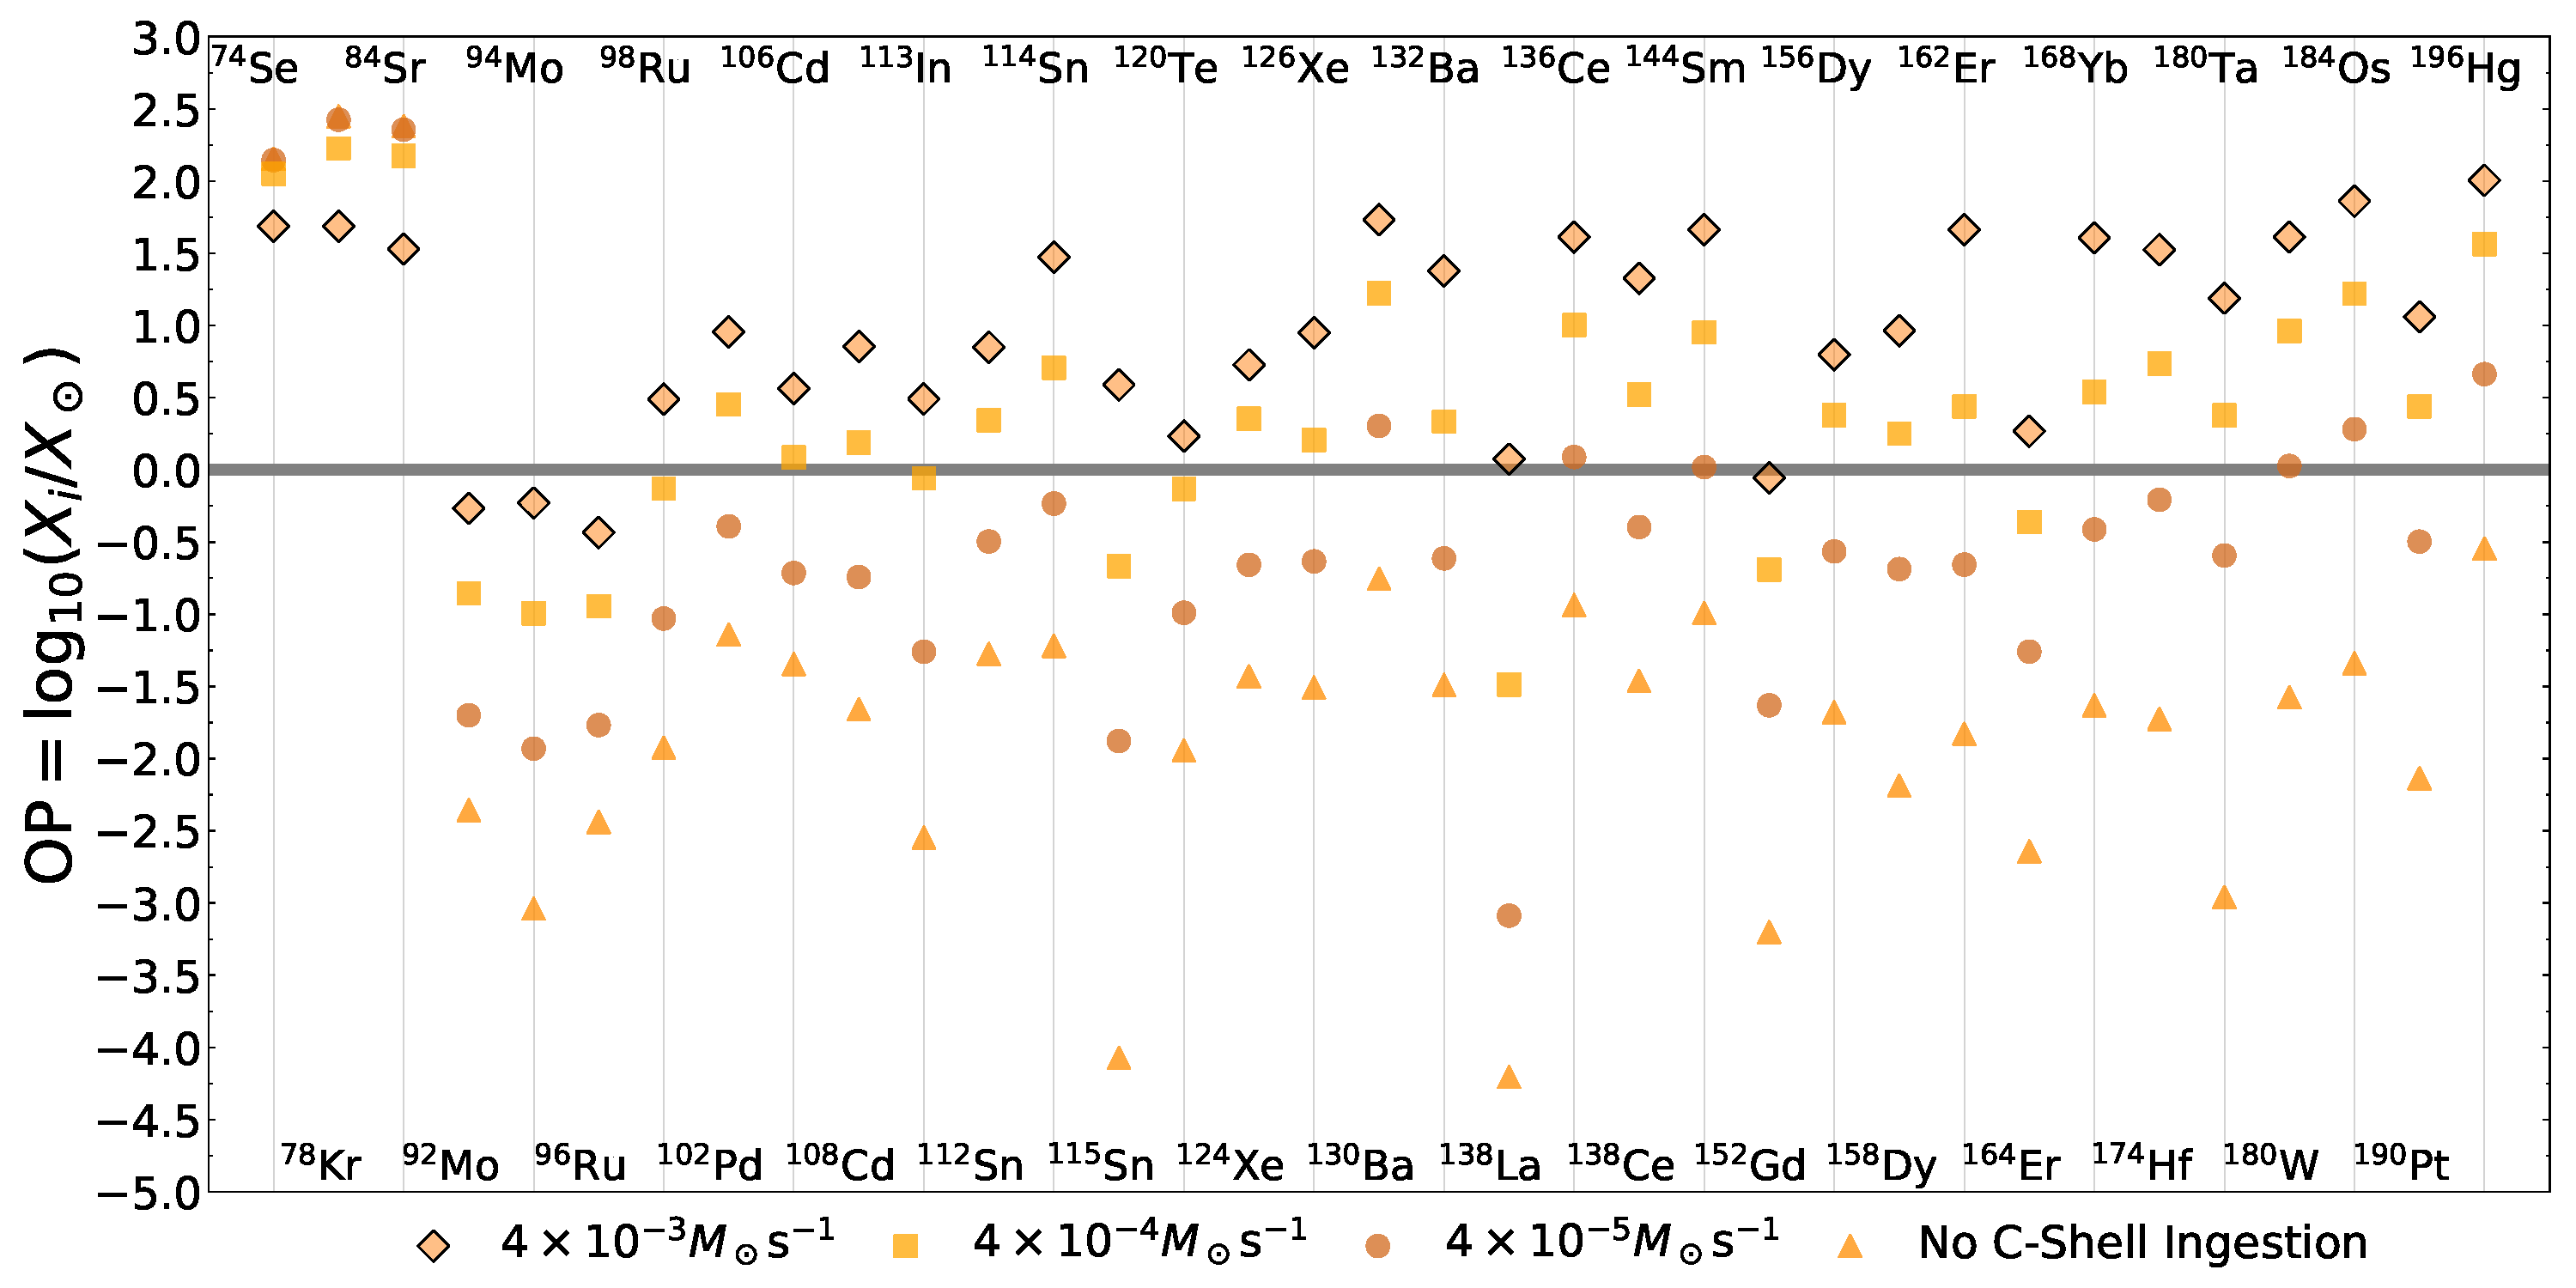
\includegraphics[width=\textwidth]{chapters/2/figures/ingest_3D.pdf}
\caption{Overproduction compared to solar for the 3D-inspired mixing scenario for each ingestion rate. The diamond with a black outline corresponds to the base ingestion rate $4\times10^{-3}M_\odot\mathrm{s^{-1}}$, which is the same as the 3D-inspired values in Figure \ref{fig:impactmixingcases}. The square corresponds to a rate of $4\times10^{-4}M_\odot\mathrm{s^{-1}}$, the circle corresponds to a rate of $4\times10^{-5}M_\odot\mathrm{s^{-1}}$, and the triangle corresponds to no ingestion of C-shell material. The thick grey line at $\mathrm{OP}=0$ corresponds to the solar measurement. The average spread in production excluding the no ingestion scenario is $1.58~\mathrm{dex}$.
\label{fig:ingest_3D}}
\end{figure} 

\begin{figure}[!htbp]
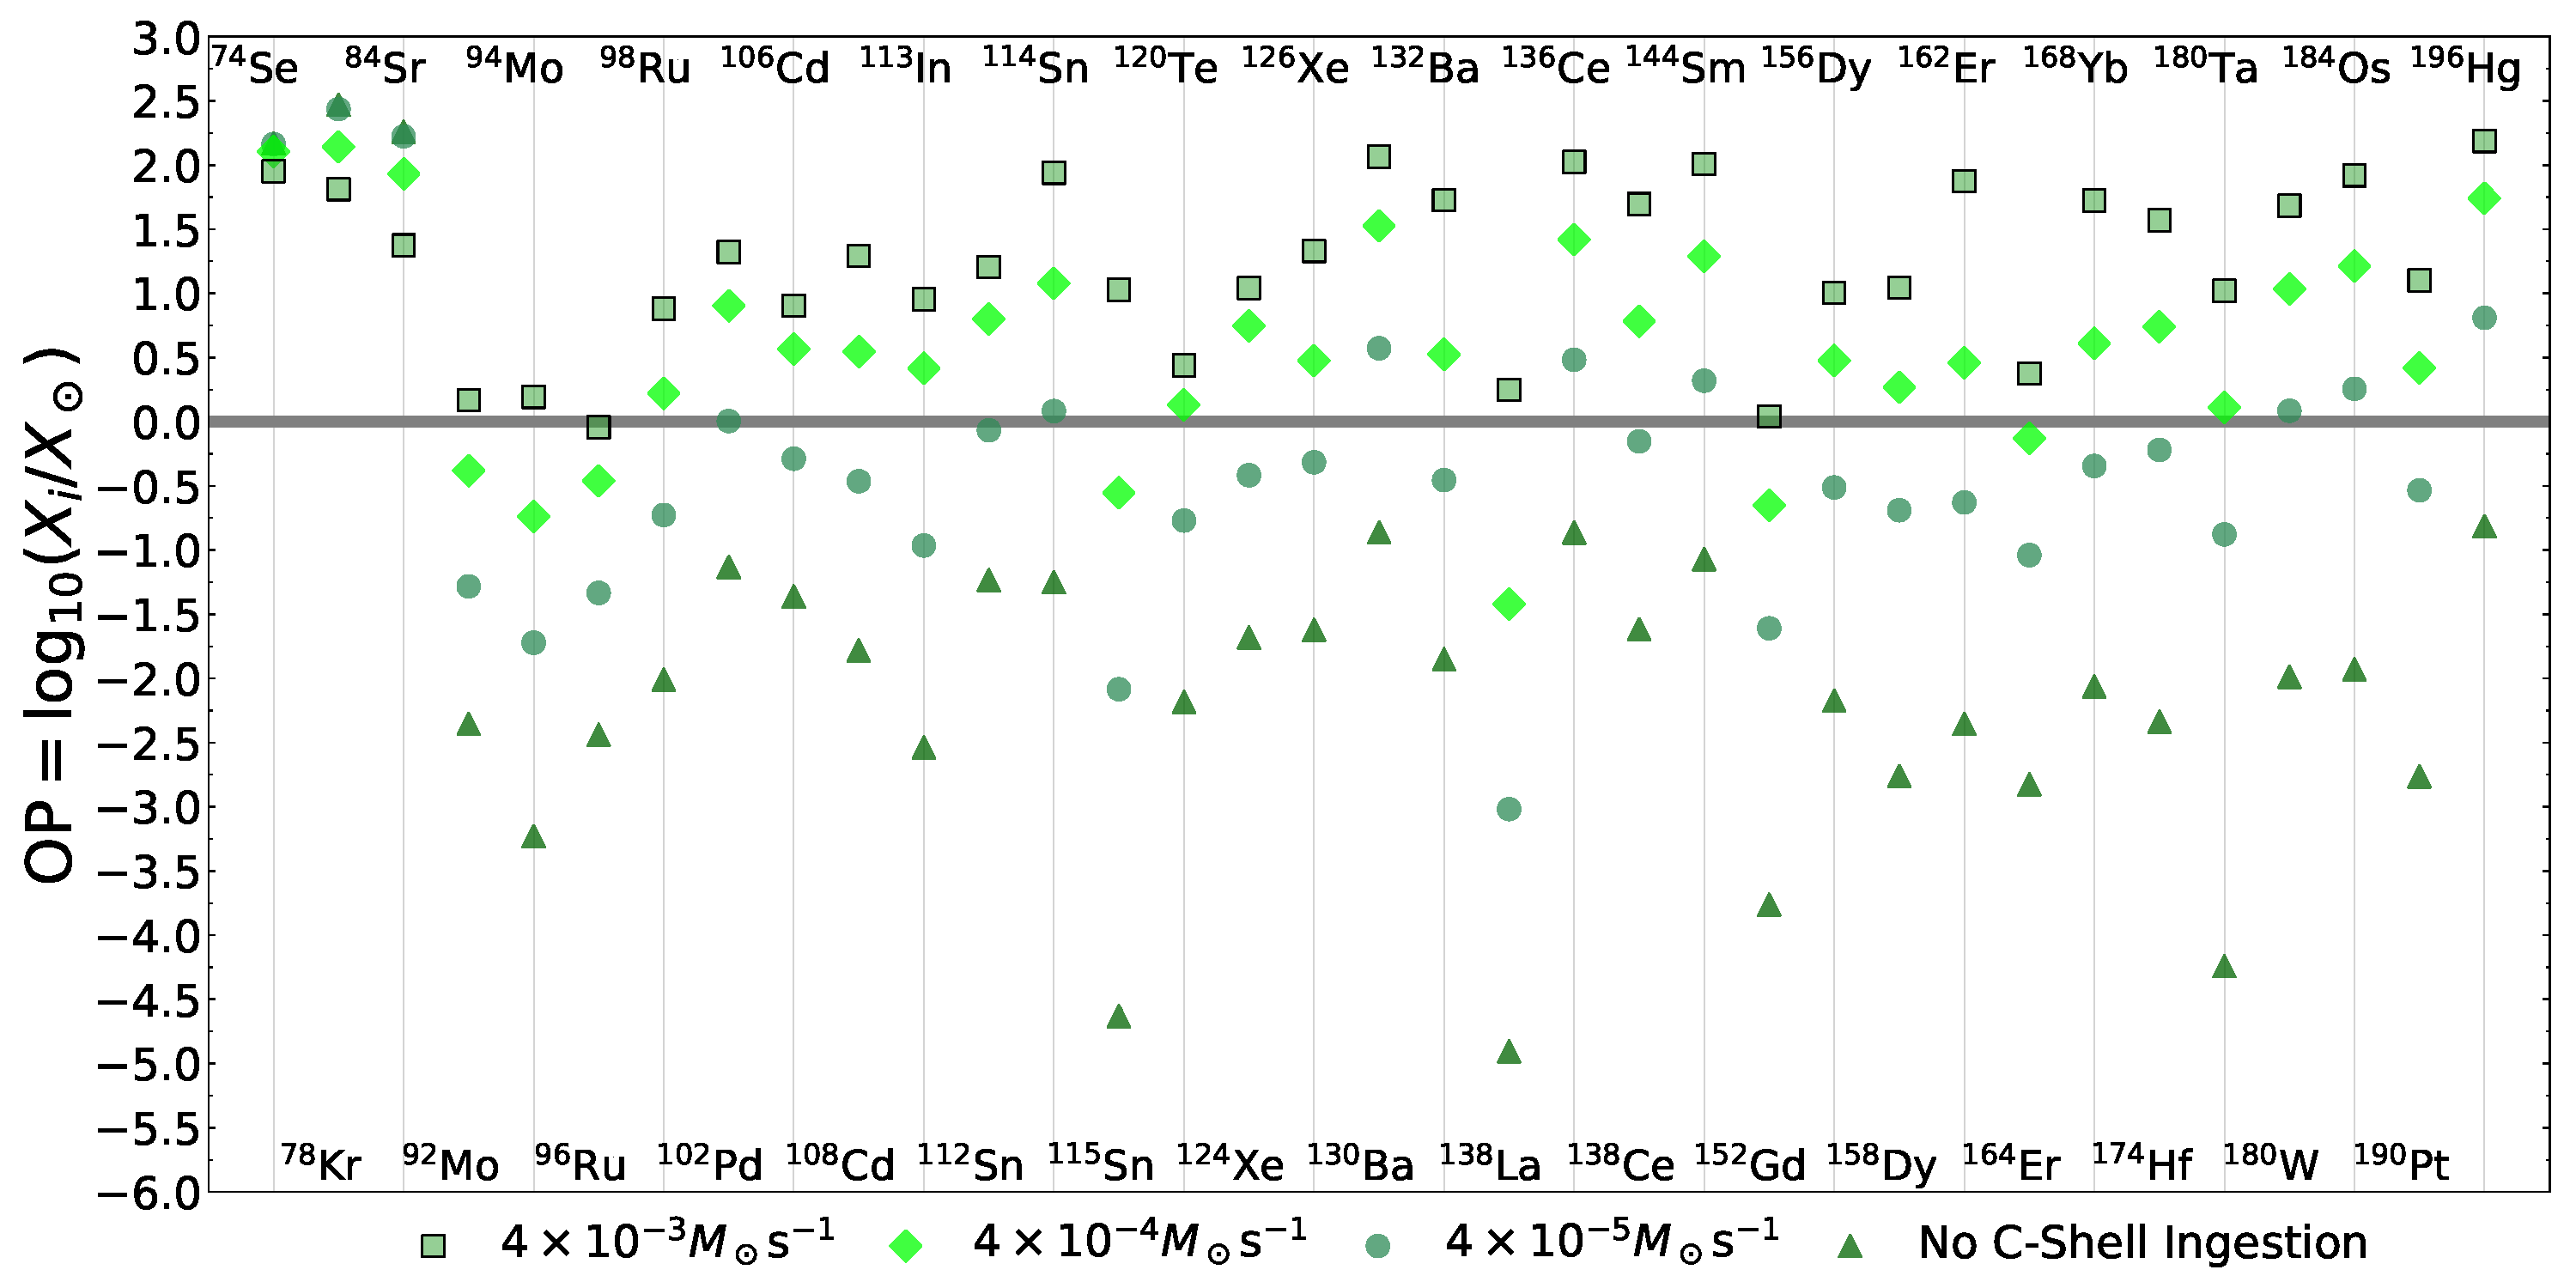
\includegraphics[width=\textwidth]{chapters/2/figures/ingest_3x3D.pdf}
\caption{Overproduction compared to solar for the $3\times$3D-inspired mixing scenario for each ingestion rate. The square with a black outline corresponds to the base ingestion rate $4\times10^{-3}M_\odot\mathrm{s^{-1}}$, which is the same as the $3\times$3D-inspired values in Figure \ref{fig:impactmixingcases}. The diamond corresponds to a rate of $4\times10^{-4}M_\odot\mathrm{s^{-1}}$, the circle corresponds to a rate of $4\times10^{-5}M_\odot\mathrm{s^{-1}}$, and the triangle corresponds to no ingestion of C-shell material. The thick grey line at $\mathrm{OP}=0$ corresponds to the solar measurement. The average spread in production excluding the no ingestion scenario is $1.65~\mathrm{dex}$.
\label{fig:ingest_3x3D}}
\end{figure}

\begin{figure}[!htbp]
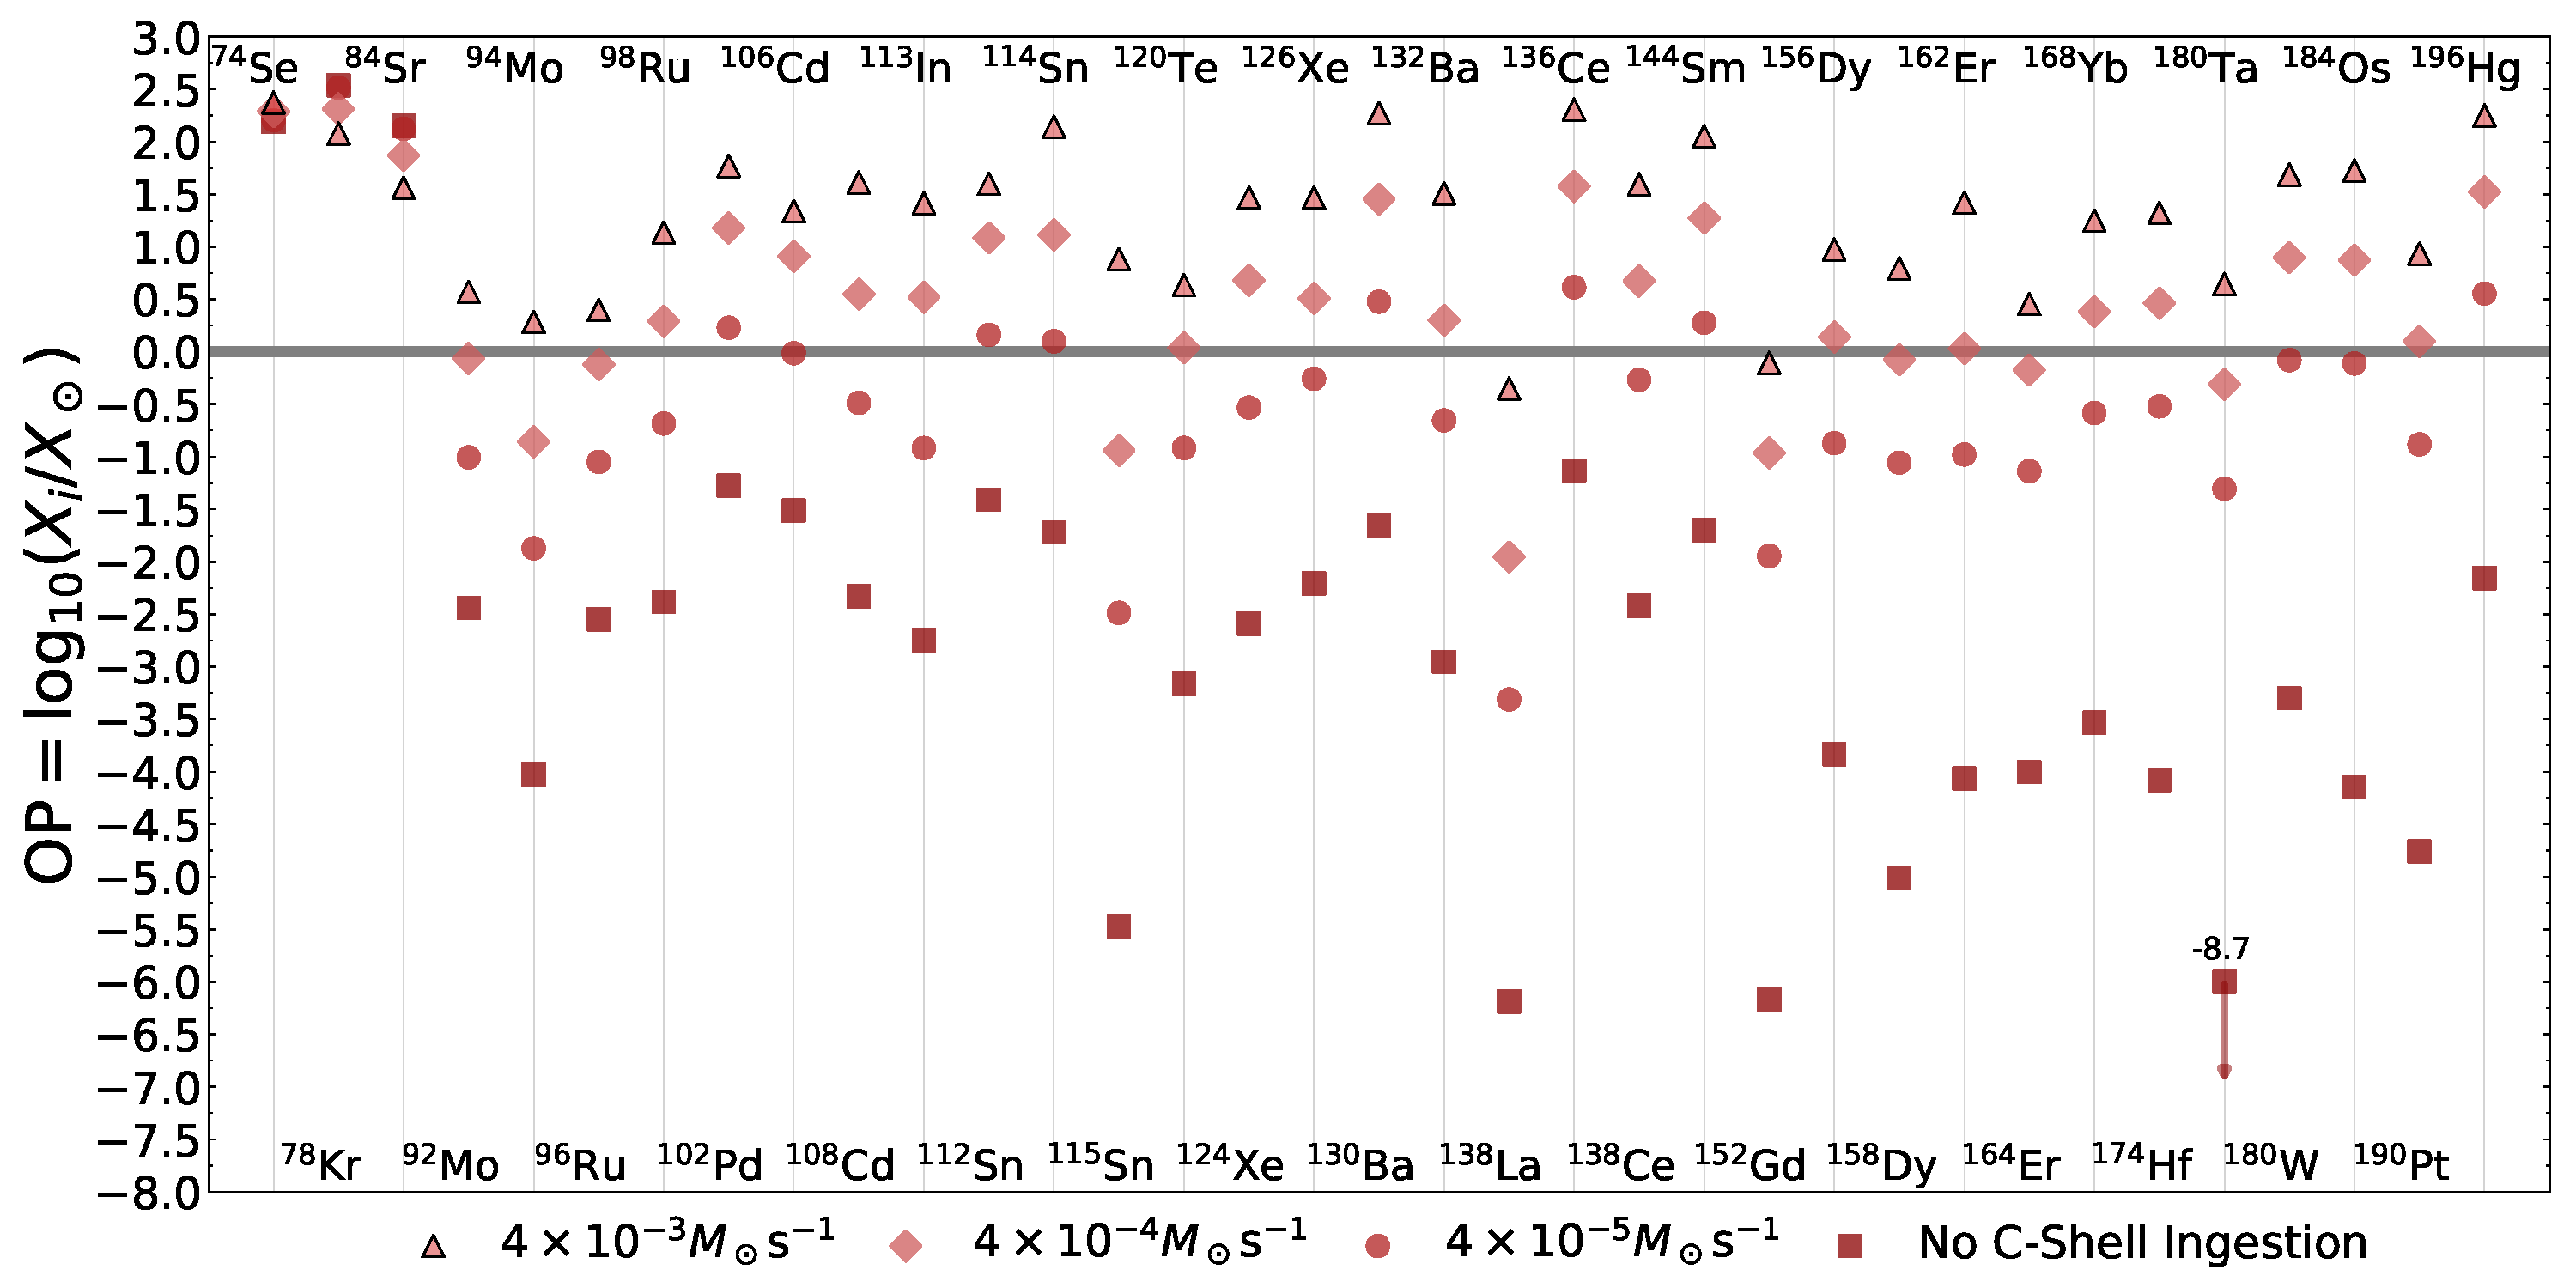
\includegraphics[width=\textwidth]{chapters/2/figures/ingest_10x3D.pdf}
\caption{Overproduction compared to solar for the $10\times$3D-inspired mixing scenario for each ingestion rate. The triangle with a black outline corresponds to the base ingestion rate $4\times10^{-3}M_\odot\mathrm{s^{-1}}$, which is the same as the $10\times$3D-inspired values in Figure \ref{fig:impactmixingcases}. The diamond corresponds to a rate of $4\times10^{-4}M_\odot\mathrm{s^{-1}}$, the circle corresponds to a rate of $4\times10^{-5}M_\odot\mathrm{s^{-1}}$, and the square corresponds to no ingestion of C-shell material. If a point would be plotted out of range, it is denoted with an arrow and its value. The thick grey line at $\mathrm{OP}=0$ corresponds to the solar measurement. The average spread in production excluding the no ingestion scenario is $1.78~\mathrm{dex}$.
\label{fig:ingest_10x3D}} 
\end{figure}

\begin{figure}[!htbp]
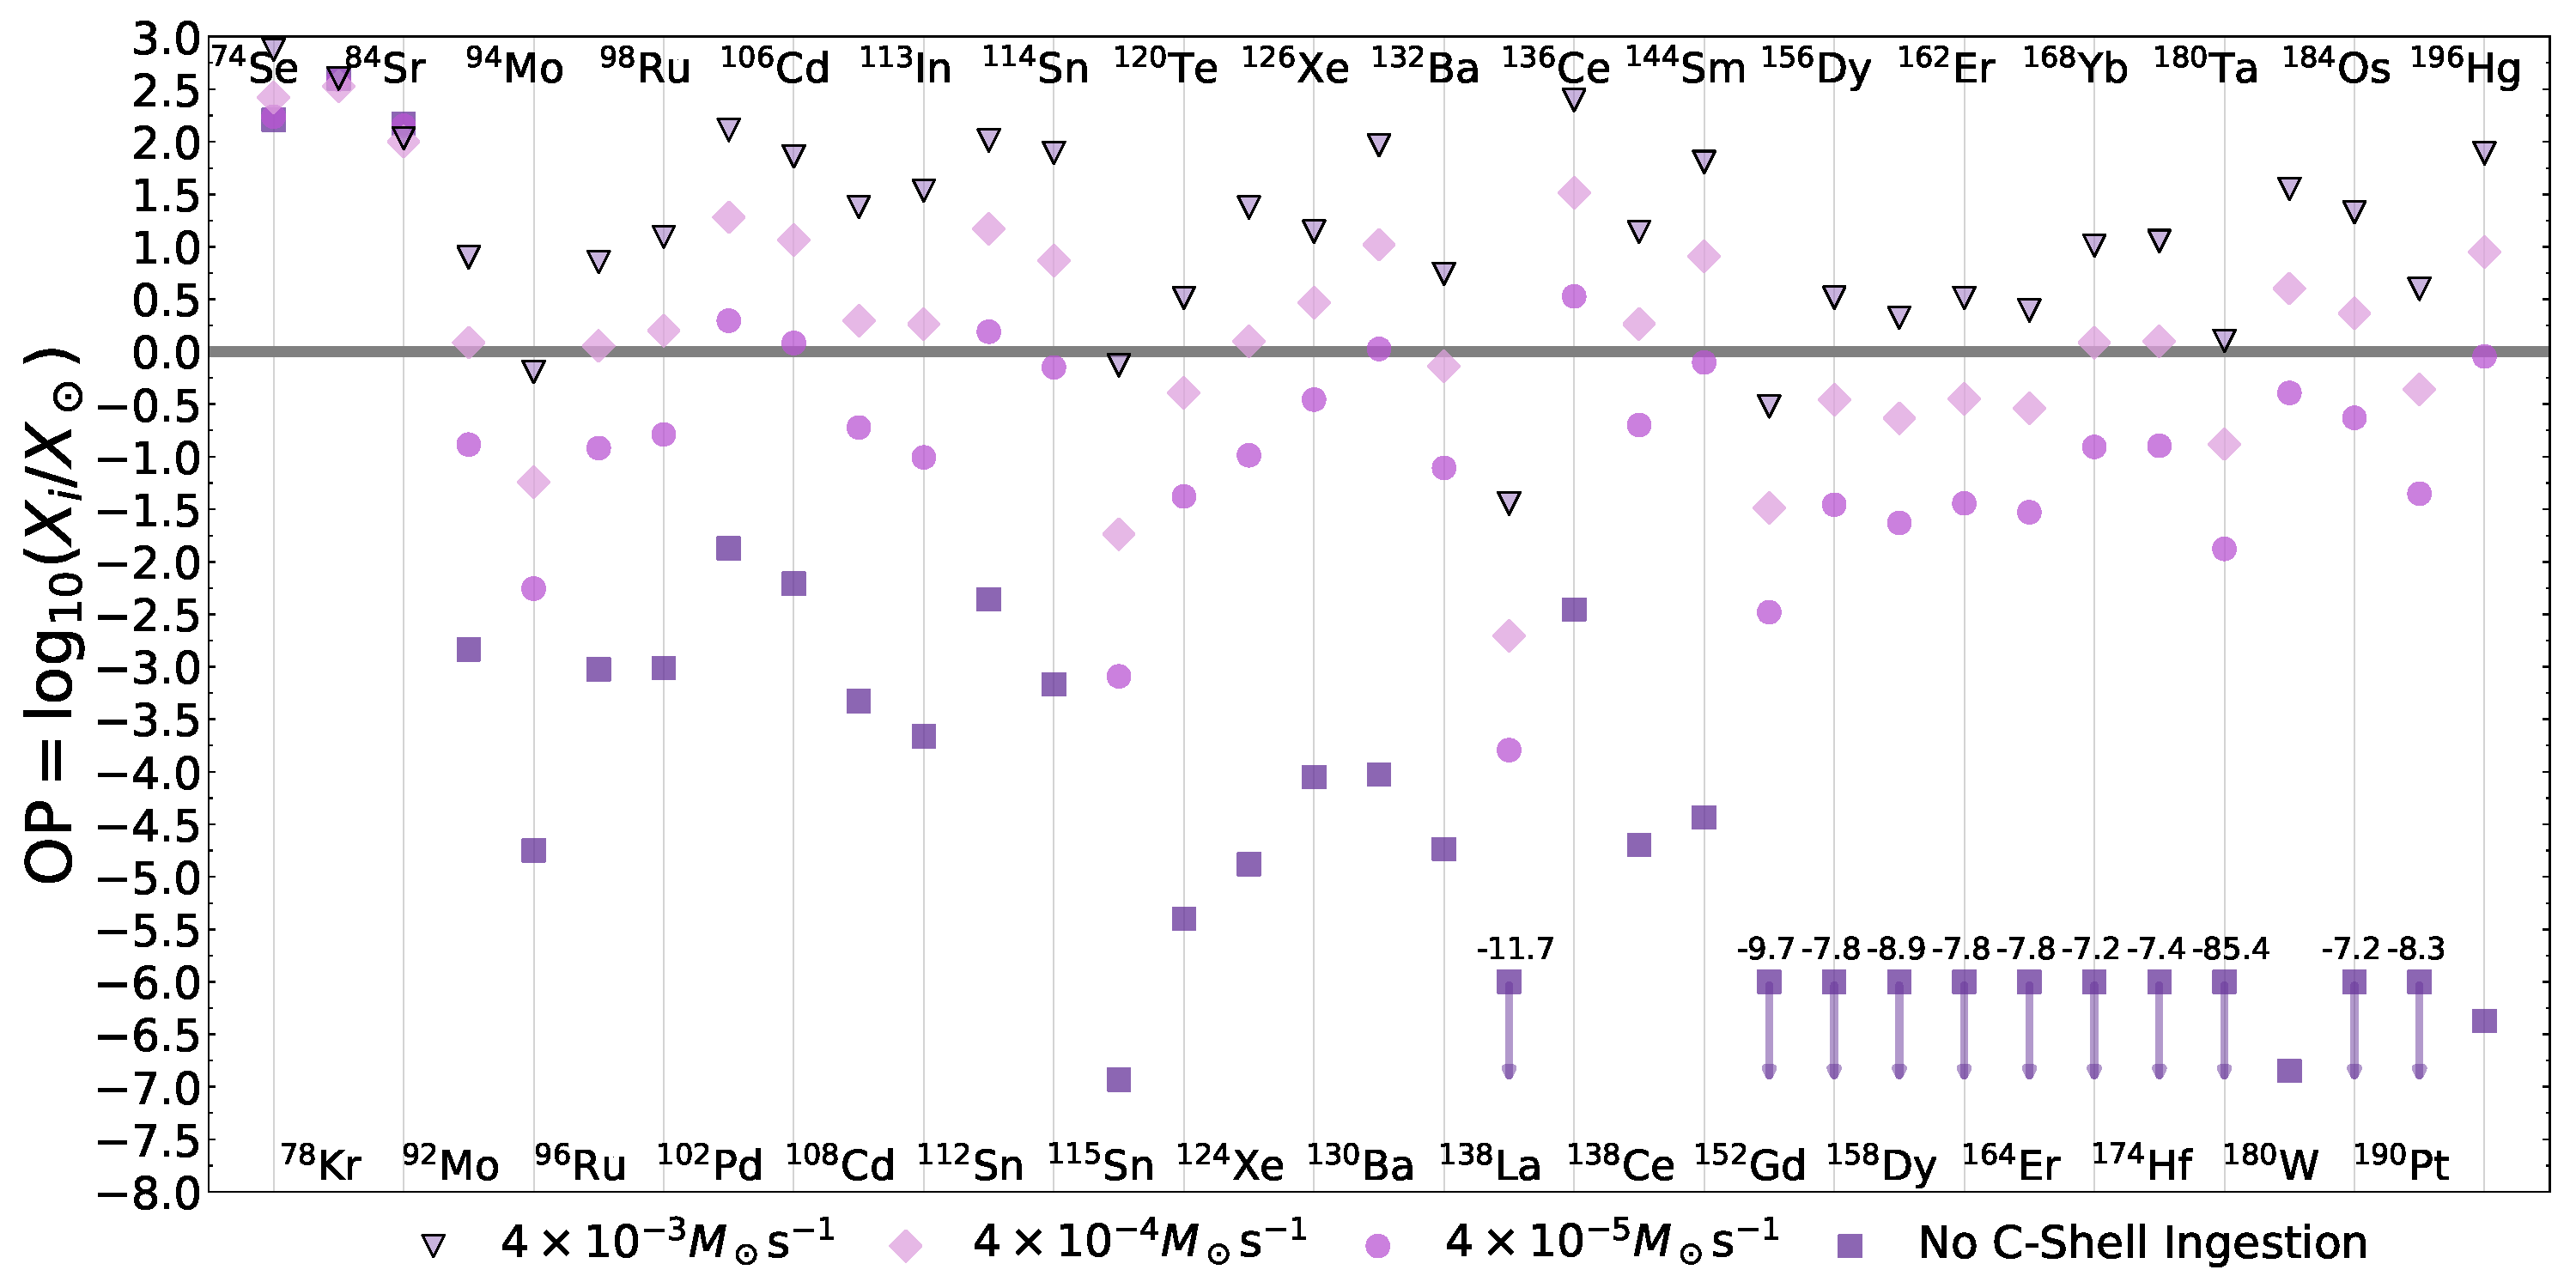
\includegraphics[width=\textwidth]{chapters/2/figures/ingest_50x3D.pdf}
\caption{Overproduction compared to solar for the $50\times$3D-inspired mixing scenario for each ingestion rate. The upside down triangle with a black outline corresponds to the base ingestion rate $4\times10^{-3}M_\odot\mathrm{s^{-1}}$, which is the same as the $50\times$3D-inspired values in Figure \ref{fig:impactmixingcases}. The diamond corresponds to a rate of $4\times10^{-4}M_\odot\mathrm{s^{-1}}$, the circle corresponds to a rate of $4\times10^{-5}M_\odot\mathrm{s^{-1}}$, and the square corresponds to no ingestion of C-shell material. If a point would be plotted out of range, it is denoted with an arrow and its value. The thick grey line at $\mathrm{OP}=0$ corresponds to the solar measurement. The average spread in production excluding the no ingestion scenario is $1.84~\mathrm{dex}$.
\label{fig:ingest_50x3D}}
\end{figure}

The results show how the p-nuclei production is boosted by the ingestion of the C-shell material for all species except $^{74}\mathrm{Se}$, $^{78}\mathrm{Kr}$, and $^{84}\mathrm{Sr}$.
These three isotopes decrease with ingestion rate because they are net destroyed during the O-C shell merger as the hottest temperature $\gamma$-process temperatures are not reached in this shell as Figure \ref{fig:temperatureprofile} shows.
All other isotopes have a boost in their production in a similar way for all isotopes with an increase in ingestion rate, and demonstrate diminishing returns as ingestion rate increase.
Additionally, the convective downturn cases have significant underproductions of $^{115}\mathrm{Sn}$, $^{138}\mathrm{La}$, $^{152}\mathrm{Gd}$, and $^{180}\mathrm{Ta}$.
For the $10$ and $50$ boost factor cases all p-nuclei $A\geq115$ are underproduced and $A\geq152$ are dramatically underproduced.
This shows how the presence of an O-C shell merger is necessary for pre-explosive $\gamma$-process to dominate the production of the p-nuclei.
Across the MLT and convective dowturn cases the average spread in production of cases with C-shell ingestion are $1.22$, $1.58$, $1.65$, $1.78$, and $1.84~\mathrm{dex}$.
This global spread in production grows with mixing speed shows the importance of the mixing speeds.
Across ingestion rate the pattern of the isotopes and ratios between pairs are generally preserved, although this is not always the case as shown with the $\mathrm{Sn}$ isotopes for the $50\times$ convective downturn scenario.
This demonstrates the importance of the O-C shell merger and the impacts of ingestion rate on the production of the p-nuclei.

\subsection{Mixing scenario 3: Convective dips from GOSH-like feedback and a partial merger}\label{sec:goshimpact}

O-C shell mergers experience non-radial, spherically asymmetric instabilities like GOSHs due to energy feedbacks \citep{andrassy3DHydrodynamicSimulations2020} and could experience dips in the convective profile.
Here we present the impact on the final production of p-nuclei from considering a dip in the convectivce profile from a GOSH-like event and a partial merger in Figure \ref{fig:impactmixingcases_GOSH_partial}.
The impact of the GOSH-like and the partial merger scenarios impact the production of the p-nuclei in a very similar way for all isotopes with the exceptions of $^{74}\mathrm{Se}$, $^{78}\mathrm{Kr}$, $^{84}\mathrm{Sr}$, and $^{180}\mathrm{Ta}$. 
The GOSH-like and deeper GOSH-like mixing scenarios have an average $\mathrm{OP}$ of $0.47~\mathrm{dex}$ and $0.18~\mathrm{dex}$, and the partial merger and deeper partial merger mixing scenarios have an average $\mathrm{OP}$ of $0.54~\mathrm{dex}$ and $0.31~\mathrm{dex}$.

\begin{figure}[!htbp]
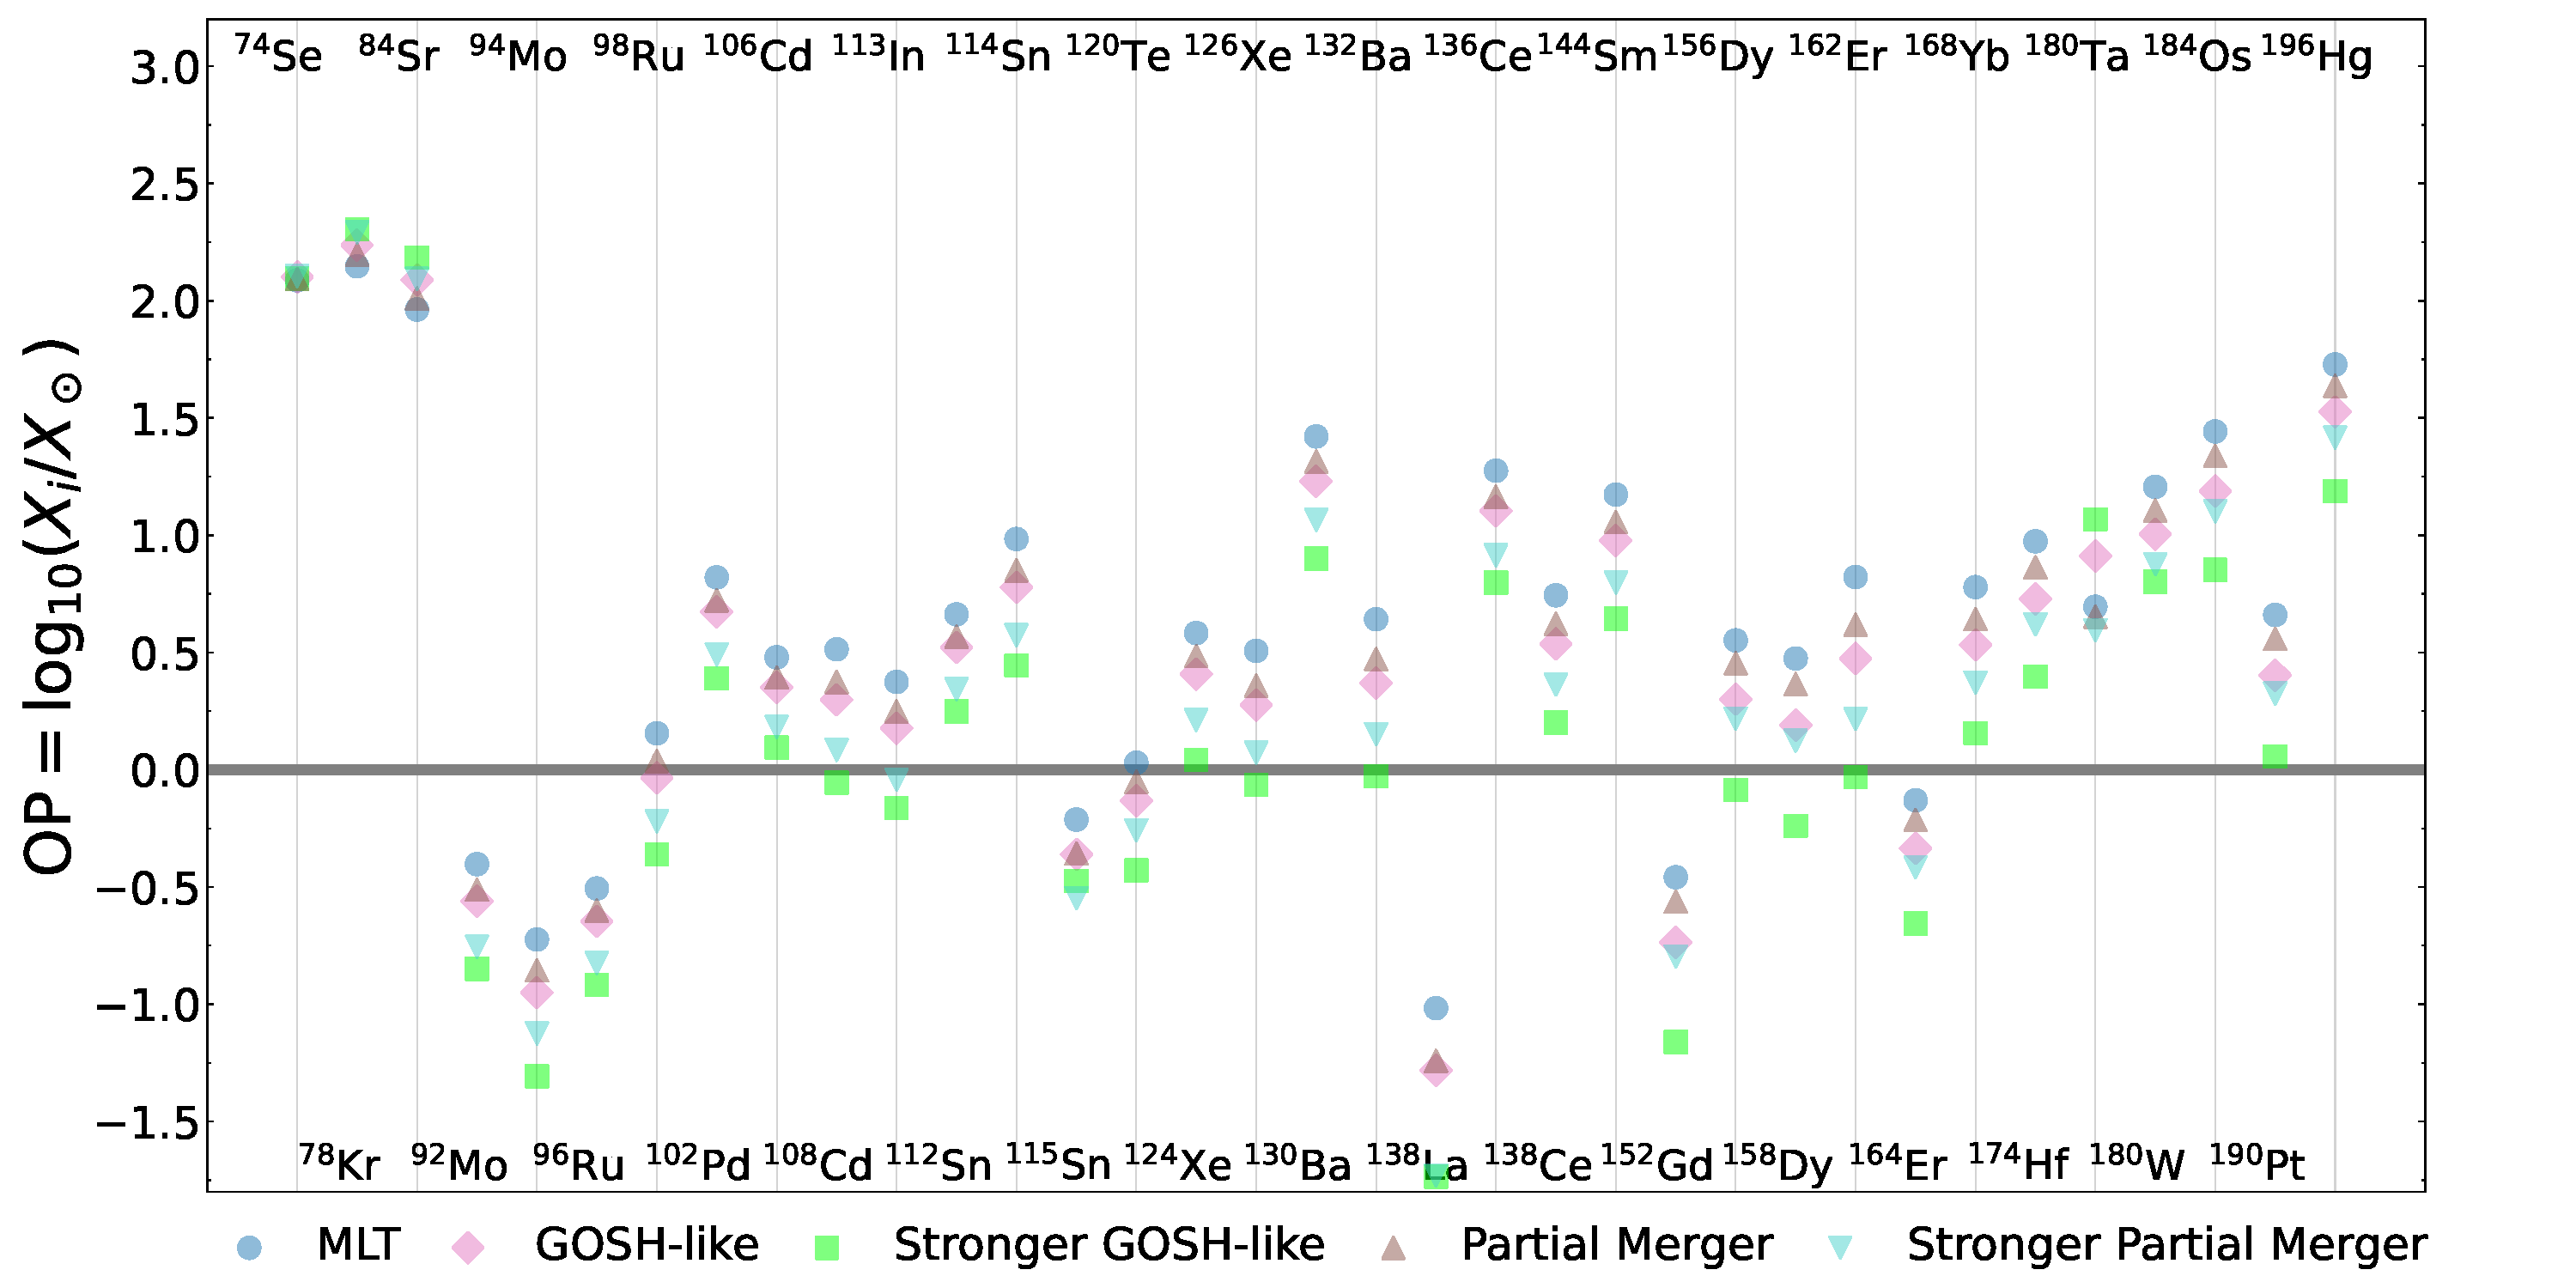
\includegraphics[width=\textwidth]{chapters/2/figures/impact_mixing_GOSH_partial.pdf}
\caption{The overproduction of all p-nuclei with respect to the solar amount. The blue circle corresponds to the MLT scenario, pink diamond to GOSH-like scenario, lime square to deeper GOSH-like scenario, right side up brown triangle to partial merger scenario, and upside down turquoise triangle to deeper partial merger scenario. The thick grey line at $\mathrm{OP} = 0$ corresponds to the solar measurement. The average spread in production is $0.51~\mathrm{dex}$.
\label{fig:impactmixingcases_GOSH_partial}}
\end{figure}

The three lightest p-nuclei are not produced efficiently in the O-shell as discussed above and are significantly less impacted than by convective downturn as the velocities in the relevant nucleosynthetic region are not as impacted.
$^{180}\mathrm{Ta}$ has its production boosted by the introduction of the GOSH-like mixing scenarios compared to the MLT and partial merger scenarios which have roughly equal production.
The other p-nuclei behave nearly uniformly in response to the dip in convective velocities.
The dip decreases the production of the p-nuclei compared to the baseline MLT mixing scenario. 
The partial merger serves as a barrier for the ingested C-shell material to efficiently travel into the region, and the GOSH-like dip interrupts the convective-reactive nature of the environment.
This is also the reason why the global production drops for the scenarios with deeper dips. 
They also show a preference for the location of the dip as production with the partial merger is higher than the GOSH-like scenario.
Preventing the movement of species deeper in the O-shell where its hot enough to undergo photo-disintegration directly inhibits its ability to undergo convective-reactive nucleosynthesis and therefore decreases production more than slowly down the flow of seeds.
The dip is also why $^{78}\mathrm{Kr}$ and $^{84}\mathrm{Sr}$ show slight increases, as the material that would advect up to colder temperatures are impeded.
The pattern of the p-nuclei and ratio between isotopes is also generally preserved across these mixing scenarios.
This demonstrates the importance of whether there is a dip in the convective velocities and the location of that dip as it could decrease production.

\subsection{Nuclear physics impact and mixing dependencies}\label{sec:nuclearimpact}

The timescales of nuclear reactions play a key role in the convective-reactive O-shell and as shown above the relevance of a nuclear reaction depends on the mixing speeds.
We present the results of varying the input nuclear physics for the MLT mixing scenario in Figure \ref{fig:nuclearimpact_MLT} and Table \ref{tab:mlt_corr} and the convective downturn mixing scenarios in Figures \ref{fig:nuclearimpact_3D}$-$\ref{fig:nuclearimpact_50x3D} and Tables \ref{tab:3d_corr}$-$\ref{tab:50x3d_corr}.

\begin{figure}
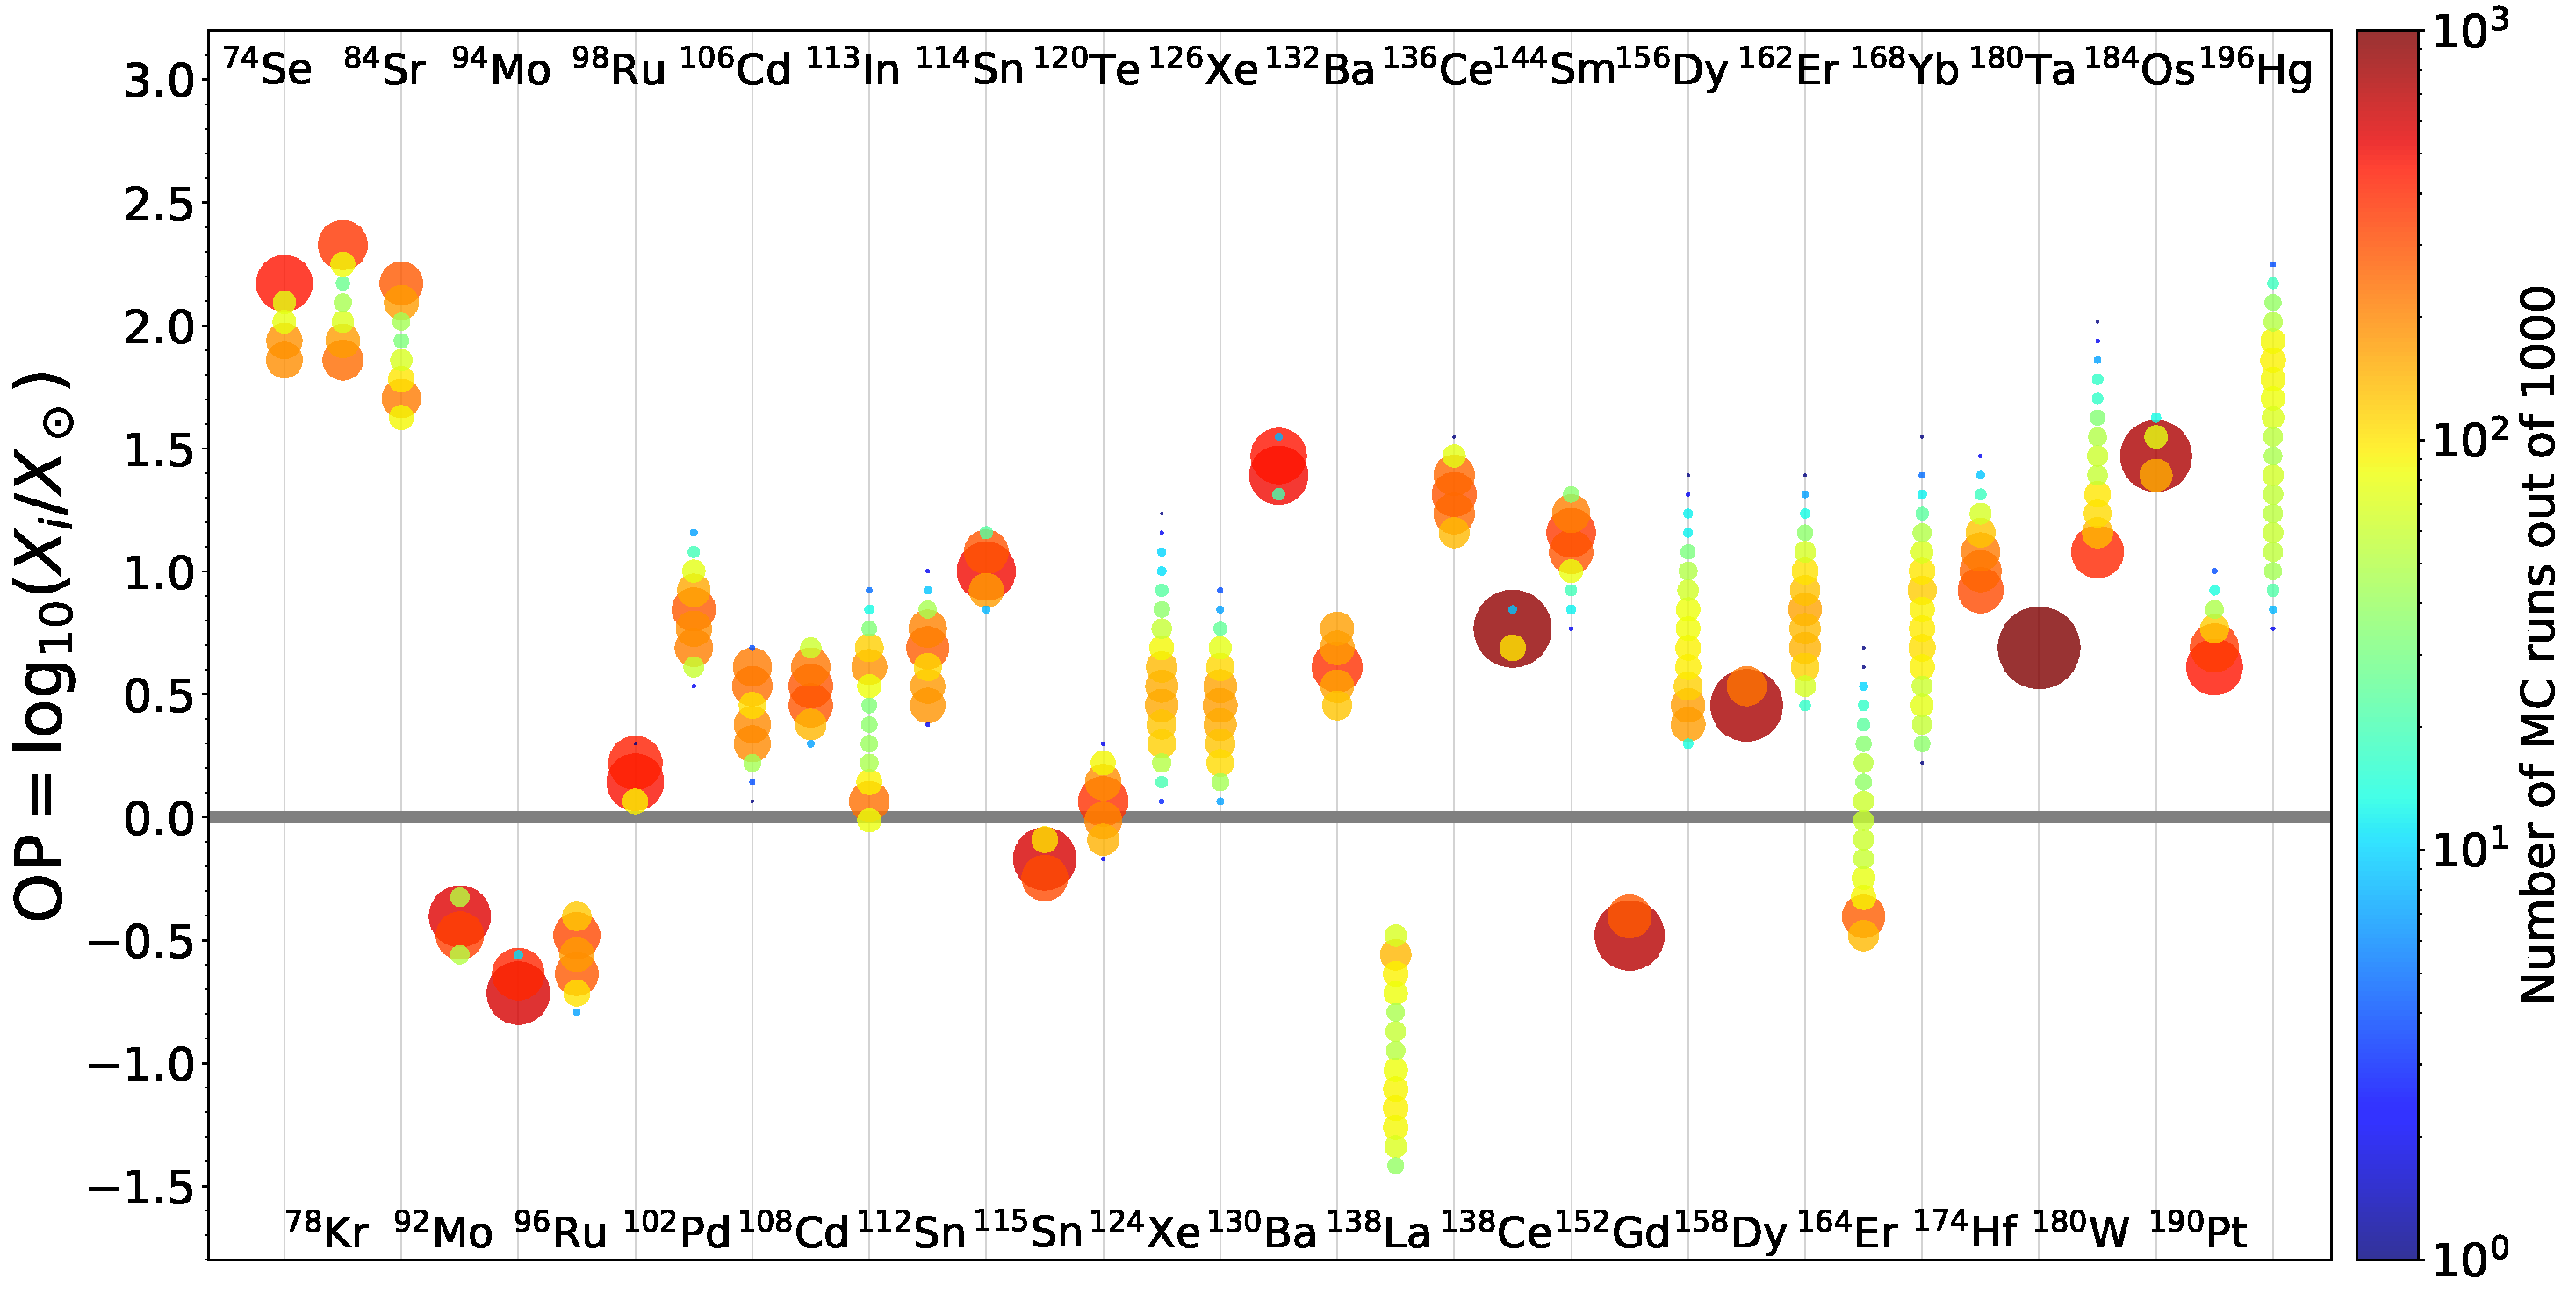
\includegraphics[width=\textwidth]{chapters/2/figures/nuclearimpact_MLT.pdf}
\caption{Histogram showing the spread due to varying $(\gamma,p)$, $(\gamma,n)$, $(\gamma,\alpha)$ and corresponding capture rates for unstable p-heavy isotopes from Se-Po for the MLT mixing scenario. Colour and size correspond to the logarthimic binning of Monte Carlo runs. The thick grey line at $\mathrm{OP} = 0$ corresponds to the solar measurement. The average spread in production is $0.56~\mathrm{dex}$.
\label{fig:nuclearimpact_MLT}}
\end{figure}

\begin{figure}[!htbp]
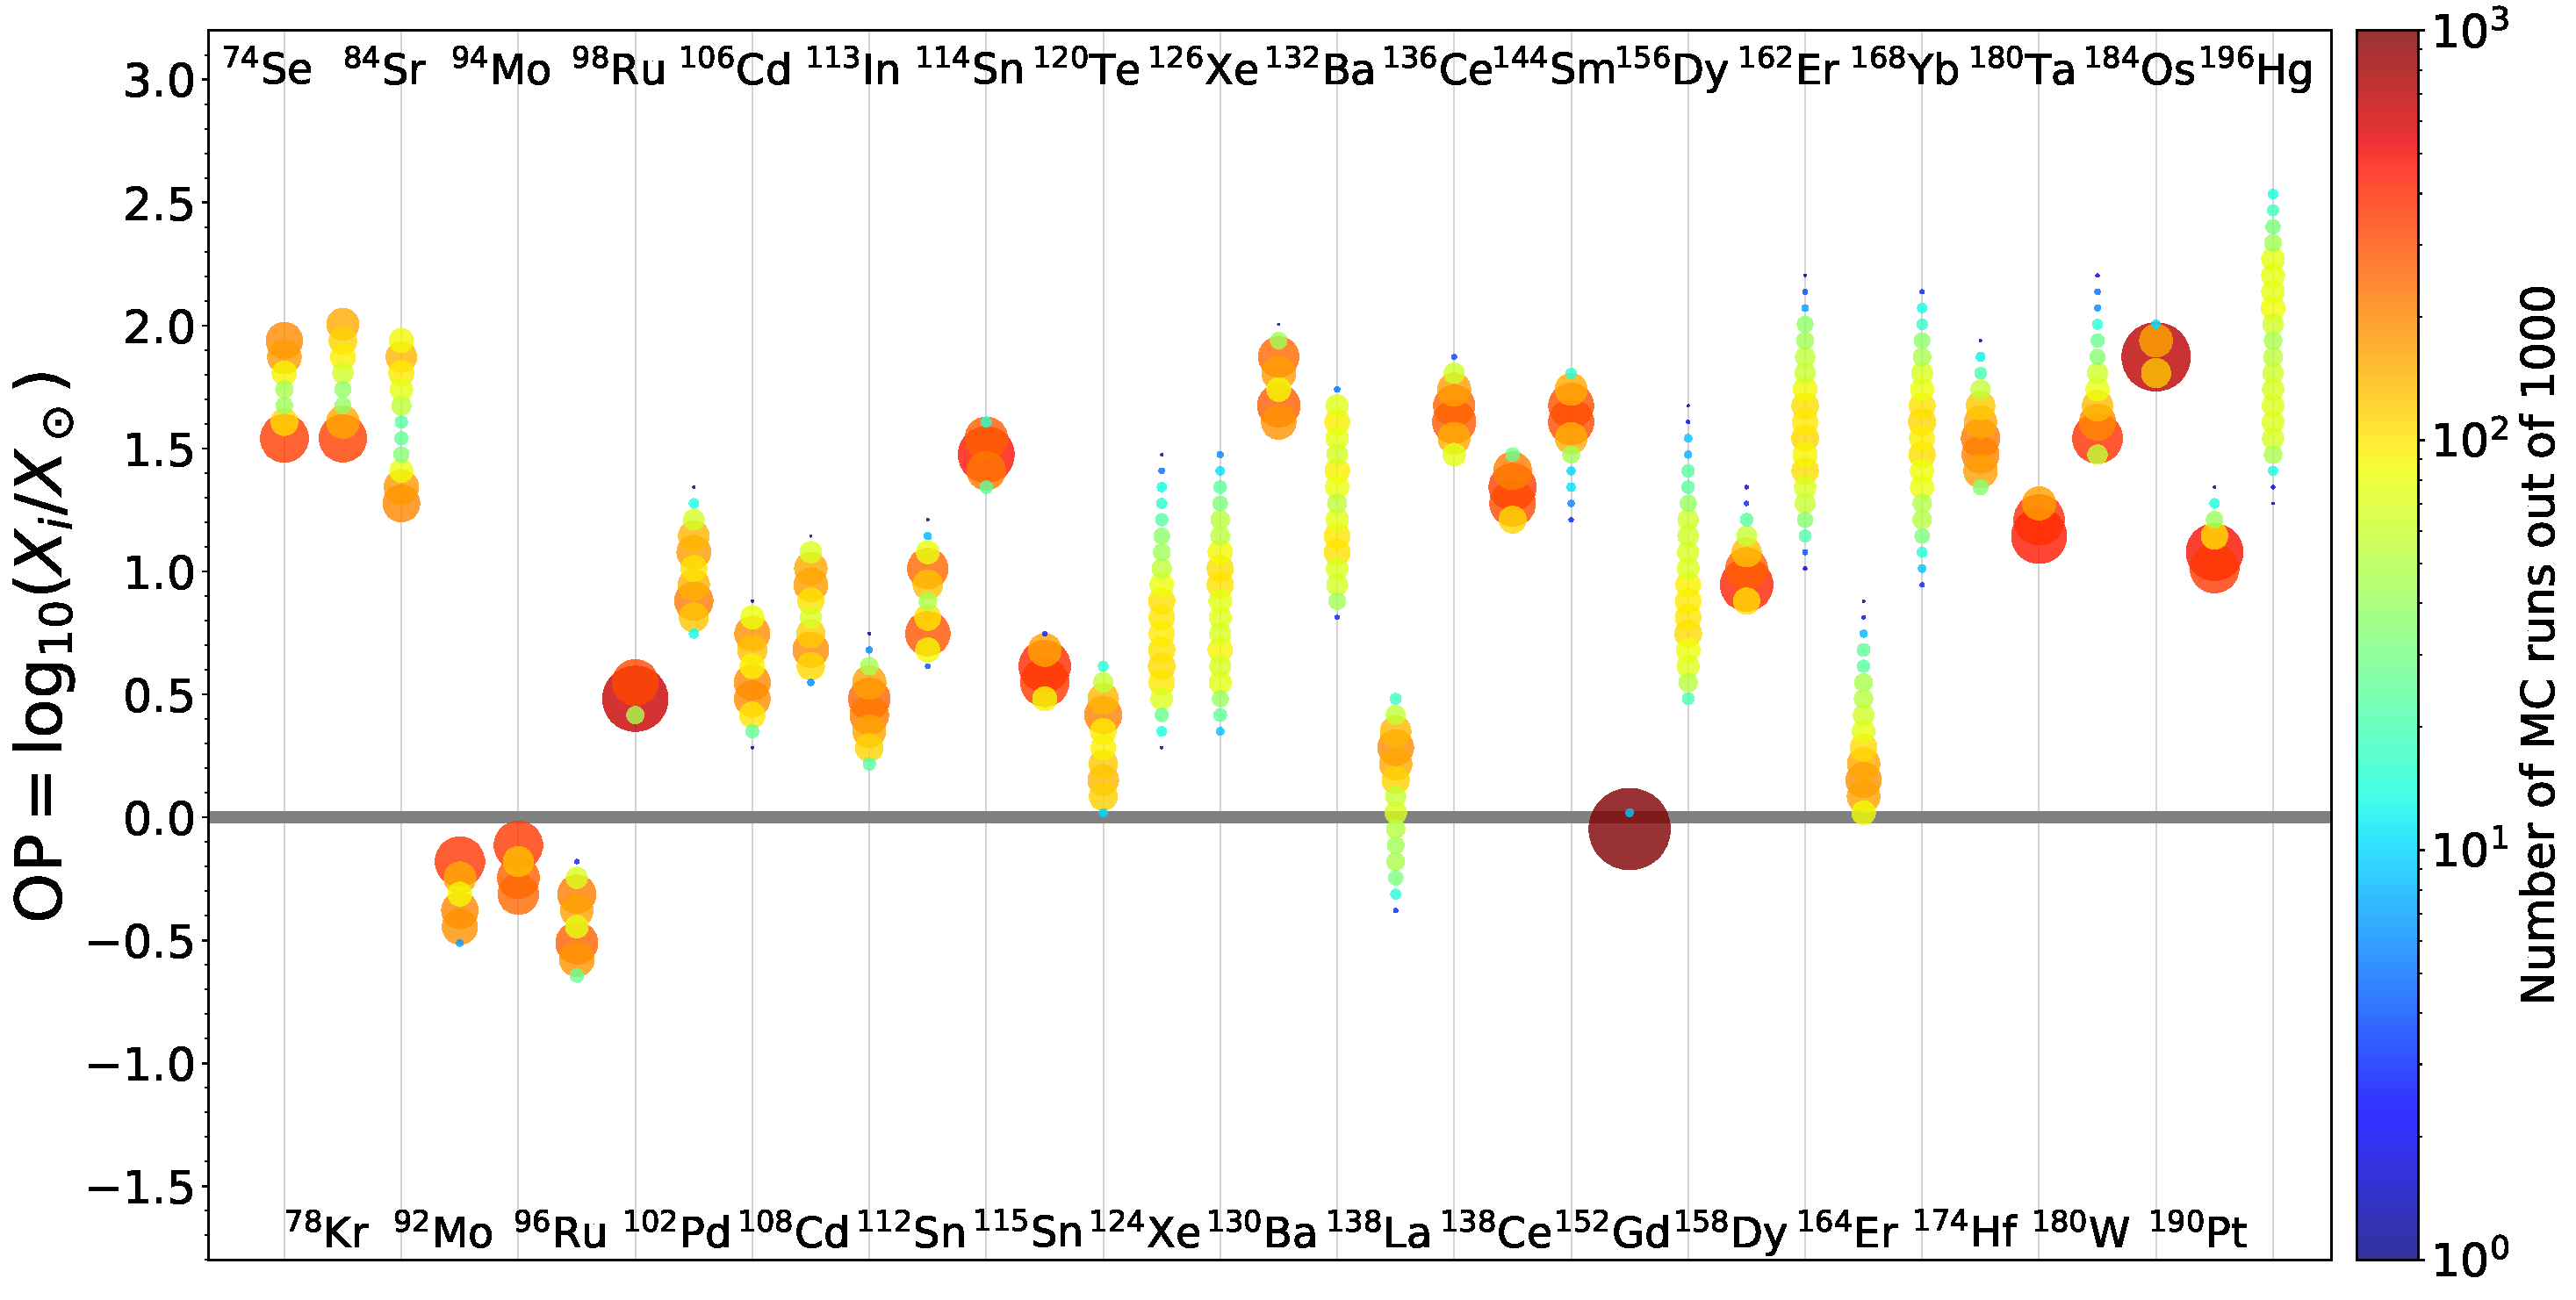
\includegraphics[width=\textwidth]{chapters/2/figures/nuclearimpact_3D.pdf}
\caption{Histogram showing the spread due to varying $(\gamma,p)$, $(\gamma,n)$, $(\gamma,\alpha)$ and corresponding capture rates for unstable p-heavy isotopes from Se-Po for the 3D-inspired mixing scenario. The thick grey line at $\mathrm{OP} = 0$ corresponds to the solar measurement. The average spread in production is $0.59~\mathrm{dex}$.
\label{fig:nuclearimpact_3D}}
\end{figure}

\begin{figure}[!htbp]
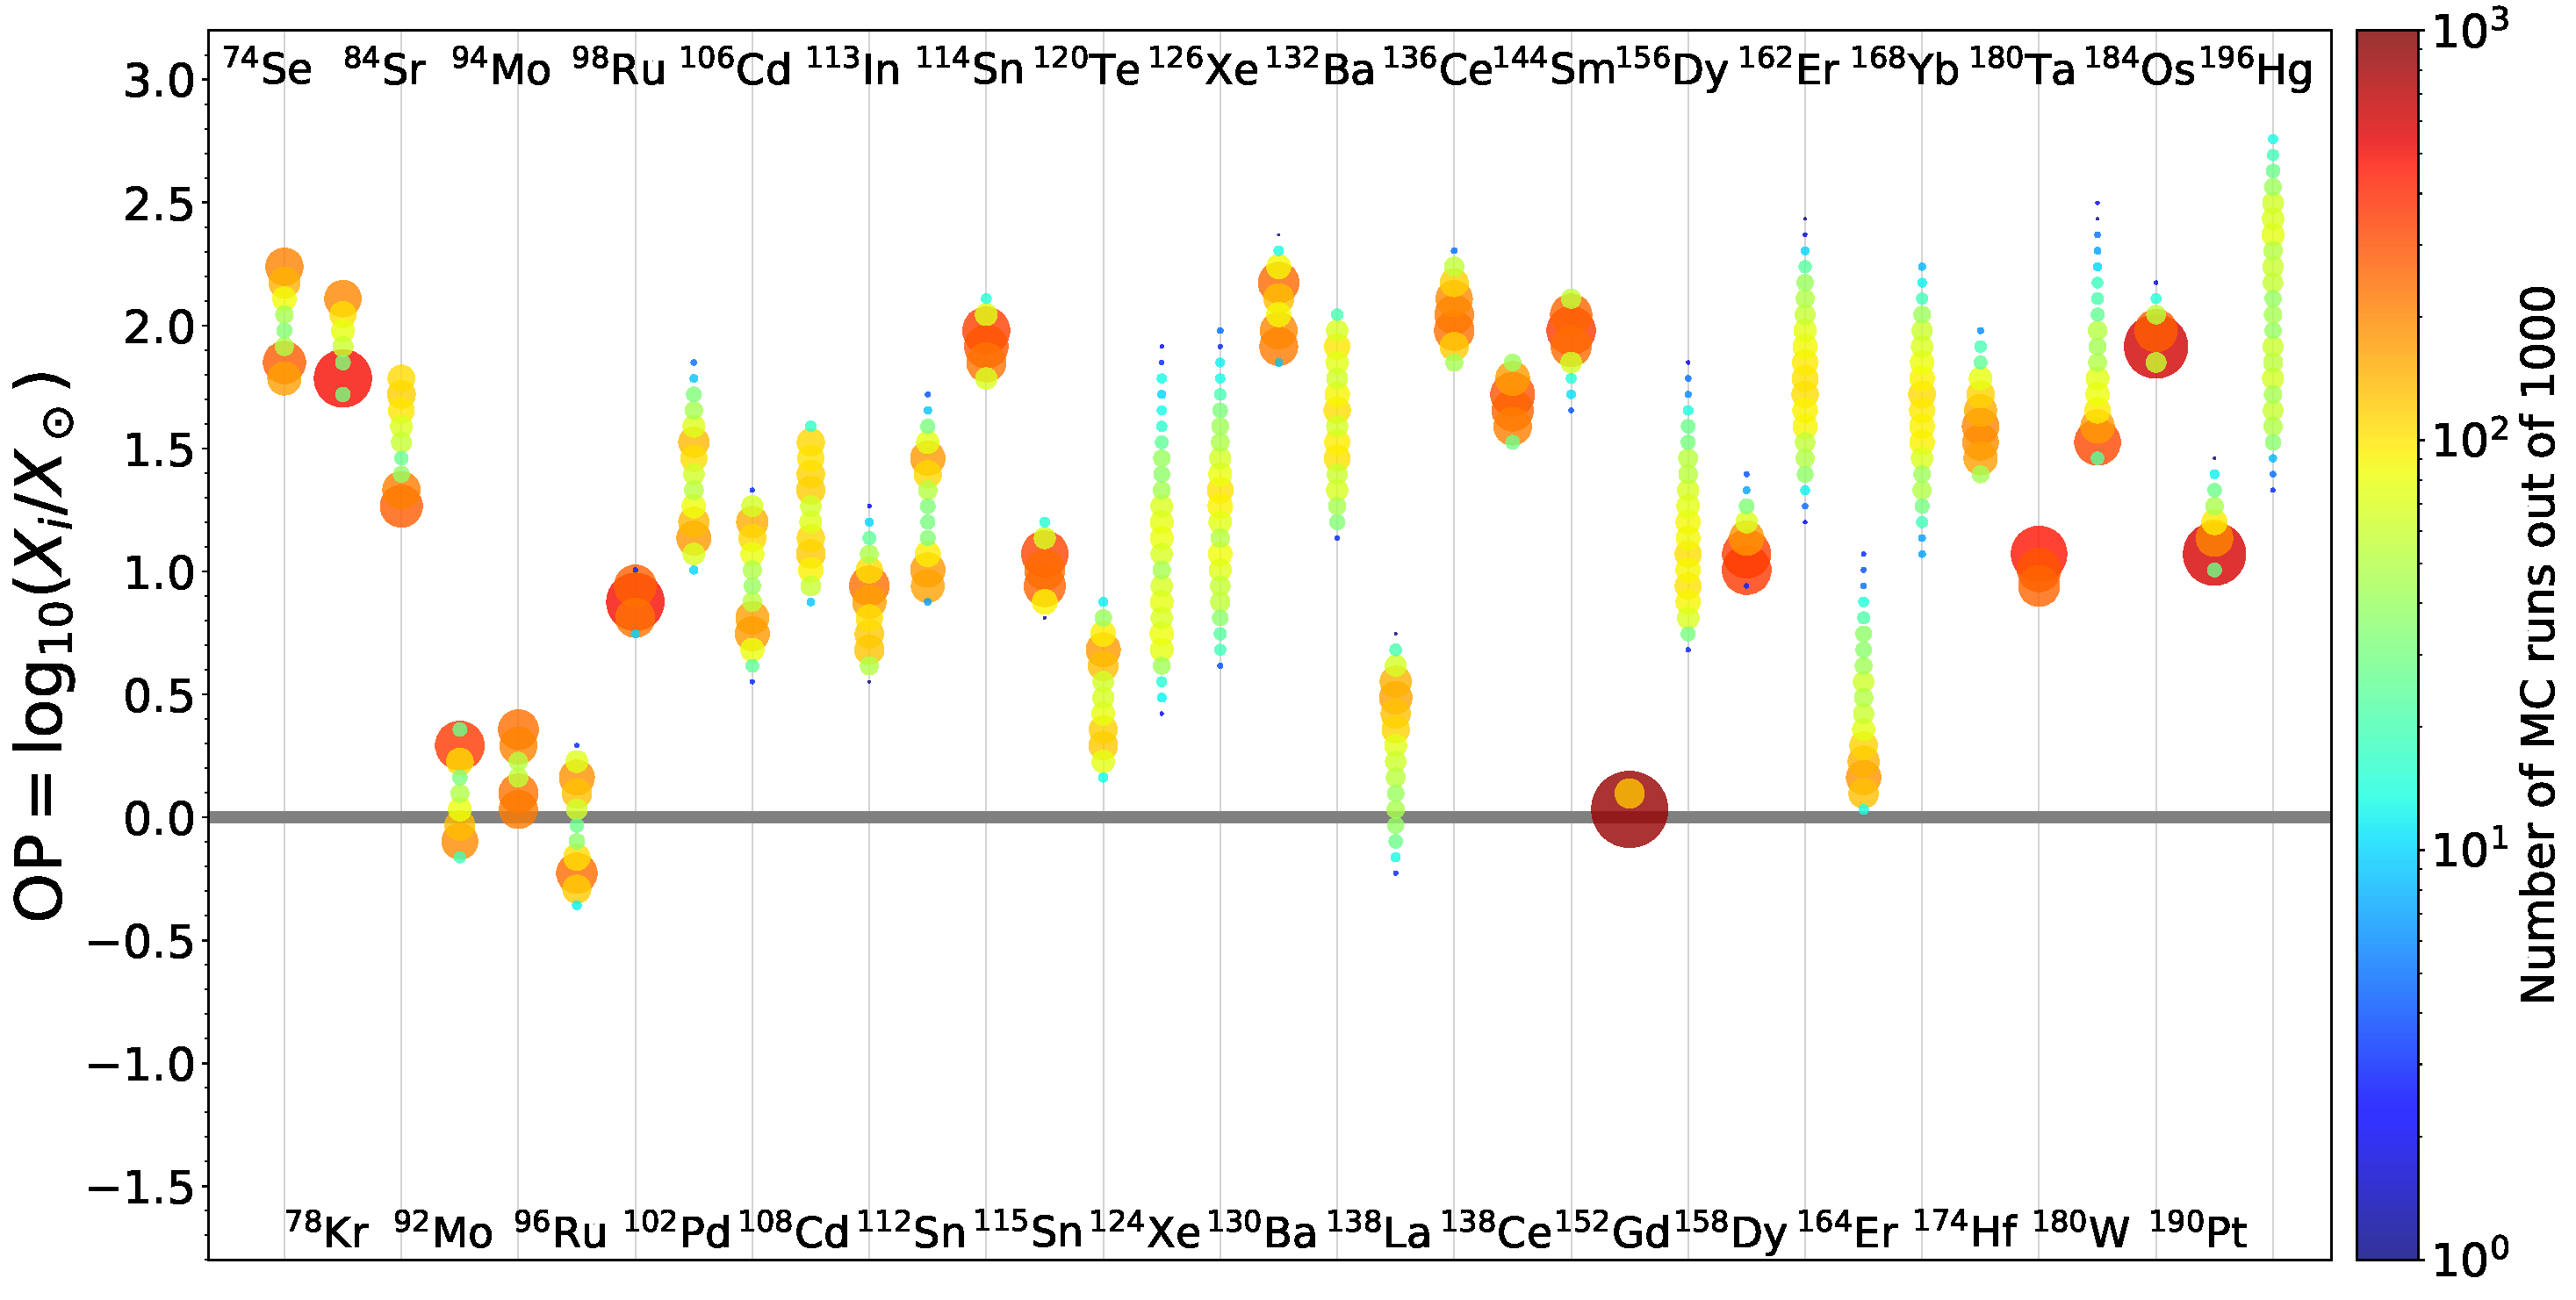
\includegraphics[width=\textwidth]{chapters/2/figures/nuclearimpact_3x3D.pdf}
\caption{Histogram showing the spread due to varying $(\gamma,p)$, $(\gamma,n)$, $(\gamma,\alpha)$ and corresponding capture rates for unstable p-heavy isotopes from Se-Po for the $3\times$3D-inspired mixing scenario. The thick grey line at $\mathrm{OP} = 0$ corresponds to the solar measurement. The average spread in production is $0.69~\mathrm{dex}$.
\label{fig:nuclearimpact_3x3D}}
\end{figure}

\begin{figure}[!htbp]
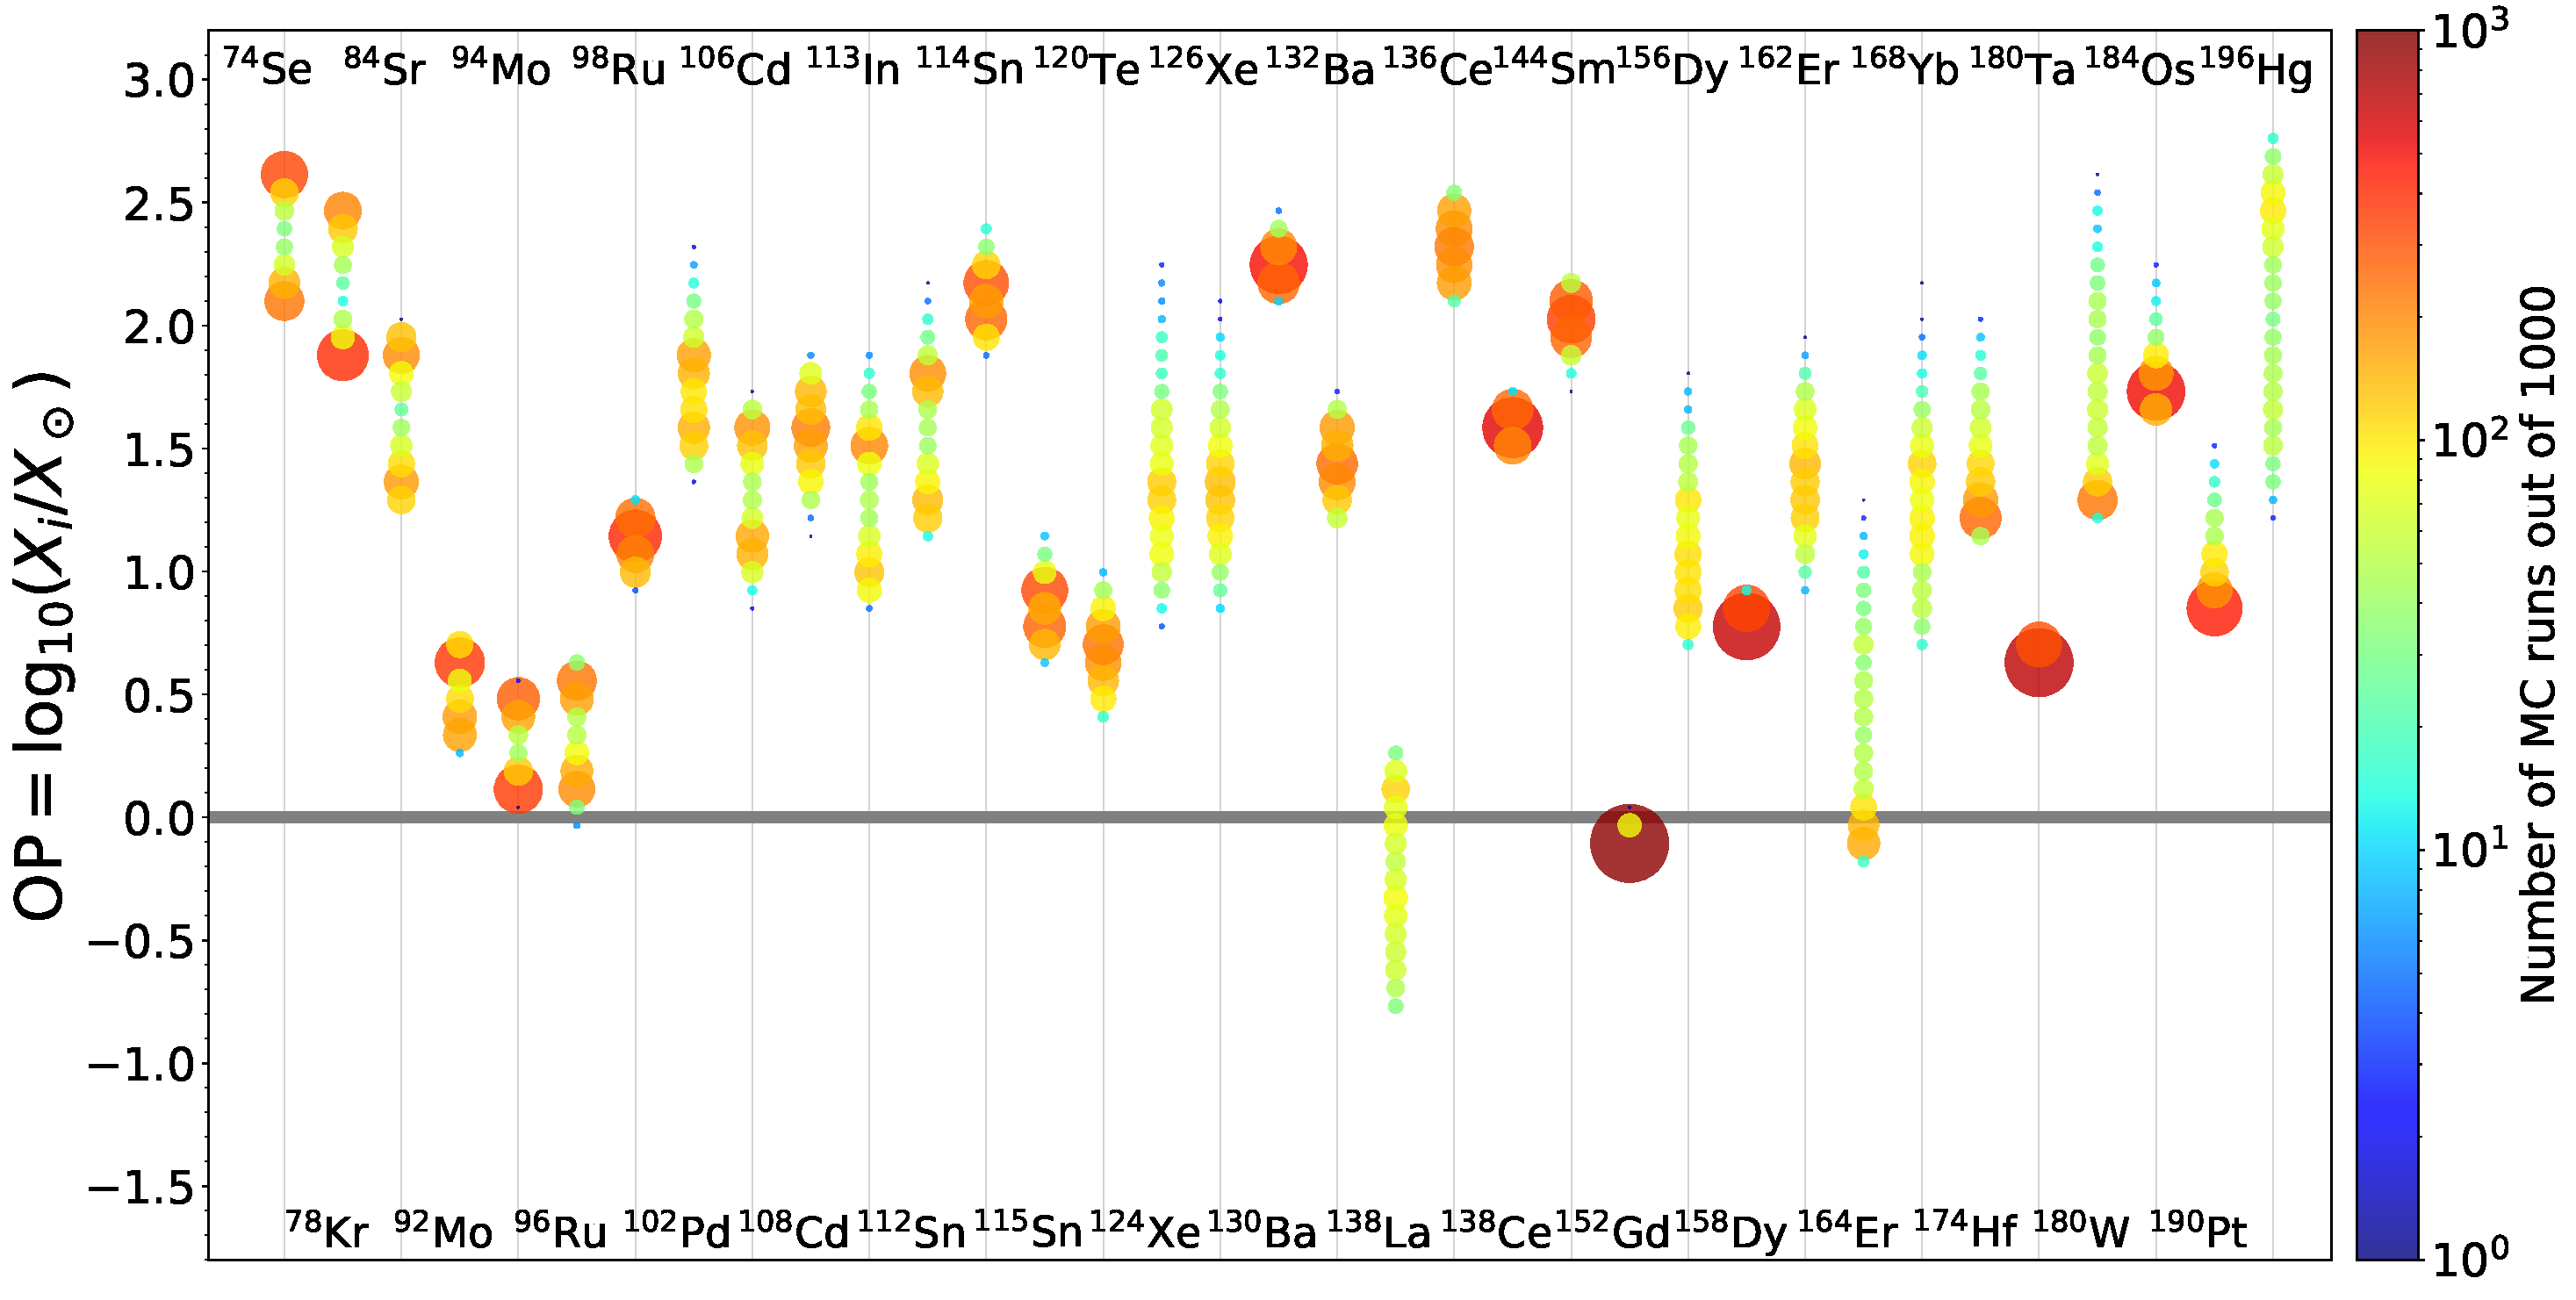
\includegraphics[width=\textwidth]{chapters/2/figures/nuclearimpact_10x3D.pdf}
\caption{Histogram showing the spread due to varying $(\gamma,p)$, $(\gamma,n)$, $(\gamma,\alpha)$ and corresponding capture rates for unstable p-heavy isotopes from Se-Po for the $10\times$3D-inspired mixing scenario. The thick grey line at $\mathrm{OP} = 0$ corresponds to the solar measurement. The average spread in production is $0.76~\mathrm{dex}$.
\label{fig:nuclearimpact_10x3D}}
\end{figure}

\begin{figure}[!htbp]
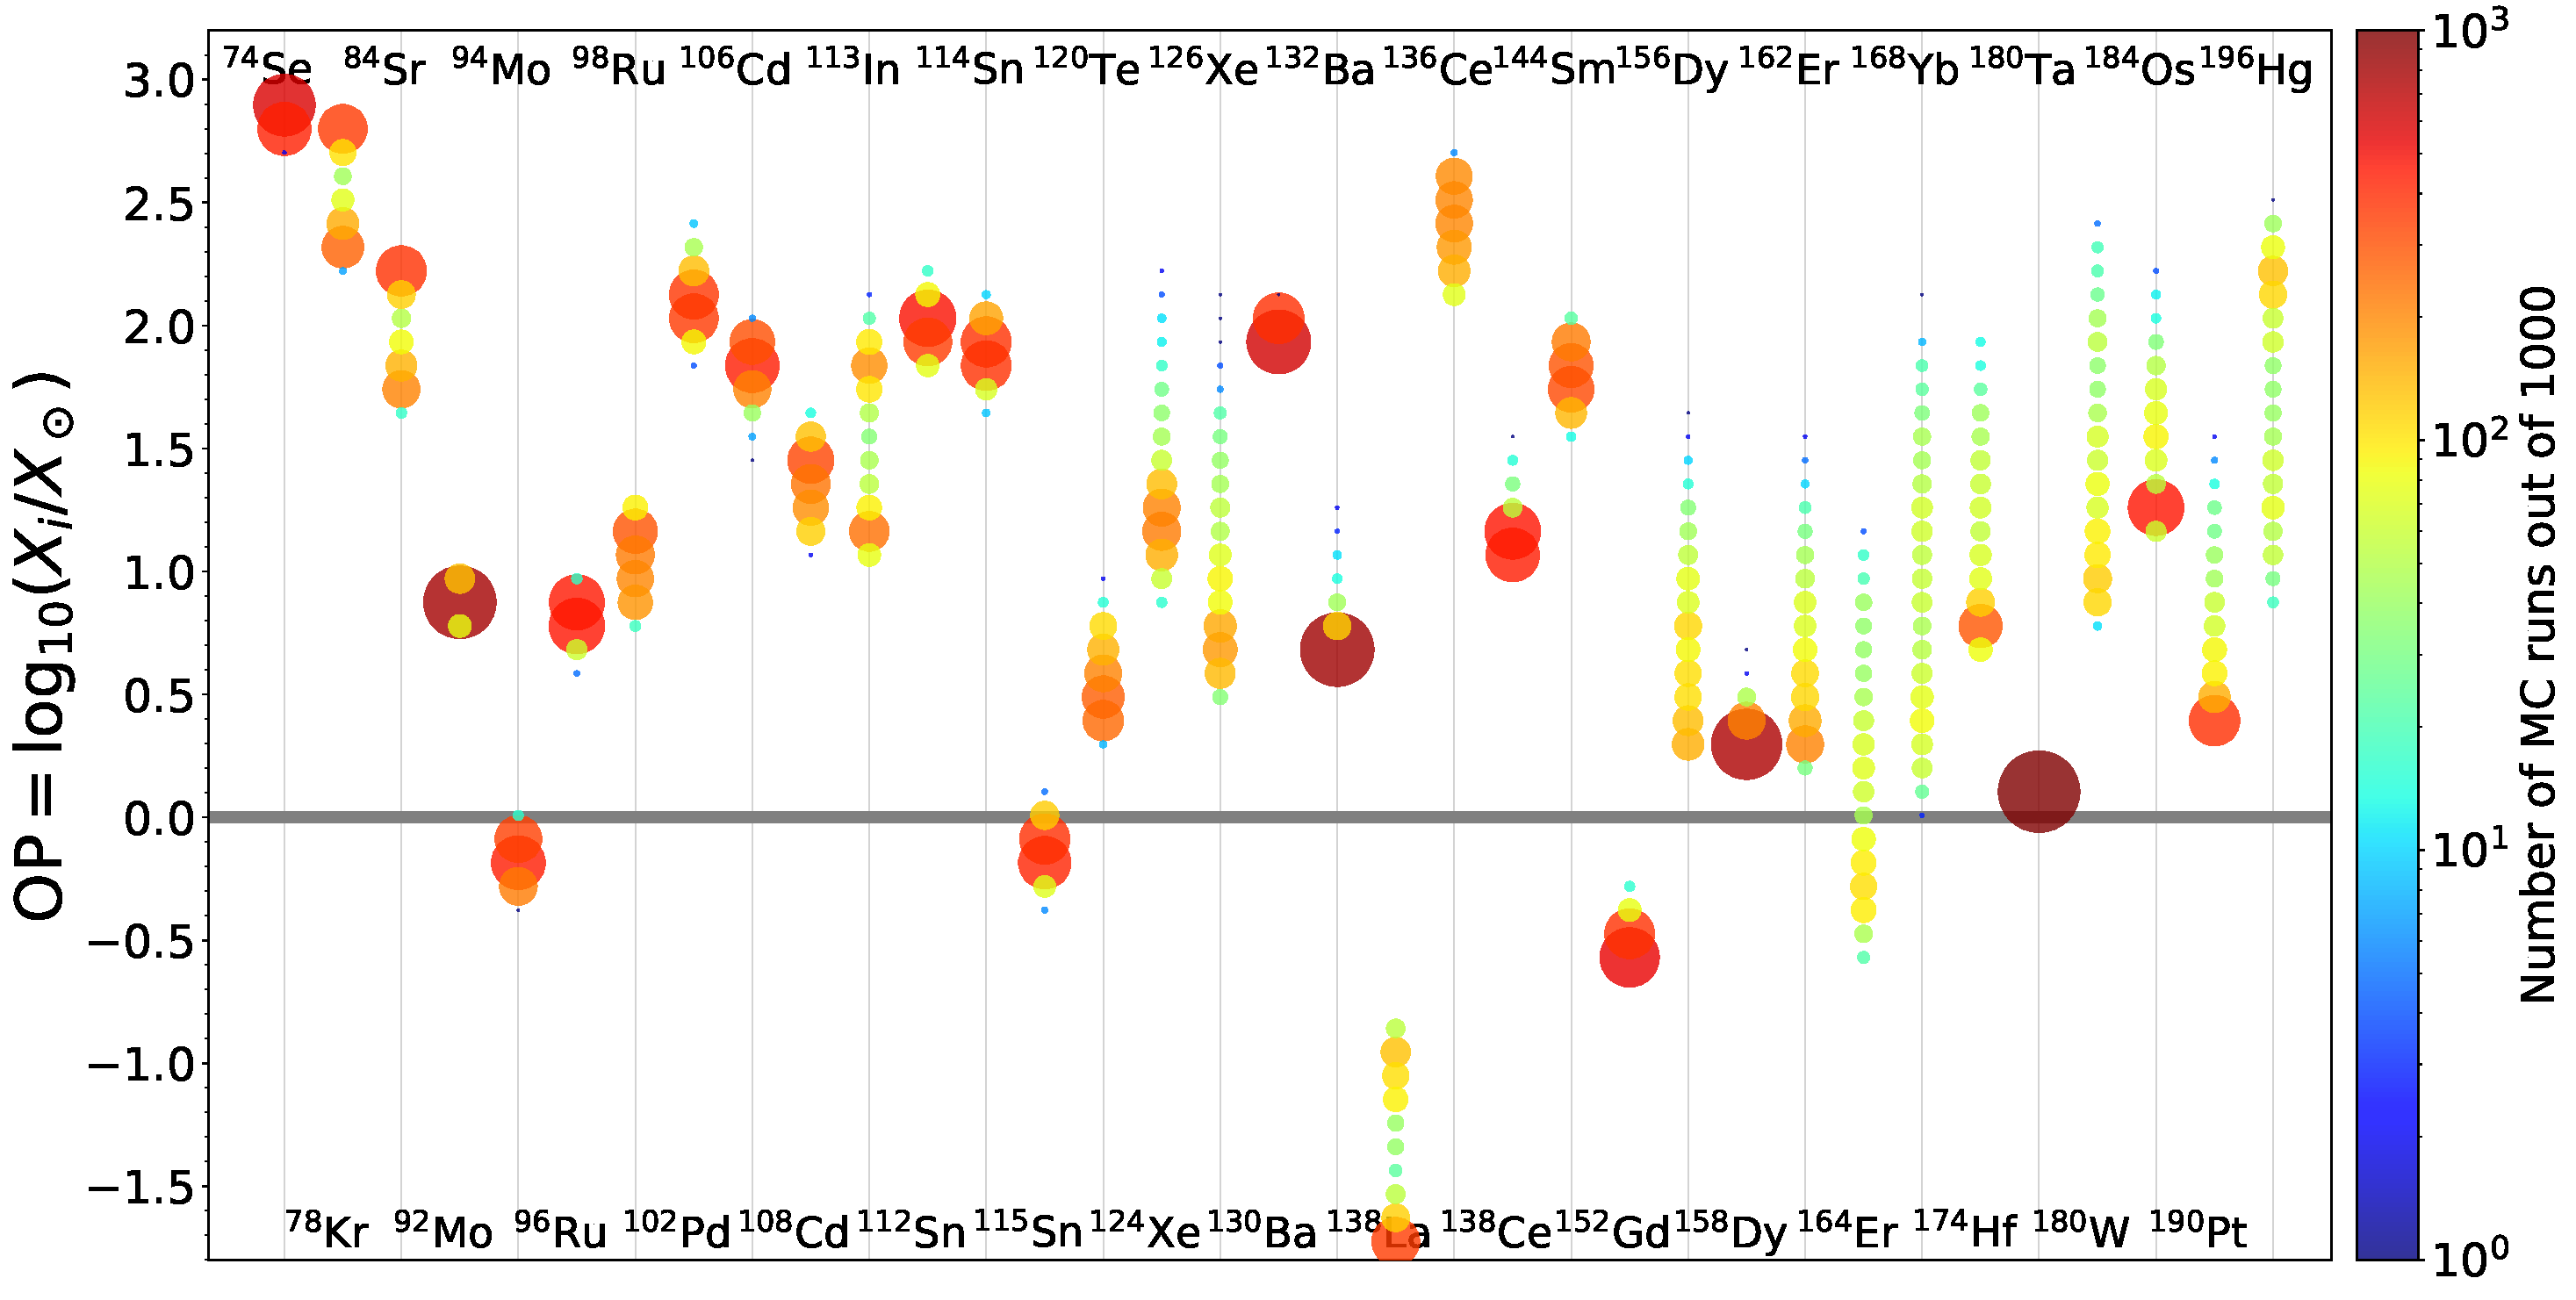
\includegraphics[width=\textwidth]{chapters/2/figures/nuclearimpact_50x3D.pdf}
\caption{Histogram showing the spread due to varying $(\gamma,p)$, $(\gamma,n)$, $(\gamma,\alpha)$ and corresponding capture rates for unstable p-heavy isotopes from Se-Po for the $50\times$3D-inspired mixing scenario. The thick grey line at $\mathrm{OP} = 0$ corresponds to the solar measurement. The average spread in production is $0.79~\mathrm{dex}$.
\label{fig:nuclearimpact_50x3D}}
\end{figure}

The MLT scenario shows that most of the p-nuclei are impacted by varying the photo-disintegration rates although the spread is very different depending on the isotope, and the $1\times$ convective downturn scenario already shows a significant change in how varying the nuclear physics impacts the same species.
As mixing speeds increase, the spread increases for most isotopes.
The average spread in production for the MLT and $1\times$, $3\times$, $10\times$, $50\times$ boosted convective downturn scenarios are $0.56 ~\mathrm{dex}$, $0.59 ~\mathrm{dex}$, $0.69 ~\mathrm{dex}$, $0.76 ~\mathrm{dex}$, and $0.79 ~\mathrm{dex}$ respectively.
This demonstrates how the mixing details matter when considering the nuclear physics impact as this is a convective-reactive environment.

The average spread in production increases with mixing speed because the material is able to reach hotter temperatures and the possible nucleosynthetic pathways increase.
Species like $^{180}\mathrm{W}$ and $^{196}\mathrm{Hg}$ have a spread that increases with mixing speed.
This growth is not linear for all species though as those like $^{74}\mathrm{Se}$ and $^{92}\mathrm{Mo}$ grow with mixing speed except for the fastest $50\times$ scenario where the spread decreases.
There are also impacts on whether the final mass fraction distribution of a species is double peaked and the magnitude of those peaks.
$^{96}\mathrm{Ru}$, $^{113}\mathrm{In}$, $^{130}\mathrm{Ba}$, $^{138}\mathrm{La}$ are isotopes where the presence of a double peak in the final mass fraction is dependent on the mixing scenario. 
$^{74}\mathrm{Se}$, $^{78}\mathrm{Kr}$, and $^{84}\mathrm{Sr}$ both have a double peak across the mixing scenarios, but the magnitude of those peaks and whether the higher $\mathrm{OP}$ or lower $\mathrm{OP}$ peak are favoured is dependent on mixing scenario.
This has an implication for using distributions

Considering the reaction rates correlations, whether a particular rate is correlated with the production of a species is completely dependent on the mixing scenario along with the strength of the correlation.
Table \ref{tab:unique_rates} lists those that are unique to a single scenario.

\begin{table*}
\caption{Reactions correlated with the production/destruction of an isotope unique to an individual mixing scenario.
\label{tab:unique_rates}}
\begin{tabular}{l|l}
    \toprule
    \multicolumn{1}{c}{\textbf{Isotope}} & \multicolumn{1}{c}{\textbf{Unique Correlated Reaction Rates}} \\
    \toprule
    \multicolumn{2}{c}{\textbf{MLT Mixing Case}} \\
    \midrule
    $^{138}\mathrm{Ce}$ & $^{139}\mathrm{Pr}(\gamma,p)$ \\
    $^{168}\mathrm{Yb}$ & $^{176}\mathrm{W}(\gamma,\alpha)$ \\
    $^{174}\mathrm{Hf}$ & $^{178}\mathrm{W}(\gamma,n)$ \\
    $^{184}\mathrm{Os}$ & $^{186}\mathrm{Pt}(\gamma,n)$~~$^{188}\mathrm{Pt}(\gamma,n)$ \\
    \midrule
    \multicolumn{2}{c}{\textbf{3D-inspired Mixing Case}} \\
    \midrule
    $^{113}\mathrm{In}$ & $^{114}\mathrm{In}(\gamma,n)$ \\
    $^{152}\mathrm{Gd}$ & $^{150}\mathrm{Gd}(\gamma,\alpha)$~~$^{196}\mathrm{Pb}(\gamma,n)$ \\
    $^{180}\mathrm{Ta}$ & $^{179}\mathrm{Ta}(\gamma,\alpha)$ \\
    \midrule
    \multicolumn{2}{c}{$\mathbf{3\times}$\textbf{3D-inspired Mixing Case}} \\
    \midrule
    $^{180}\mathrm{W}$ & $^{181}\mathrm{Os}(\gamma,n)$ \\
    \midrule
    \multicolumn{2}{c}{$\mathbf{10\times}$\textbf{3D-inspired Mixing Case}} \\
    \midrule
    $^{84}\mathrm{Sr}$ & $^{84}\mathrm{Rb}(\gamma,n)$ \\
    $^{120}\mathrm{Te}$ & $^{119}\mathrm{Te}(\gamma,n)$ \\
    $^{126}\mathrm{Xe}$ & $^{122}\mathrm{Xe}(\gamma,n)$ \\
    $^{130}\mathrm{Ba}$ & $^{126}\mathrm{Ba}(\gamma,p)$~~$^{128}\mathrm{Ba}(\gamma,\alpha)$~~$^{128}\mathrm{Ba}(\gamma,p)$ \\
    $^{132}\mathrm{Ba}$ & $^{128}\mathrm{Ba}(\gamma,\alpha)$ \\
    $^{168}\mathrm{Yb}$ & $^{169}\mathrm{Hf}(\gamma,n)$ \\
    $^{174}\mathrm{Hf}$ & $^{176}\mathrm{W}(\gamma,\alpha)$ \\
    $^{184}\mathrm{Os}$ & $^{185}\mathrm{Pt}(\gamma,\alpha)$ \\
    \midrule
    \multicolumn{2}{c}{$\mathbf{50\times}$\textbf{3D-inspired Mixing Case}} \\
    \midrule
    $^{92}\mathrm{Mo}$ & $^{100}\mathrm{Pd}(\gamma,\alpha)$~~$^{100}\mathrm{Pd}(\gamma,p)$~~$^{110}\mathrm{Sn}(\gamma,n)$~~$^{110}\mathrm{Sn}(\gamma,p)$ \\
    $^{96}\mathrm{Ru}$ & $^{97}\mathrm{Ru}(\gamma,\alpha)$~~$^{110}\mathrm{Sn}(\gamma,\alpha)$~~$^{110}\mathrm{Sn}(\gamma,n)$~~$^{110}\mathrm{Sn}(\gamma,p)$ \\
    $^{102}\mathrm{Pd}$ & $^{104}\mathrm{Cd}(\gamma,\alpha)$~~$^{104}\mathrm{Cd}(\gamma,p)$ \\
    $^{106}\mathrm{Cd}$ & $^{104}\mathrm{Cd}(\gamma,p)$~~$^{110}\mathrm{Sn}(\gamma,p)$ \\
    $^{108}\mathrm{Cd}$ & $^{110}\mathrm{Sn}(\gamma,\alpha)$ \\
    $^{112}\mathrm{Sn}$ & $^{110}\mathrm{Sn}(\gamma,p)$ \\
    $^{115}\mathrm{Sn}$ & $^{122}\mathrm{Xe}(\gamma,n)$ \\
    $^{120}\mathrm{Te}$ & $^{120}\mathrm{Xe}(\gamma,\alpha)$ \\
    $^{126}\mathrm{Xe}$ & $^{127}\mathrm{Ba}(\gamma,n)$ \\
    $^{130}\mathrm{Ba}$ & $^{132}\mathrm{Ce}(\gamma,\alpha)$~~$^{132}\mathrm{Ce}(\gamma,n)$~~$^{132}\mathrm{Ce}(\gamma,p)$\\
    &$^{134}\mathrm{Ce}(\gamma,\alpha)$~~$^{134}\mathrm{Ce}(\gamma,n)$ \\
    $^{132}\mathrm{Ba}$ & $^{132}\mathrm{Ce}(\gamma,\alpha)$~~$^{132}\mathrm{Ce}(\gamma,n)$~~$^{132}\mathrm{Ce}(\gamma,p)$\\
    & $^{133}\mathrm{Ce}(\gamma,n)$~~$^{134}\mathrm{Ce}(\gamma,\alpha)$ \\
    $^{138}\mathrm{Ce}$ & $^{139}\mathrm{Nd}(\gamma,n)$ \\
    $^{156}\mathrm{Dy}$ & $^{156}\mathrm{Er}(\gamma,\alpha)$~~$^{158}\mathrm{Er}(\gamma,\alpha)$~~$^{158}\mathrm{Er}(\gamma,n)$ \\
    $^{162}\mathrm{Er}$ & $^{168}\mathrm{Hf}(\gamma,n)$~~$^{162}\mathrm{Yb}(\gamma,\alpha)$~~$^{164}\mathrm{Yb}(\gamma,\alpha)$ \\
    $^{184}\mathrm{Os}$ & $^{184}\mathrm{Pt}(\gamma,n)$ \\
    \toprule
\end{tabular}
\end{table*}

If one wants to propose experiments based on the astrophysical site of an O-C merger, the nuances of the mixing details should be taken into account.
For instance, the $50\times$3D-inspired mixing scenario has the largest number of unique reactions as the material is able to advect to the hottest temperatures before reacting, and therefore has a more complex nucleosynthetic pathway.
Whether a reaction rate is identified as important and the level of that importance both depend on the whether a convective downturn is present and the speed of mixing.

This is not to say that there aren't shared reactions across the mixing scenarios, as all those that are listed in Table \ref{tab:shared_rates} are shared across mixing scenario.
However, just because these rates are shared does not mean that they are all strongly correlated with the production of the p-nuclei, nor does it mean that they are all impactful in every case.
For example, all scenarios have a correlation of $X(^{156}\mathrm{Dy})$ with $^{160}\mathrm{Er}(\gamma,\alpha)$, but in the $50\times$3D-inspired the correlation is much weaker.
This underscores the difficulty in using 1-D astrophysical sites to identify important reactions for nuclear physics experiments.

There is a way that nuclear experiments could discriminate mixing scenarios as there are reactions unique to the MLT mixing scenario as listed in Table \ref{tab:unique_rates} and there are two reaction rates that are correlated in all convective downturns scenarios but not in the MLT case which are  $X(^{115}\mathrm{Sn})$ with $^{110}\mathrm{Sn}(\gamma,\alpha)$ and $X(^{138}\mathrm{Ce})$ with $^{138}\mathrm{Nd}(\gamma,p)$. 

\begin{table*}
\caption{Reactions correlated with the production/destruction of an isotope shared across all mixing scenarios.
\label{tab:shared_rates}}
\begin{tabular}{l|l}
    \toprule
    \textbf{Isotope} & \textbf{Shared Correlated Reaction Rates} \\ 
    \toprule
    $^{74}\mathrm{Se}$ & $^{75}\mathrm{Se}(\gamma,n)$ \\
    $^{78}\mathrm{Kr}$ & $^{79}\mathrm{Kr}(\gamma,n)$ \\
    $^{84}\mathrm{Sr}$ & $^{85}\mathrm{Sr}(\gamma,n)$ \\
    $^{92}\mathrm{Mo}$ & $^{93}\mathrm{Mo}(\gamma,n)$ \\
    $^{94}\mathrm{Mo}$ & $^{93}\mathrm{Mo}(\gamma,n)$ \\
    $^{96}\mathrm{Ru}$ & $^{97}\mathrm{Ru}(\gamma,n)$ \\
    $^{98}\mathrm{Ru}$ & $^{100}\mathrm{Pd}(\gamma,\alpha)$~~$^{100}\mathrm{Pd}(\gamma,p)$ \\
    $^{102}\mathrm{Pd}$ & $^{100}\mathrm{Pd}(\gamma,\alpha)$~~$^{100}\mathrm{Pd}(\gamma,p)$~~$^{103}\mathrm{Pd}(\gamma,n)$ \\
    $^{106}\mathrm{Cd}$ & $^{107}\mathrm{Cd}(\gamma,n)$~~$^{110}\mathrm{Sn}(\gamma,\alpha)$ \\
    $^{108}\mathrm{Cd}$ & $^{107}\mathrm{Cd}(\gamma,n)$ \\
    $^{113}\mathrm{In}$ & $^{113}\mathrm{Sn}(\gamma,n)$ \\
    $^{112}\mathrm{Sn}$ & $^{113}\mathrm{Sn}(\gamma,n)$ \\
    $^{114}\mathrm{Sn}$ & $^{110}\mathrm{Sn}(\gamma,\alpha)$~~$^{113}\mathrm{Sn}(\gamma,n)$~~$^{122}\mathrm{Xe}(\gamma,\alpha)$ \\
    $^{115}\mathrm{Sn}$ & $^{113}\mathrm{Sn}(\gamma,n)$ \\
    $^{120}\mathrm{Te}$ & $^{122}\mathrm{Xe}(\gamma,\alpha)$~~$^{122}\mathrm{Xe}(\gamma,p)$ \\
    $^{124}\mathrm{Xe}$ & $^{122}\mathrm{Xe}(\gamma,\alpha)$~~$^{122}\mathrm{Xe}(\gamma,p)$ \\
    $^{138}\mathrm{La}$ & $^{137}\mathrm{La}(\gamma,n)$ \\
    $^{136}\mathrm{Ce}$ & $^{138}\mathrm{Nd}(\gamma,n)$~~$^{138}\mathrm{Nd}(\gamma,p)$~~$^{140}\mathrm{Nd}(\gamma,\alpha)$ \\
    $^{144}\mathrm{Sm}$ & $^{196}\mathrm{Pb}(\gamma,n)$~~$^{142}\mathrm{Sm}(\gamma,n)$~~$^{142}\mathrm{Sm}(\gamma,p)$~~$^{143}\mathrm{Sm}(\gamma,n)$ \\
    $^{152}\mathrm{Gd}$ & $^{152}\mathrm{Dy}(\gamma,\alpha)$ \\
    $^{156}\mathrm{Dy}$ & $^{160}\mathrm{Er}(\gamma,\alpha)$ \\
    $^{164}\mathrm{Er}$ & $^{164}\mathrm{Yb}(\gamma,\alpha)$~~$^{164}\mathrm{Yb}(\gamma,n)$ \\
    $^{174}\mathrm{Hf}$ & $^{174}\mathrm{W}(\gamma,\alpha)$ \\
    $^{180}\mathrm{Ta}$ & $^{179}\mathrm{Ta}(\gamma,n)$ \\
    $^{180}\mathrm{W}$ & $^{180}\mathrm{Os}(\gamma,\alpha)$~~$^{180}\mathrm{Os}(\gamma,n)$~~$^{196}\mathrm{Pb}(\gamma,n)$ \\
    $^{184}\mathrm{Os}$ & $^{196}\mathrm{Pb}(\gamma,n)$~~$^{184}\mathrm{Pt}(\gamma,\alpha)$ \\
    $^{190}\mathrm{Pt}$ & $^{190}\mathrm{Hg}(\gamma,\alpha)$~~$^{190}\mathrm{Hg}(\gamma,n)$~~$^{196}\mathrm{Pb}(\gamma,n)$ \\
    $^{196}\mathrm{Hg}$ & $^{196}\mathrm{Pb}(\gamma,n)$~~$^{202}\mathrm{Pb}(\gamma,n)$ \\
    \toprule
    \end{tabular}
\end{table*}

\begin{table*}
\caption{Correlations and $\zeta$ slopes between mass fraction and reaction rates for the MLT mixing scenario.
\label{tab:mlt_corr}}
\scriptsize
    \begin{tabular}{llcc|llcc}
    \toprule
    \textbf{Isotope} & \textbf{Reaction} & $\mathbf{r_\mathrm{\mathbf{P}}}$ & $\mathbf{\zeta}$ & \textbf{Isotope} & \textbf{Reaction} & $\mathbf{r_\mathrm{\mathbf{P}}}$ & $\mathbf{\zeta}$ \\
    \toprule
    $^{74}\mathrm{Se}$ & $^{75}\mathrm{Se}(\gamma,n)$ & $-0.93$ & $-0.18$ & $^{144}\mathrm{Sm}$ & $^{142}\mathrm{Sm}(\gamma,n)$ & $-0.19$ & $-0.02$ \\ 
    $^{78}\mathrm{Kr}$ & $^{79}\mathrm{Kr}(\gamma,n)$ & $-0.88$ & $-0.28$ & $ $ & $^{142}\mathrm{Sm}(\gamma,p)$ & $-0.17$ & $-0.02$ \\ 
    $^{84}\mathrm{Sr}$ & $^{85}\mathrm{Sr}(\gamma,n)$ & $-0.88$ & $-0.28$ & $ $ & $^{143}\mathrm{Sm}(\gamma,n)$ & $-0.25$ & $-0.03$ \\ 
    $^{92}\mathrm{Mo}$ & $^{93}\mathrm{Mo}(\gamma,n)$ & $-0.94$ & $-0.07$ & $ $ & $^{146}\mathrm{Sm}(\gamma,n)$ & $0.20$ & $0.03$ \\ 
    $ $ & $^{110}\mathrm{Sn}(\gamma,\alpha)$ & $0.16$ & $0.01$ & $ $ & $^{150}\mathrm{Gd}(\gamma,n)$ & $0.17$ & $0.02$ \\ 
    $^{94}\mathrm{Mo}$ & $^{93}\mathrm{Mo}(\gamma,n)$ & $0.97$ & $0.06$ & $ $ & $^{150}\mathrm{Gd}(\gamma,\alpha)$ & $-0.15$ & $-0.02$ \\ 
    $^{96}\mathrm{Ru}$ & $^{97}\mathrm{Ru}(\gamma,n)$ & $-0.88$ & $-0.12$ & $ $ & $^{196}\mathrm{Pb}(\gamma,n)$ & $0.47$ & $0.06$ \\ 
    $ $ & $^{100}\mathrm{Pd}(\gamma,\alpha)$ & $0.20$ & $0.03$ & $ $ & $^{202}\mathrm{Pb}(\gamma,n)$ & $0.21$ & $0.03$ \\ 
    $^{98}\mathrm{Ru}$ & $^{97}\mathrm{Ru}(\gamma,n)$ & $0.36$ & $0.02$ & $^{152}\mathrm{Gd}$ & $^{152}\mathrm{Dy}(\gamma,\alpha)$ & $-0.40$ & $-0.01$ \\ 
    $ $ & $^{100}\mathrm{Pd}(\gamma,p)$ & $0.62$ & $0.04$ & $ $ & $^{154}\mathrm{Dy}(\gamma,\alpha)$ & $-0.15$ & $-0.00$ \\ 
    $ $ & $^{100}\mathrm{Pd}(\gamma,\alpha)$ & $-0.51$ & $-0.03$ & $ $ & $^{160}\mathrm{Er}(\gamma,\alpha)$ & $0.39$ & $0.00$ \\ 
    $^{102}\mathrm{Pd}$ & $^{100}\mathrm{Pd}(\gamma,p)$ & $-0.29$ & $-0.05$ & $^{156}\mathrm{Dy}$ & $^{159}\mathrm{Er}(\gamma,n)$ & $-0.18$ & $-0.06$ \\ 
    $ $ & $^{100}\mathrm{Pd}(\gamma,\alpha)$ & $-0.30$ & $-0.05$ & $ $ & $^{160}\mathrm{Er}(\gamma,\alpha)$ & $0.74$ & $0.26$ \\ 
    $ $ & $^{103}\mathrm{Pd}(\gamma,n)$ & $-0.66$ & $-0.12$ & $ $ & $^{202}\mathrm{Pb}(\gamma,n)$ & $0.18$ & $0.05$ \\ 
    $^{106}\mathrm{Cd}$ & $^{107}\mathrm{Cd}(\gamma,n)$ & $-0.86$ & $-0.16$ & $^{158}\mathrm{Dy}$ & $^{158}\mathrm{Er}(\gamma,\alpha)$ & $-0.23$ & $-0.01$ \\ 
    $ $ & $^{110}\mathrm{Sn}(\gamma,\alpha)$ & $0.23$ & $0.05$ & $ $ & $^{160}\mathrm{Er}(\gamma,\alpha)$ & $0.56$ & $0.01$ \\ 
    $^{108}\mathrm{Cd}$ & $^{107}\mathrm{Cd}(\gamma,n)$ & $0.72$ & $0.10$ & $ $ & $^{196}\mathrm{Pb}(\gamma,n)$ & $0.16$ & $0.00$ \\ 
    $ $ & $^{109}\mathrm{Cd}(\gamma,n)$ & $-0.46$ & $-0.06$ & $ $ & $^{202}\mathrm{Pb}(\gamma,n)$ & $0.18$ & $0.00$ \\ 
    $ $ & $^{110}\mathrm{Sn}(\gamma,p)$ & $0.16$ & $0.02$ & $^{162}\mathrm{Er}$ & $^{159}\mathrm{Er}(\gamma,n)$ & $-0.18$ & $-0.06$ \\ 
    $^{113}\mathrm{In}$ & $^{113}\mathrm{Sn}(\gamma,n)$ & $0.91$ & $0.37$ & $ $ & $^{160}\mathrm{Er}(\gamma,n)$ & $-0.18$ & $-0.06$ \\ 
    $^{112}\mathrm{Sn}$ & $^{110}\mathrm{Sn}(\gamma,\alpha)$ & $-0.17$ & $-0.03$ & $ $ & $^{160}\mathrm{Er}(\gamma,\alpha)$ & $-0.26$ & $-0.07$ \\ 
    $ $ & $^{113}\mathrm{Sn}(\gamma,n)$ & $-0.83$ & $-0.15$ & $ $ & $^{161}\mathrm{Er}(\gamma,n)$ & $0.21$ & $0.06$ \\ 
    $^{114}\mathrm{Sn}$ & $^{110}\mathrm{Sn}(\gamma,\alpha)$ & $-0.15$ & $-0.01$ & $ $ & $^{166}\mathrm{Yb}(\gamma,\alpha)$ & $0.53$ & $0.14$ \\ 
    $ $ & $^{113}\mathrm{Sn}(\gamma,n)$ & $0.74$ & $0.06$ & $ $ & $^{196}\mathrm{Pb}(\gamma,n)$ & $0.25$ & $0.07$ \\ 
    $ $ & $^{122}\mathrm{Xe}(\gamma,n)$ & $-0.18$ & $-0.01$ & $ $ & $^{202}\mathrm{Pb}(\gamma,n)$ & $0.17$ & $0.05$ \\ 
    $ $ & $^{122}\mathrm{Xe}(\gamma,p)$ & $0.20$ & $0.02$ & $^{164}\mathrm{Er}$ & $^{164}\mathrm{Yb}(\gamma,n)$ & $-0.24$ & $-0.09$ \\ 
    $ $ & $^{122}\mathrm{Xe}(\gamma,\alpha)$ & $0.41$ & $0.04$ & $ $ & $^{164}\mathrm{Yb}(\gamma,\alpha)$ & $-0.58$ & $-0.32$ \\ 
    $^{115}\mathrm{Sn}$ & $^{113}\mathrm{Sn}(\gamma,n)$ & $0.80$ & $0.05$ & $ $ & $^{196}\mathrm{Pb}(\gamma,n)$ & $0.17$ & $0.05$ \\ 
    $ $ & $^{122}\mathrm{Xe}(\gamma,p)$ & $0.17$ & $0.01$ & $^{168}\mathrm{Yb}$ & $^{168}\mathrm{Hf}(\gamma,\alpha)$ & $-0.28$ & $-0.14$ \\ 
    $ $ & $^{122}\mathrm{Xe}(\gamma,\alpha)$ & $0.35$ & $0.02$ & $ $ & $^{172}\mathrm{Hf}(\gamma,\alpha)$ & $0.60$ & $0.24$ \\ 
    $^{120}\mathrm{Te}$ & $^{121}\mathrm{Te}(\gamma,n)$ & $-0.71$ & $-0.09$ & $ $ & $^{176}\mathrm{W}(\gamma,\alpha)$ & $0.20$ & $0.07$ \\ 
    $ $ & $^{122}\mathrm{Xe}(\gamma,p)$ & $0.45$ & $0.05$ & $ $ & $^{196}\mathrm{Pb}(\gamma,n)$ & $0.21$ & $0.07$ \\ 
    $ $ & $^{122}\mathrm{Xe}(\gamma,\alpha)$ & $-0.32$ & $-0.04$ & $^{174}\mathrm{Hf}$ & $^{174}\mathrm{W}(\gamma,n)$ & $-0.21$ & $-0.03$ \\ 
    $^{124}\mathrm{Xe}$ & $^{122}\mathrm{Xe}(\gamma,n)$ & $-0.17$ & $-0.04$ & $ $ & $^{174}\mathrm{W}(\gamma,\alpha)$ & $-0.40$ & $-0.08$ \\ 
    $ $ & $^{122}\mathrm{Xe}(\gamma,p)$ & $-0.24$ & $-0.06$ & $ $ & $^{178}\mathrm{W}(\gamma,n)$ & $-0.15$ & $-0.03$ \\ 
    $ $ & $^{122}\mathrm{Xe}(\gamma,\alpha)$ & $-0.45$ & $-0.15$ & $ $ & $^{178}\mathrm{W}(\gamma,\alpha)$ & $0.42$ & $0.07$ \\ 
    $ $ & $^{123}\mathrm{Xe}(\gamma,n)$ & $0.16$ & $0.03$ & $^{180}\mathrm{Ta}$ & $^{179}\mathrm{Ta}(\gamma,n)$ & $-0.91$ & $-0.02$ \\ 
    $ $ & $^{125}\mathrm{Xe}(\gamma,n)$ & $-0.46$ & $-0.16$ & $^{180}\mathrm{W}$ & $^{180}\mathrm{Os}(\gamma,n)$ & $-0.28$ & $-0.07$ \\ 
    $^{126}\mathrm{Xe}$ & $^{122}\mathrm{Xe}(\gamma,\alpha)$ & $-0.34$ & $-0.09$ & $ $ & $^{180}\mathrm{Os}(\gamma,\alpha)$ & $-0.52$ & $-0.21$ \\ 
    $ $ & $^{125}\mathrm{Xe}(\gamma,n)$ & $0.49$ & $0.13$ & $ $ & $^{196}\mathrm{Pb}(\gamma,n)$ & $0.21$ & $0.05$ \\ 
    $ $ & $^{127}\mathrm{Xe}(\gamma,n)$ & $-0.25$ & $-0.07$ & $^{184}\mathrm{Os}$ & $^{185}\mathrm{Os}(\gamma,n)$ & $0.33$ & $0.02$ \\ 
    $ $ & $^{126}\mathrm{Ba}(\gamma,p)$ & $-0.18$ & $-0.04$ & $ $ & $^{184}\mathrm{Pt}(\gamma,\alpha)$ & $-0.44$ & $-0.03$ \\ 
    $ $ & $^{126}\mathrm{Ba}(\gamma,\alpha)$ & $-0.32$ & $-0.09$ & $ $ & $^{186}\mathrm{Pt}(\gamma,n)$ & $0.17$ & $0.01$ \\ 
    $^{130}\mathrm{Ba}$ & $^{126}\mathrm{Ba}(\gamma,\alpha)$ & $-0.17$ & $-0.01$ & $ $ & $^{186}\mathrm{Pt}(\gamma,\alpha)$ & $-0.16$ & $-0.01$ \\ 
    $ $ & $^{128}\mathrm{Ba}(\gamma,n)$ & $-0.19$ & $-0.01$ & $ $ & $^{188}\mathrm{Pt}(\gamma,n)$ & $-0.17$ & $-0.01$ \\ 
    $ $ & $^{129}\mathrm{Ba}(\gamma,n)$ & $0.23$ & $0.01$ & $ $ & $^{196}\mathrm{Pb}(\gamma,n)$ & $0.16$ & $0.01$ \\ 
    $ $ & $^{131}\mathrm{Ba}(\gamma,n)$ & $-0.79$ & $-0.05$ & $^{190}\mathrm{Pt}$ & $^{190}\mathrm{Hg}(\gamma,n)$ & $-0.28$ & $-0.03$ \\ 
    $^{132}\mathrm{Ba}$ & $^{131}\mathrm{Ba}(\gamma,n)$ & $0.66$ & $0.09$ & $ $ & $^{190}\mathrm{Hg}(\gamma,\alpha)$ & $-0.51$ & $-0.06$ \\ 
    $ $ & $^{133}\mathrm{Ba}(\gamma,n)$ & $-0.61$ & $-0.08$ & $ $ & $^{196}\mathrm{Pb}(\gamma,n)$ & $0.20$ & $0.02$ \\ 
    $^{138}\mathrm{La}$ & $^{137}\mathrm{La}(\gamma,n)$ & $-0.71$ & $-0.37$ & $^{196}\mathrm{Hg}$ & $^{196}\mathrm{Pb}(\gamma,n)$ & $-0.71$ & $-0.41$ \\ 
    $^{136}\mathrm{Ce}$ & $^{138}\mathrm{Nd}(\gamma,n)$ & $-0.38$ & $-0.05$ & $ $ & $^{197}\mathrm{Pb}(\gamma,n)$ & $-0.16$ & $-0.06$ \\ 
    $ $ & $^{138}\mathrm{Nd}(\gamma,p)$ & $0.65$ & $0.08$ & $ $ & $^{200}\mathrm{Pb}(\gamma,n)$ & $0.19$ & $0.10$ \\ 
    $ $ & $^{138}\mathrm{Nd}(\gamma,\alpha)$ & $-0.16$ & $-0.02$ & $ $ & $^{202}\mathrm{Pb}(\gamma,n)$ & $0.30$ & $0.14$ \\ 
    $ $ & $^{140}\mathrm{Nd}(\gamma,\alpha)$ & $0.34$ & $0.04$ & $ $ & $ $ &  &  \\ 
    $^{138}\mathrm{Ce}$ & $^{137}\mathrm{Ce}(\gamma,n)$ & $0.51$ & $0.02$ & $ $ & $ $ &  &  \\ 
    $ $ & $^{139}\mathrm{Ce}(\gamma,n)$ & $-0.43$ & $-0.01$ & $ $ & $ $ &  &  \\ 
    $ $ & $^{139}\mathrm{Pr}(\gamma,p)$ & $0.29$ & $0.01$ & $ $ & $ $ &  &  \\ 
    $ $ & $^{138}\mathrm{Nd}(\gamma,n)$ & $-0.30$ & $-0.01$ & $ $ & $ $ &  &  \\ 
    $ $ & $^{138}\mathrm{Nd}(\gamma,\alpha)$ & $-0.22$ & $-0.01$ & $ $ & $ $ &  &  \\ 
    \toprule
    \end{tabular}
\end{table*}

\begin{table*}
\caption{Correlations and $\zeta$ slopes between mass fraction and reaction rates for the 3D-inspired mixing scenario.
\label{tab:3d_corr}}
\scriptsize
    \begin{tabular}{llcc|llcc}
    \toprule
    \textbf{Isotope} & \textbf{Reaction} & $\mathbf{r_\mathrm{\mathbf{P}}}$ & $\mathbf{\zeta}$ & \textbf{Isotope} & \textbf{Reaction} & $\mathbf{r_\mathrm{\mathbf{P}}}$ & $\mathbf{\zeta}$ \\
    \toprule
    $^{74}\mathrm{Se}$ & $^{75}\mathrm{Se}(\gamma,n)$ & $-0.83$ & $-0.22$ & $^{152}\mathrm{Gd}$ & $^{150}\mathrm{Gd}(\gamma,\alpha)$ & $-0.18$ & $-0.00$ \\ 
    $^{78}\mathrm{Kr}$ & $^{79}\mathrm{Kr}(\gamma,n)$ & $-0.79$ & $-0.24$ & $ $ & $^{151}\mathrm{Gd}(\gamma,n)$ & $-0.20$ & $-0.00$ \\ 
    $^{84}\mathrm{Sr}$ & $^{85}\mathrm{Sr}(\gamma,n)$ & $-0.80$ & $-0.34$ & $ $ & $^{152}\mathrm{Dy}(\gamma,\alpha)$ & $-0.31$ & $-0.01$ \\ 
    $^{92}\mathrm{Mo}$ & $^{93}\mathrm{Mo}(\gamma,n)$ & $-0.91$ & $-0.14$ & $ $ & $^{154}\mathrm{Dy}(\gamma,\alpha)$ & $-0.17$ & $-0.00$ \\ 
    $^{94}\mathrm{Mo}$ & $^{93}\mathrm{Mo}(\gamma,n)$ & $0.93$ & $0.10$ & $ $ & $^{160}\mathrm{Er}(\gamma,\alpha)$ & $0.39$ & $0.01$ \\ 
    $^{96}\mathrm{Ru}$ & $^{97}\mathrm{Ru}(\gamma,n)$ & $-0.82$ & $-0.14$ & $ $ & $^{196}\mathrm{Pb}(\gamma,n)$ & $0.16$ & $0.00$ \\ 
    $ $ & $^{100}\mathrm{Pd}(\gamma,\alpha)$ & $0.21$ & $0.04$ & $^{156}\mathrm{Dy}$ & $^{157}\mathrm{Dy}(\gamma,n)$ & $-0.28$ & $-0.12$ \\ 
    $^{98}\mathrm{Ru}$ & $^{97}\mathrm{Ru}(\gamma,n)$ & $0.50$ & $0.02$ & $ $ & $^{159}\mathrm{Er}(\gamma,n)$ & $-0.17$ & $-0.05$ \\ 
    $ $ & $^{100}\mathrm{Pd}(\gamma,p)$ & $0.58$ & $0.03$ & $ $ & $^{160}\mathrm{Er}(\gamma,\alpha)$ & $0.68$ & $0.26$ \\ 
    $ $ & $^{100}\mathrm{Pd}(\gamma,\alpha)$ & $-0.31$ & $-0.01$ & $ $ & $^{196}\mathrm{Pb}(\gamma,n)$ & $0.16$ & $0.05$ \\ 
    $ $ & $^{110}\mathrm{Sn}(\gamma,\alpha)$ & $0.22$ & $0.01$ & $^{158}\mathrm{Dy}$ & $^{157}\mathrm{Dy}(\gamma,n)$ & $0.24$ & $0.03$ \\ 
    $^{102}\mathrm{Pd}$ & $^{100}\mathrm{Pd}(\gamma,p)$ & $-0.18$ & $-0.04$ & $ $ & $^{159}\mathrm{Dy}(\gamma,n)$ & $-0.21$ & $-0.03$ \\ 
    $ $ & $^{100}\mathrm{Pd}(\gamma,\alpha)$ & $-0.21$ & $-0.04$ & $ $ & $^{159}\mathrm{Er}(\gamma,n)$ & $-0.17$ & $-0.02$ \\ 
    $ $ & $^{103}\mathrm{Pd}(\gamma,n)$ & $-0.72$ & $-0.16$ & $ $ & $^{160}\mathrm{Er}(\gamma,\alpha)$ & $0.66$ & $0.07$ \\ 
    $^{106}\mathrm{Cd}$ & $^{107}\mathrm{Cd}(\gamma,n)$ & $-0.75$ & $-0.16$ & $ $ & $^{196}\mathrm{Pb}(\gamma,n)$ & $0.16$ & $0.02$ \\ 
    $ $ & $^{110}\mathrm{Sn}(\gamma,\alpha)$ & $0.31$ & $0.07$ & $ $ & $^{202}\mathrm{Pb}(\gamma,n)$ & $0.20$ & $0.02$ \\ 
    $^{108}\mathrm{Cd}$ & $^{107}\mathrm{Cd}(\gamma,n)$ & $0.20$ & $0.05$ & $^{162}\mathrm{Er}$ & $^{159}\mathrm{Er}(\gamma,n)$ & $-0.25$ & $-0.10$ \\ 
    $ $ & $^{109}\mathrm{Cd}(\gamma,n)$ & $-0.83$ & $-0.20$ & $ $ & $^{159}\mathrm{Er}(\gamma,\alpha)$ & $-0.16$ & $-0.05$ \\ 
    $^{113}\mathrm{In}$ & $^{114}\mathrm{In}(\gamma,n)$ & $-0.32$ & $-0.05$ & $ $ & $^{160}\mathrm{Er}(\gamma,n)$ & $-0.23$ & $-0.09$ \\ 
    $ $ & $^{110}\mathrm{Sn}(\gamma,p)$ & $-0.16$ & $-0.02$ & $ $ & $^{160}\mathrm{Er}(\gamma,\alpha)$ & $-0.44$ & $-0.15$ \\ 
    $ $ & $^{110}\mathrm{Sn}(\gamma,\alpha)$ & $-0.27$ & $-0.04$ & $ $ & $^{161}\mathrm{Er}(\gamma,n)$ & $0.16$ & $0.06$ \\ 
    $ $ & $^{113}\mathrm{Sn}(\gamma,n)$ & $0.60$ & $0.10$ & $ $ & $^{166}\mathrm{Yb}(\gamma,\alpha)$ & $0.33$ & $0.11$ \\ 
    $ $ & $^{169}\mathrm{Lu}(\gamma,n)$ & $0.15$ & $0.02$ & $ $ & $^{196}\mathrm{Pb}(\gamma,n)$ & $0.27$ & $0.10$ \\ 
    $^{112}\mathrm{Sn}$ & $^{113}\mathrm{Sn}(\gamma,n)$ & $-0.80$ & $-0.18$ & $ $ & $^{202}\mathrm{Pb}(\gamma,n)$ & $0.16$ & $0.06$ \\ 
    $^{114}\mathrm{Sn}$ & $^{110}\mathrm{Sn}(\gamma,\alpha)$ & $-0.17$ & $-0.01$ & $^{164}\mathrm{Er}$ & $^{164}\mathrm{Yb}(\gamma,n)$ & $-0.26$ & $-0.07$ \\ 
    $ $ & $^{113}\mathrm{Sn}(\gamma,n)$ & $0.65$ & $0.05$ & $ $ & $^{164}\mathrm{Yb}(\gamma,\alpha)$ & $-0.56$ & $-0.18$ \\ 
    $ $ & $^{122}\mathrm{Xe}(\gamma,p)$ & $0.21$ & $0.02$ & $ $ & $^{196}\mathrm{Pb}(\gamma,n)$ & $0.21$ & $0.06$ \\ 
    $ $ & $^{122}\mathrm{Xe}(\gamma,\alpha)$ & $0.44$ & $0.03$ & $ $ & $^{202}\mathrm{Pb}(\gamma,n)$ & $0.18$ & $0.05$ \\ 
    $^{115}\mathrm{Sn}$ & $^{110}\mathrm{Sn}(\gamma,\alpha)$ & $-0.16$ & $-0.01$ & $^{168}\mathrm{Yb}$ & $^{164}\mathrm{Yb}(\gamma,\alpha)$ & $-0.19$ & $-0.09$ \\ 
    $ $ & $^{113}\mathrm{Sn}(\gamma,n)$ & $0.74$ & $0.06$ & $ $ & $^{166}\mathrm{Yb}(\gamma,n)$ & $-0.22$ & $-0.08$ \\ 
    $ $ & $^{122}\mathrm{Xe}(\gamma,p)$ & $0.16$ & $0.01$ & $ $ & $^{166}\mathrm{Yb}(\gamma,\alpha)$ & $-0.38$ & $-0.13$ \\ 
    $ $ & $^{122}\mathrm{Xe}(\gamma,\alpha)$ & $0.33$ & $0.03$ & $ $ & $^{167}\mathrm{Yb}(\gamma,n)$ & $0.20$ & $0.07$ \\ 
    $^{120}\mathrm{Te}$ & $^{121}\mathrm{Te}(\gamma,n)$ & $-0.76$ & $-0.19$ & $ $ & $^{172}\mathrm{Hf}(\gamma,\alpha)$ & $0.43$ & $0.16$ \\ 
    $ $ & $^{122}\mathrm{Xe}(\gamma,p)$ & $0.26$ & $0.05$ & $ $ & $^{196}\mathrm{Pb}(\gamma,n)$ & $0.28$ & $0.09$ \\ 
    $ $ & $^{122}\mathrm{Xe}(\gamma,\alpha)$ & $-0.23$ & $-0.05$ & $ $ & $^{202}\mathrm{Pb}(\gamma,n)$ & $0.19$ & $0.06$ \\ 
    $^{124}\mathrm{Xe}$ & $^{122}\mathrm{Xe}(\gamma,p)$ & $-0.19$ & $-0.05$ & $^{174}\mathrm{Hf}$ & $^{172}\mathrm{Hf}(\gamma,\alpha)$ & $-0.40$ & $-0.07$ \\ 
    $ $ & $^{122}\mathrm{Xe}(\gamma,\alpha)$ & $-0.39$ & $-0.15$ & $ $ & $^{174}\mathrm{W}(\gamma,\alpha)$ & $-0.19$ & $-0.04$ \\ 
    $ $ & $^{125}\mathrm{Xe}(\gamma,n)$ & $-0.54$ & $-0.23$ & $ $ & $^{178}\mathrm{W}(\gamma,\alpha)$ & $0.51$ & $0.09$ \\ 
    $^{126}\mathrm{Xe}$ & $^{122}\mathrm{Xe}(\gamma,\alpha)$ & $-0.35$ & $-0.14$ & $ $ & $^{182}\mathrm{Os}(\gamma,\alpha)$ & $0.18$ & $0.03$ \\ 
    $ $ & $^{125}\mathrm{Xe}(\gamma,n)$ & $0.22$ & $0.09$ & $ $ & $^{196}\mathrm{Pb}(\gamma,n)$ & $0.19$ & $0.03$ \\ 
    $ $ & $^{127}\mathrm{Xe}(\gamma,n)$ & $-0.63$ & $-0.27$ & $^{180}\mathrm{Ta}$ & $^{179}\mathrm{Ta}(\gamma,n)$ & $-0.91$ & $-0.07$ \\ 
    $^{130}\mathrm{Ba}$ & $^{131}\mathrm{Ba}(\gamma,n)$ & $-0.82$ & $-0.13$ & $ $ & $^{179}\mathrm{Ta}(\gamma,\alpha)$ & $-0.15$ & $-0.01$ \\ 
    $^{132}\mathrm{Ba}$ & $^{131}\mathrm{Ba}(\gamma,n)$ & $0.36$ & $0.14$ & $^{180}\mathrm{W}$ & $^{180}\mathrm{Os}(\gamma,n)$ & $-0.27$ & $-0.05$ \\ 
    $ $ & $^{133}\mathrm{Ba}(\gamma,n)$ & $-0.76$ & $-0.30$ & $ $ & $^{180}\mathrm{Os}(\gamma,\alpha)$ & $-0.51$ & $-0.13$ \\ 
    $^{138}\mathrm{La}$ & $^{133}\mathrm{La}(\gamma,p)$ & $-0.20$ & $-0.07$ & $ $ & $^{196}\mathrm{Pb}(\gamma,n)$ & $0.23$ & $0.04$ \\ 
    $ $ & $^{135}\mathrm{La}(\gamma,n)$ & $-0.35$ & $-0.12$ & $^{184}\mathrm{Os}$ & $^{182}\mathrm{Os}(\gamma,\alpha)$ & $-0.38$ & $-0.02$ \\ 
    $ $ & $^{136}\mathrm{La}(\gamma,n)$ & $0.26$ & $0.08$ & $ $ & $^{184}\mathrm{Pt}(\gamma,\alpha)$ & $-0.33$ & $-0.02$ \\ 
    $ $ & $^{137}\mathrm{La}(\gamma,n)$ & $-0.34$ & $-0.14$ & $ $ & $^{186}\mathrm{Pt}(\gamma,\alpha)$ & $-0.15$ & $-0.01$ \\ 
    $^{136}\mathrm{Ce}$ & $^{137}\mathrm{Ce}(\gamma,n)$ & $-0.49$ & $-0.07$ & $ $ & $^{188}\mathrm{Pt}(\gamma,\alpha)$ & $0.23$ & $0.01$ \\ 
    $ $ & $^{138}\mathrm{Nd}(\gamma,n)$ & $-0.27$ & $-0.03$ & $ $ & $^{196}\mathrm{Pb}(\gamma,n)$ & $0.19$ & $0.01$ \\ 
    $ $ & $^{138}\mathrm{Nd}(\gamma,p)$ & $0.48$ & $0.06$ & $^{190}\mathrm{Pt}$ & $^{190}\mathrm{Hg}(\gamma,n)$ & $-0.30$ & $-0.02$ \\ 
    $ $ & $^{140}\mathrm{Nd}(\gamma,\alpha)$ & $0.38$ & $0.04$ & $ $ & $^{190}\mathrm{Hg}(\gamma,\alpha)$ & $-0.50$ & $-0.05$ \\ 
    $^{138}\mathrm{Ce}$ & $^{137}\mathrm{Ce}(\gamma,n)$ & $0.65$ & $0.07$ & $ $ & $^{196}\mathrm{Pb}(\gamma,n)$ & $0.20$ & $0.02$ \\ 
    $ $ & $^{139}\mathrm{Ce}(\gamma,n)$ & $-0.52$ & $-0.05$ & $^{196}\mathrm{Hg}$ & $^{196}\mathrm{Pb}(\gamma,n)$ & $-0.68$ & $-0.35$ \\ 
    $ $ & $^{138}\mathrm{Nd}(\gamma,p)$ & $0.16$ & $0.01$ & $ $ & $^{197}\mathrm{Pb}(\gamma,n)$ & $-0.26$ & $-0.10$ \\ 
    $^{144}\mathrm{Sm}$ & $^{142}\mathrm{Sm}(\gamma,n)$ & $-0.15$ & $-0.02$ & $ $ & $^{200}\mathrm{Pb}(\gamma,n)$ & $0.17$ & $0.07$ \\ 
    $ $ & $^{142}\mathrm{Sm}(\gamma,p)$ & $-0.16$ & $-0.02$ & $ $ & $^{202}\mathrm{Pb}(\gamma,n)$ & $0.24$ & $0.10$ \\ 
    $ $ & $^{143}\mathrm{Sm}(\gamma,n)$ & $-0.19$ & $-0.03$ & $ $ & $ $ &  &  \\ 
    $ $ & $^{146}\mathrm{Sm}(\gamma,n)$ & $0.19$ & $0.03$ & $ $ & $ $ &  &  \\ 
    $ $ & $^{146}\mathrm{Sm}(\gamma,\alpha)$ & $-0.22$ & $-0.03$ & $ $ & $ $ &  &  \\ 
    $ $ & $^{150}\mathrm{Gd}(\gamma,n)$ & $0.21$ & $0.03$ & $ $ & $ $ &  &  \\ 
    $ $ & $^{150}\mathrm{Gd}(\gamma,\alpha)$ & $-0.20$ & $-0.03$ & $ $ & $ $ &  &  \\ 
    $ $ & $^{196}\mathrm{Pb}(\gamma,n)$ & $0.46$ & $0.06$ & $ $ & $ $ &  &  \\ 
    $ $ & $^{202}\mathrm{Pb}(\gamma,n)$ & $0.20$ & $0.03$ & $ $ & $ $ &  &  \\ 
    \toprule
    \end{tabular}
\end{table*}

\begin{table*}
\caption{Correlations and $\zeta$ slopes between mass fraction and reaction rates for the $3\times$3D-inspired mixing scenario.
\label{tab:3x3d_corr}}
\scriptsize
    \begin{tabular}{llcc|llcc}
    \toprule
    \textbf{Isotope} & \textbf{Reaction} & $\mathbf{r_\mathrm{\mathbf{P}}}$ & $\mathbf{\zeta}$ & \textbf{Isotope} & \textbf{Reaction} & $\mathbf{r_\mathrm{\mathbf{P}}}$ & $\mathbf{\zeta}$ \\ 
    \toprule
    $^{74}\mathrm{Se}$ & $^{75}\mathrm{Se}(\gamma,n)$ & $-0.81$ & $-0.24$ & $^{144}\mathrm{Sm}$ & $^{142}\mathrm{Sm}(\gamma,n)$ & $-0.23$ & $-0.02$ \\ 
    $^{78}\mathrm{Kr}$ & $^{79}\mathrm{Kr}(\gamma,n)$ & $-0.76$ & $-0.20$ & $ $ & $^{142}\mathrm{Sm}(\gamma,p)$ & $-0.23$ & $-0.03$ \\ 
    $^{84}\mathrm{Sr}$ & $^{85}\mathrm{Sr}(\gamma,n)$ & $-0.75$ & $-0.26$ & $ $ & $^{143}\mathrm{Sm}(\gamma,n)$ & $-0.30$ & $-0.04$ \\ 
    $^{92}\mathrm{Mo}$ & $^{93}\mathrm{Mo}(\gamma,n)$ & $-0.91$ & $-0.23$ & $ $ & $^{146}\mathrm{Sm}(\gamma,\alpha)$ & $-0.17$ & $-0.02$ \\ 
    $^{94}\mathrm{Mo}$ & $^{93}\mathrm{Mo}(\gamma,n)$ & $0.92$ & $0.17$ & $ $ & $^{150}\mathrm{Gd}(\gamma,n)$ & $0.17$ & $0.02$ \\ 
    $^{96}\mathrm{Ru}$ & $^{97}\mathrm{Ru}(\gamma,n)$ & $-0.84$ & $-0.25$ & $ $ & $^{150}\mathrm{Gd}(\gamma,\alpha)$ & $-0.16$ & $-0.02$ \\ 
    $^{98}\mathrm{Ru}$ & $^{97}\mathrm{Ru}(\gamma,n)$ & $0.65$ & $0.05$ & $ $ & $^{196}\mathrm{Pb}(\gamma,n)$ & $0.44$ & $0.05$ \\ 
    $ $ & $^{100}\mathrm{Pd}(\gamma,p)$ & $0.47$ & $0.03$ & $ $ & $^{202}\mathrm{Pb}(\gamma,n)$ & $0.17$ & $0.02$ \\ 
    $ $ & $^{100}\mathrm{Pd}(\gamma,\alpha)$ & $-0.23$ & $-0.02$ & $^{152}\mathrm{Gd}$ & $^{151}\mathrm{Gd}(\gamma,n)$ & $-0.17$ & $-0.00$ \\ 
    $ $ & $^{110}\mathrm{Sn}(\gamma,\alpha)$ & $0.21$ & $0.01$ & $ $ & $^{152}\mathrm{Dy}(\gamma,\alpha)$ & $-0.39$ & $-0.01$ \\ 
    $^{102}\mathrm{Pd}$ & $^{100}\mathrm{Pd}(\gamma,p)$ & $-0.20$ & $-0.06$ & $ $ & $^{154}\mathrm{Dy}(\gamma,\alpha)$ & $-0.19$ & $-0.00$ \\ 
    $ $ & $^{100}\mathrm{Pd}(\gamma,\alpha)$ & $-0.22$ & $-0.06$ & $ $ & $^{160}\mathrm{Er}(\gamma,\alpha)$ & $0.33$ & $0.01$ \\ 
    $ $ & $^{103}\mathrm{Pd}(\gamma,n)$ & $-0.71$ & $-0.26$ & $^{156}\mathrm{Dy}$ & $^{157}\mathrm{Dy}(\gamma,n)$ & $-0.21$ & $-0.08$ \\ 
    $^{106}\mathrm{Cd}$ & $^{107}\mathrm{Cd}(\gamma,n)$ & $-0.78$ & $-0.27$ & $ $ & $^{159}\mathrm{Er}(\gamma,n)$ & $-0.18$ & $-0.06$ \\ 
    $ $ & $^{110}\mathrm{Sn}(\gamma,\alpha)$ & $0.21$ & $0.08$ & $ $ & $^{160}\mathrm{Er}(\gamma,\alpha)$ & $0.69$ & $0.25$ \\ 
    $^{108}\mathrm{Cd}$ & $^{107}\mathrm{Cd}(\gamma,n)$ & $0.24$ & $0.08$ & $ $ & $^{196}\mathrm{Pb}(\gamma,n)$ & $0.15$ & $0.05$ \\ 
    $ $ & $^{109}\mathrm{Cd}(\gamma,n)$ & $-0.80$ & $-0.24$ & $ $ & $^{202}\mathrm{Pb}(\gamma,n)$ & $0.15$ & $0.05$ \\ 
    $^{113}\mathrm{In}$ & $^{110}\mathrm{Sn}(\gamma,p)$ & $-0.22$ & $-0.04$ & $^{158}\mathrm{Dy}$ & $^{157}\mathrm{Dy}(\gamma,n)$ & $0.20$ & $0.02$ \\ 
    $ $ & $^{110}\mathrm{Sn}(\gamma,\alpha)$ & $-0.33$ & $-0.06$ & $ $ & $^{159}\mathrm{Er}(\gamma,n)$ & $-0.19$ & $-0.02$ \\ 
    $ $ & $^{113}\mathrm{Sn}(\gamma,n)$ & $0.62$ & $0.15$ & $ $ & $^{160}\mathrm{Er}(\gamma,\alpha)$ & $0.67$ & $0.07$ \\ 
    $ $ & $^{169}\mathrm{Lu}(\gamma,n)$ & $0.16$ & $0.03$ & $ $ & $^{196}\mathrm{Pb}(\gamma,n)$ & $0.16$ & $0.02$ \\ 
    $^{112}\mathrm{Sn}$ & $^{113}\mathrm{Sn}(\gamma,n)$ & $-0.78$ & $-0.31$ & $ $ & $^{202}\mathrm{Pb}(\gamma,n)$ & $0.20$ & $0.02$ \\ 
    $^{114}\mathrm{Sn}$ & $^{110}\mathrm{Sn}(\gamma,p)$ & $-0.17$ & $-0.02$ & $^{162}\mathrm{Er}$ & $^{159}\mathrm{Er}(\gamma,n)$ & $-0.29$ & $-0.12$ \\ 
    $ $ & $^{110}\mathrm{Sn}(\gamma,\alpha)$ & $-0.26$ & $-0.03$ & $ $ & $^{159}\mathrm{Er}(\gamma,\alpha)$ & $-0.17$ & $-0.05$ \\ 
    $ $ & $^{113}\mathrm{Sn}(\gamma,n)$ & $0.70$ & $0.08$ & $ $ & $^{160}\mathrm{Er}(\gamma,n)$ & $-0.22$ & $-0.09$ \\ 
    $ $ & $^{122}\mathrm{Xe}(\gamma,p)$ & $0.16$ & $0.02$ & $ $ & $^{160}\mathrm{Er}(\gamma,\alpha)$ & $-0.40$ & $-0.13$ \\ 
    $ $ & $^{122}\mathrm{Xe}(\gamma,\alpha)$ & $0.27$ & $0.03$ & $ $ & $^{161}\mathrm{Er}(\gamma,n)$ & $0.18$ & $0.08$ \\ 
    $ $ & $^{169}\mathrm{Lu}(\gamma,n)$ & $0.15$ & $0.01$ & $ $ & $^{166}\mathrm{Yb}(\gamma,\alpha)$ & $0.32$ & $0.11$ \\ 
    $^{115}\mathrm{Sn}$ & $^{110}\mathrm{Sn}(\gamma,p)$ & $-0.17$ & $-0.02$ & $ $ & $^{196}\mathrm{Pb}(\gamma,n)$ & $0.27$ & $0.10$ \\ 
    $ $ & $^{110}\mathrm{Sn}(\gamma,\alpha)$ & $-0.25$ & $-0.03$ & $ $ & $^{202}\mathrm{Pb}(\gamma,n)$ & $0.15$ & $0.06$ \\ 
    $ $ & $^{113}\mathrm{Sn}(\gamma,n)$ & $0.73$ & $0.08$ & $^{164}\mathrm{Er}$ & $^{164}\mathrm{Yb}(\gamma,n)$ & $-0.24$ & $-0.08$ \\ 
    $ $ & $^{122}\mathrm{Xe}(\gamma,\alpha)$ & $0.24$ & $0.03$ & $ $ & $^{164}\mathrm{Yb}(\gamma,\alpha)$ & $-0.56$ & $-0.24$ \\ 
    $ $ & $^{169}\mathrm{Lu}(\gamma,n)$ & $0.15$ & $0.01$ & $ $ & $^{165}\mathrm{Yb}(\gamma,n)$ & $-0.17$ & $-0.06$ \\ 
    $^{120}\mathrm{Te}$ & $^{121}\mathrm{Te}(\gamma,n)$ & $-0.78$ & $-0.24$ & $ $ & $^{196}\mathrm{Pb}(\gamma,n)$ & $0.19$ & $0.06$ \\ 
    $ $ & $^{122}\mathrm{Xe}(\gamma,p)$ & $0.24$ & $0.06$ & $ $ & $^{202}\mathrm{Pb}(\gamma,n)$ & $0.15$ & $0.06$ \\ 
    $ $ & $^{122}\mathrm{Xe}(\gamma,\alpha)$ & $-0.22$ & $-0.06$ & $^{168}\mathrm{Yb}$ & $^{164}\mathrm{Yb}(\gamma,\alpha)$ & $-0.22$ & $-0.10$ \\ 
    $^{124}\mathrm{Xe}$ & $^{122}\mathrm{Xe}(\gamma,p)$ & $-0.20$ & $-0.07$ & $ $ & $^{166}\mathrm{Yb}(\gamma,n)$ & $-0.18$ & $-0.07$ \\ 
    $ $ & $^{122}\mathrm{Xe}(\gamma,\alpha)$ & $-0.36$ & $-0.18$ & $ $ & $^{166}\mathrm{Yb}(\gamma,\alpha)$ & $-0.34$ & $-0.12$ \\ 
    $ $ & $^{125}\mathrm{Xe}(\gamma,n)$ & $-0.54$ & $-0.33$ & $ $ & $^{167}\mathrm{Yb}(\gamma,n)$ & $0.19$ & $0.07$ \\ 
    $^{126}\mathrm{Xe}$ & $^{122}\mathrm{Xe}(\gamma,p)$ & $-0.19$ & $-0.07$ & $ $ & $^{172}\mathrm{Hf}(\gamma,\alpha)$ & $0.43$ & $0.16$ \\ 
    $ $ & $^{122}\mathrm{Xe}(\gamma,\alpha)$ & $-0.39$ & $-0.18$ & $ $ & $^{196}\mathrm{Pb}(\gamma,n)$ & $0.29$ & $0.10$ \\ 
    $ $ & $^{125}\mathrm{Xe}(\gamma,n)$ & $0.22$ & $0.11$ & $ $ & $^{202}\mathrm{Pb}(\gamma,n)$ & $0.19$ & $0.06$ \\ 
    $ $ & $^{127}\mathrm{Xe}(\gamma,n)$ & $-0.57$ & $-0.29$ & $^{174}\mathrm{Hf}$ & $^{172}\mathrm{Hf}(\gamma,\alpha)$ & $-0.31$ & $-0.06$ \\ 
    $^{130}\mathrm{Ba}$ & $^{126}\mathrm{Ba}(\gamma,\alpha)$ & $-0.16$ & $-0.02$ & $ $ & $^{174}\mathrm{W}(\gamma,n)$ & $-0.19$ & $-0.03$ \\ 
    $ $ & $^{131}\mathrm{Ba}(\gamma,n)$ & $-0.81$ & $-0.15$ & $ $ & $^{174}\mathrm{W}(\gamma,\alpha)$ & $-0.30$ & $-0.07$ \\ 
    $^{132}\mathrm{Ba}$ & $^{131}\mathrm{Ba}(\gamma,n)$ & $0.41$ & $0.15$ & $ $ & $^{178}\mathrm{W}(\gamma,\alpha)$ & $0.46$ & $0.08$ \\ 
    $ $ & $^{133}\mathrm{Ba}(\gamma,n)$ & $-0.74$ & $-0.27$ & $ $ & $^{182}\mathrm{Os}(\gamma,\alpha)$ & $0.17$ & $0.03$ \\ 
    $^{138}\mathrm{La}$ & $^{133}\mathrm{La}(\gamma,p)$ & $-0.19$ & $-0.08$ & $ $ & $^{196}\mathrm{Pb}(\gamma,n)$ & $0.20$ & $0.04$ \\ 
    $ $ & $^{135}\mathrm{La}(\gamma,n)$ & $-0.31$ & $-0.12$ & $^{180}\mathrm{Ta}$ & $^{179}\mathrm{Ta}(\gamma,n)$ & $-0.89$ & $-0.07$ \\ 
    $ $ & $^{136}\mathrm{La}(\gamma,n)$ & $0.25$ & $0.08$ & $^{180}\mathrm{W}$ & $^{180}\mathrm{Os}(\gamma,n)$ & $-0.26$ & $-0.08$ \\ 
    $ $ & $^{137}\mathrm{La}(\gamma,n)$ & $-0.35$ & $-0.16$ & $ $ & $^{180}\mathrm{Os}(\gamma,\alpha)$ & $-0.50$ & $-0.21$ \\ 
    $^{136}\mathrm{Ce}$ & $^{137}\mathrm{Ce}(\gamma,n)$ & $-0.47$ & $-0.07$ & $ $ & $^{181}\mathrm{Os}(\gamma,n)$ & $-0.16$ & $-0.04$ \\ 
    $ $ & $^{138}\mathrm{Nd}(\gamma,n)$ & $-0.31$ & $-0.04$ & $ $ & $^{196}\mathrm{Pb}(\gamma,n)$ & $0.22$ & $0.06$ \\ 
    $ $ & $^{138}\mathrm{Nd}(\gamma,p)$ & $0.52$ & $0.07$ & $^{184}\mathrm{Os}$ & $^{182}\mathrm{Os}(\gamma,\alpha)$ & $-0.19$ & $-0.02$ \\ 
    $ $ & $^{140}\mathrm{Nd}(\gamma,\alpha)$ & $0.32$ & $0.04$ & $ $ & $^{185}\mathrm{Os}(\gamma,n)$ & $0.17$ & $0.01$ \\ 
    $^{138}\mathrm{Ce}$ & $^{137}\mathrm{Ce}(\gamma,n)$ & $0.66$ & $0.08$ & $ $ & $^{184}\mathrm{Pt}(\gamma,\alpha)$ & $-0.45$ & $-0.04$ \\ 
    $ $ & $^{139}\mathrm{Ce}(\gamma,n)$ & $-0.37$ & $-0.04$ & $ $ & $^{186}\mathrm{Pt}(\gamma,\alpha)$ & $-0.16$ & $-0.01$ \\ 
    $ $ & $^{138}\mathrm{Nd}(\gamma,n)$ & $-0.16$ & $-0.02$ & $ $ & $^{188}\mathrm{Pt}(\gamma,\alpha)$ & $0.16$ & $0.01$ \\ 
    $ $ & $^{138}\mathrm{Nd}(\gamma,p)$ & $0.28$ & $0.03$ & $ $ & $^{196}\mathrm{Pb}(\gamma,n)$ & $0.20$ & $0.01$ \\ 
    $ $ & $^{140}\mathrm{Nd}(\gamma,\alpha)$ & $0.18$ & $0.02$ & $^{190}\mathrm{Pt}$ & $^{190}\mathrm{Hg}(\gamma,n)$ & $-0.30$ & $-0.04$ \\ 
    $ $ & $ $ &  &  & $ $ & $^{190}\mathrm{Hg}(\gamma,\alpha)$ & $-0.51$ & $-0.07$ \\ 
    $ $ & $ $ &  &  & $ $ & $^{196}\mathrm{Pb}(\gamma,n)$ & $0.19$ & $0.02$ \\ 
    $ $ & $ $ &  &  & $^{196}\mathrm{Hg}$ & $^{196}\mathrm{Pb}(\gamma,n)$ & $-0.68$ & $-0.42$ \\ 
    $ $ & $ $ &  &  & $ $ & $^{197}\mathrm{Pb}(\gamma,n)$ & $-0.28$ & $-0.13$ \\ 
    $ $ & $ $ &  &  & $ $ & $^{202}\mathrm{Pb}(\gamma,n)$ & $0.20$ & $0.10$ \\ 
    \toprule
    \end{tabular}
\end{table*}

\begin{table*}
\caption{Correlations and $\zeta$ slopes between mass fraction and reaction rates for the $10\times$3D-inspired mixing scenario.
\label{tab:10x3d_corr}}
\scriptsize
    \begin{tabular}{llcc|llcc}
    \toprule
    \textbf{Isotope} & \textbf{Reaction} & $\mathbf{r_\mathrm{\mathbf{P}}}$ & $\mathbf{\zeta}$ & \textbf{Isotope} & \textbf{Reaction} & $\mathbf{r_\mathrm{\mathbf{P}}}$ & $\mathbf{\zeta}$\\
    \toprule
    $^{74}\mathrm{Se}$ & $^{75}\mathrm{Se}(\gamma,n)$ & $-0.87$ & $-0.30$ & $^{138}\mathrm{Ce}$ & $^{137}\mathrm{Ce}(\gamma,n)$ & $0.58$ & $0.05$ \\ 
    $^{78}\mathrm{Kr}$ & $^{79}\mathrm{Kr}(\gamma,n)$ & $-0.81$ & $-0.35$ & $ $ & $^{139}\mathrm{Ce}(\gamma,n)$ & $-0.19$ & $-0.01$ \\ 
    $^{84}\mathrm{Sr}$ & $^{84}\mathrm{Rb}(\gamma,n)$ & $0.16$ & $0.06$ & $ $ & $^{138}\mathrm{Nd}(\gamma,n)$ & $-0.31$ & $-0.02$ \\ 
    $ $ & $^{85}\mathrm{Sr}(\gamma,n)$ & $-0.81$ & $-0.33$ & $ $ & $^{138}\mathrm{Nd}(\gamma,p)$ & $0.37$ & $0.03$ \\ 
    $^{92}\mathrm{Mo}$ & $^{93}\mathrm{Mo}(\gamma,n)$ & $-0.93$ & $-0.17$ & $ $ & $^{138}\mathrm{Nd}(\gamma,\alpha)$ & $-0.17$ & $-0.01$ \\ 
    $^{94}\mathrm{Mo}$ & $^{93}\mathrm{Mo}(\gamma,n)$ & $0.94$ & $0.21$ & $ $ & $^{140}\mathrm{Nd}(\gamma,\alpha)$ & $0.20$ & $0.01$ \\ 
    $^{96}\mathrm{Ru}$ & $^{97}\mathrm{Ru}(\gamma,n)$ & $-0.88$ & $-0.25$ & $^{144}\mathrm{Sm}$ & $^{142}\mathrm{Sm}(\gamma,n)$ & $-0.31$ & $-0.04$ \\ 
    $^{98}\mathrm{Ru}$ & $^{97}\mathrm{Ru}(\gamma,n)$ & $0.68$ & $0.07$ & $ $ & $^{142}\mathrm{Sm}(\gamma,p)$ & $-0.29$ & $-0.03$ \\ 
    $ $ & $^{100}\mathrm{Pd}(\gamma,p)$ & $0.45$ & $0.05$ & $ $ & $^{143}\mathrm{Sm}(\gamma,n)$ & $-0.41$ & $-0.05$ \\ 
    $ $ & $^{100}\mathrm{Pd}(\gamma,\alpha)$ & $-0.29$ & $-0.03$ & $ $ & $^{196}\mathrm{Pb}(\gamma,n)$ & $0.35$ & $0.04$ \\ 
    $ $ & $^{110}\mathrm{Sn}(\gamma,\alpha)$ & $0.18$ & $0.02$ & $^{152}\mathrm{Gd}$ & $^{152}\mathrm{Dy}(\gamma,\alpha)$ & $-0.50$ & $-0.02$ \\ 
    $^{102}\mathrm{Pd}$ & $^{100}\mathrm{Pd}(\gamma,p)$ & $-0.29$ & $-0.08$ & $ $ & $^{154}\mathrm{Dy}(\gamma,\alpha)$ & $-0.16$ & $-0.00$ \\ 
    $ $ & $^{100}\mathrm{Pd}(\gamma,\alpha)$ & $-0.30$ & $-0.08$ & $ $ & $^{158}\mathrm{Er}(\gamma,n)$ & $0.15$ & $0.00$ \\ 
    $ $ & $^{103}\mathrm{Pd}(\gamma,n)$ & $-0.65$ & $-0.21$ & $ $ & $^{160}\mathrm{Er}(\gamma,\alpha)$ & $0.19$ & $0.00$ \\ 
    $^{106}\mathrm{Cd}$ & $^{107}\mathrm{Cd}(\gamma,n)$ & $-0.83$ & $-0.30$ & $^{156}\mathrm{Dy}$ & $^{159}\mathrm{Er}(\gamma,n)$ & $-0.19$ & $-0.06$ \\ 
    $ $ & $^{110}\mathrm{Sn}(\gamma,\alpha)$ & $0.19$ & $0.07$ & $ $ & $^{160}\mathrm{Er}(\gamma,\alpha)$ & $0.70$ & $0.26$ \\ 
    $^{108}\mathrm{Cd}$ & $^{107}\mathrm{Cd}(\gamma,n)$ & $0.63$ & $0.15$ & $ $ & $^{202}\mathrm{Pb}(\gamma,n)$ & $0.16$ & $0.05$ \\ 
    $ $ & $^{109}\mathrm{Cd}(\gamma,n)$ & $-0.50$ & $-0.10$ & $^{158}\mathrm{Dy}$ & $^{159}\mathrm{Dy}(\gamma,n)$ & $0.19$ & $0.01$ \\ 
    $^{113}\mathrm{In}$ & $^{110}\mathrm{Sn}(\gamma,p)$ & $-0.17$ & $-0.05$ & $ $ & $^{158}\mathrm{Er}(\gamma,n)$ & $-0.16$ & $-0.01$ \\ 
    $ $ & $^{110}\mathrm{Sn}(\gamma,\alpha)$ & $-0.24$ & $-0.08$ & $ $ & $^{158}\mathrm{Er}(\gamma,\alpha)$ & $-0.28$ & $-0.01$ \\ 
    $ $ & $^{113}\mathrm{Sn}(\gamma,n)$ & $0.82$ & $0.34$ & $ $ & $^{159}\mathrm{Er}(\gamma,n)$ & $-0.18$ & $-0.01$ \\ 
    $^{112}\mathrm{Sn}$ & $^{110}\mathrm{Sn}(\gamma,\alpha)$ & $-0.17$ & $-0.05$ & $ $ & $^{160}\mathrm{Er}(\gamma,\alpha)$ & $0.56$ & $0.02$ \\ 
    $ $ & $^{113}\mathrm{Sn}(\gamma,n)$ & $-0.78$ & $-0.33$ & $ $ & $^{196}\mathrm{Pb}(\gamma,n)$ & $0.17$ & $0.01$ \\ 
    $^{114}\mathrm{Sn}$ & $^{110}\mathrm{Sn}(\gamma,p)$ & $-0.18$ & $-0.02$ & $ $ & $^{202}\mathrm{Pb}(\gamma,n)$ & $0.17$ & $0.01$ \\ 
    $ $ & $^{110}\mathrm{Sn}(\gamma,\alpha)$ & $-0.27$ & $-0.04$ & $^{162}\mathrm{Er}$ & $^{159}\mathrm{Er}(\gamma,n)$ & $-0.28$ & $-0.10$ \\ 
    $ $ & $^{113}\mathrm{Sn}(\gamma,n)$ & $0.76$ & $0.12$ & $ $ & $^{159}\mathrm{Er}(\gamma,\alpha)$ & $-0.16$ & $-0.05$ \\ 
    $ $ & $^{122}\mathrm{Xe}(\gamma,\alpha)$ & $0.15$ & $0.03$ & $ $ & $^{160}\mathrm{Er}(\gamma,n)$ & $-0.19$ & $-0.07$ \\ 
    $ $ & $^{169}\mathrm{Lu}(\gamma,n)$ & $0.16$ & $0.02$ & $ $ & $^{160}\mathrm{Er}(\gamma,\alpha)$ & $-0.29$ & $-0.09$ \\ 
    $^{115}\mathrm{Sn}$ & $^{110}\mathrm{Sn}(\gamma,p)$ & $-0.18$ & $-0.02$ & $ $ & $^{161}\mathrm{Er}(\gamma,n)$ & $0.18$ & $0.06$ \\ 
    $ $ & $^{110}\mathrm{Sn}(\gamma,\alpha)$ & $-0.27$ & $-0.04$ & $ $ & $^{166}\mathrm{Yb}(\gamma,\alpha)$ & $0.40$ & $0.12$ \\ 
    $ $ & $^{113}\mathrm{Sn}(\gamma,n)$ & $0.77$ & $0.12$ & $ $ & $^{196}\mathrm{Pb}(\gamma,n)$ & $0.26$ & $0.09$ \\ 
    $ $ & $^{169}\mathrm{Lu}(\gamma,n)$ & $0.16$ & $0.02$ & $ $ & $^{202}\mathrm{Pb}(\gamma,n)$ & $0.15$ & $0.05$ \\ 
    $^{120}\mathrm{Te}$ & $^{119}\mathrm{Te}(\gamma,n)$ & $-0.20$ & $-0.04$ & $^{164}\mathrm{Er}$ & $^{164}\mathrm{Yb}(\gamma,n)$ & $-0.23$ & $-0.10$ \\ 
    $ $ & $^{121}\mathrm{Te}(\gamma,n)$ & $-0.66$ & $-0.13$ & $ $ & $^{164}\mathrm{Yb}(\gamma,\alpha)$ & $-0.59$ & $-0.43$ \\ 
    $ $ & $^{122}\mathrm{Xe}(\gamma,p)$ & $0.42$ & $0.07$ & $ $ & $^{165}\mathrm{Yb}(\gamma,n)$ & $-0.17$ & $-0.09$ \\ 
    $ $ & $^{122}\mathrm{Xe}(\gamma,\alpha)$ & $-0.35$ & $-0.06$ & $ $ & $^{196}\mathrm{Pb}(\gamma,n)$ & $0.16$ & $0.07$ \\ 
    $^{124}\mathrm{Xe}$ & $^{122}\mathrm{Xe}(\gamma,n)$ & $-0.22$ & $-0.08$ & $^{168}\mathrm{Yb}$ & $^{168}\mathrm{Hf}(\gamma,n)$ & $-0.16$ & $-0.05$ \\ 
    $ $ & $^{122}\mathrm{Xe}(\gamma,p)$ & $-0.27$ & $-0.10$ & $ $ & $^{168}\mathrm{Hf}(\gamma,\alpha)$ & $-0.40$ & $-0.21$ \\ 
    $ $ & $^{122}\mathrm{Xe}(\gamma,\alpha)$ & $-0.44$ & $-0.23$ & $ $ & $^{169}\mathrm{Hf}(\gamma,n)$ & $-0.17$ & $-0.05$ \\ 
    $ $ & $^{125}\mathrm{Xe}(\gamma,n)$ & $-0.40$ & $-0.22$ & $ $ & $^{172}\mathrm{Hf}(\gamma,\alpha)$ & $0.41$ & $0.19$ \\ 
    $^{126}\mathrm{Xe}$ & $^{122}\mathrm{Xe}(\gamma,n)$ & $-0.21$ & $-0.06$ & $ $ & $^{196}\mathrm{Pb}(\gamma,n)$ & $0.22$ & $0.08$ \\ 
    $ $ & $^{122}\mathrm{Xe}(\gamma,p)$ & $-0.26$ & $-0.08$ & $^{174}\mathrm{Hf}$ & $^{174}\mathrm{W}(\gamma,n)$ & $-0.23$ & $-0.06$ \\ 
    $ $ & $^{122}\mathrm{Xe}(\gamma,\alpha)$ & $-0.46$ & $-0.19$ & $ $ & $^{174}\mathrm{W}(\gamma,\alpha)$ & $-0.52$ & $-0.19$ \\ 
    $ $ & $^{125}\mathrm{Xe}(\gamma,n)$ & $0.38$ & $0.16$ & $ $ & $^{176}\mathrm{W}(\gamma,\alpha)$ & $-0.15$ & $-0.05$ \\ 
    $ $ & $^{127}\mathrm{Xe}(\gamma,n)$ & $-0.26$ & $-0.11$ & $^{180}\mathrm{Ta}$ & $^{179}\mathrm{Ta}(\gamma,n)$ & $-0.88$ & $-0.03$ \\ 
    $^{130}\mathrm{Ba}$ & $^{126}\mathrm{Ba}(\gamma,p)$ & $-0.18$ & $-0.02$ & $^{180}\mathrm{W}$ & $^{180}\mathrm{Os}(\gamma,n)$ & $-0.30$ & $-0.12$ \\ 
    $ $ & $^{126}\mathrm{Ba}(\gamma,\alpha)$ & $-0.31$ & $-0.03$ & $ $ & $^{180}\mathrm{Os}(\gamma,\alpha)$ & $-0.54$ & $-0.39$ \\ 
    $ $ & $^{128}\mathrm{Ba}(\gamma,n)$ & $-0.26$ & $-0.03$ & $ $ & $^{196}\mathrm{Pb}(\gamma,n)$ & $0.21$ & $0.08$ \\ 
    $ $ & $^{128}\mathrm{Ba}(\gamma,p)$ & $-0.16$ & $-0.01$ & $^{184}\mathrm{Os}$ & $^{184}\mathrm{Pt}(\gamma,\alpha)$ & $-0.49$ & $-0.10$ \\ 
    $ $ & $^{128}\mathrm{Ba}(\gamma,\alpha)$ & $-0.27$ & $-0.02$ & $ $ & $^{185}\mathrm{Pt}(\gamma,\alpha)$ & $-0.16$ & $-0.02$ \\ 
    $ $ & $^{129}\mathrm{Ba}(\gamma,n)$ & $0.21$ & $0.02$ & $ $ & $^{196}\mathrm{Pb}(\gamma,n)$ & $0.16$ & $0.02$ \\ 
    $ $ & $^{131}\mathrm{Ba}(\gamma,n)$ & $-0.51$ & $-0.05$ & $^{190}\mathrm{Pt}$ & $^{190}\mathrm{Hg}(\gamma,n)$ & $-0.27$ & $-0.06$ \\ 
    $^{132}\mathrm{Ba}$ & $^{128}\mathrm{Ba}(\gamma,\alpha)$ & $-0.18$ & $-0.02$ & $ $ & $^{190}\mathrm{Hg}(\gamma,\alpha)$ & $-0.52$ & $-0.15$ \\ 
    $ $ & $^{131}\mathrm{Ba}(\gamma,n)$ & $0.63$ & $0.12$ & $ $ & $^{196}\mathrm{Pb}(\gamma,n)$ & $0.18$ & $0.04$ \\ 
    $ $ & $^{133}\mathrm{Ba}(\gamma,n)$ & $-0.56$ & $-0.10$ & $^{196}\mathrm{Hg}$ & $^{196}\mathrm{Pb}(\gamma,n)$ & $-0.75$ & $-0.53$ \\ 
    $^{138}\mathrm{La}$ & $^{137}\mathrm{La}(\gamma,n)$ & $-0.65$ & $-0.35$ & $ $ & $^{202}\mathrm{Pb}(\gamma,n)$ & $0.20$ & $0.12$ \\ 
    $^{136}\mathrm{Ce}$ & $^{138}\mathrm{Nd}(\gamma,n)$ & $-0.39$ & $-0.06$ & $ $ & $ $ &  &  \\ 
    $ $ & $^{138}\mathrm{Nd}(\gamma,p)$ & $0.65$ & $0.10$ & $ $ & $ $ &  &  \\ 
    $ $ & $^{138}\mathrm{Nd}(\gamma,\alpha)$ & $-0.16$ & $-0.03$ & $ $ & $ $ &  &  \\ 
    $ $ & $^{140}\mathrm{Nd}(\gamma,\alpha)$ & $0.31$ & $0.05$ & $ $ & $ $ &  &  \\ 
    \toprule
    \end{tabular}
\end{table*}

\begin{table*}
\caption{Correlations and $\zeta$ slopes between mass fraction and reaction rates for the $50\times$3D-inspired mixing scenario.
\label{tab:50x3d_corr}}
\scriptsize
    \begin{tabular}{llcc|llcc}
    \toprule
    \textbf{Isotope} & \textbf{Reaction} & $\mathbf{r_\mathrm{\mathbf{P}}}$ & $\mathbf{\zeta}$ & \textbf{Isotope} & \textbf{Reaction} & $\mathbf{r_\mathrm{\mathbf{P}}}$ & $\mathbf{\zeta}$ \\
    \toprule
    $^{74}\mathrm{Se}$ & $^{75}\mathrm{Se}(\gamma,n)$ & $-0.95$ & $-0.10$ & $^{130}\mathrm{Ba}$ & $^{126}\mathrm{Ba}(\gamma,\alpha)$ & $-0.19$ & $-0.01$ \\ 
    $^{78}\mathrm{Kr}$ & $^{79}\mathrm{Kr}(\gamma,n)$ & $-0.91$ & $-0.28$ & $ $ & $^{132}\mathrm{Ce}(\gamma,n)$ & $-0.23$ & $-0.01$ \\ 
    $^{84}\mathrm{Sr}$ & $^{85}\mathrm{Sr}(\gamma,n)$ & $-0.92$ & $-0.26$ & $ $ & $^{132}\mathrm{Ce}(\gamma,p)$ & $0.32$ & $0.01$ \\ 
    $^{92}\mathrm{Mo}$ & $^{93}\mathrm{Mo}(\gamma,n)$ & $-0.57$ & $-0.03$ & $ $ & $^{132}\mathrm{Ce}(\gamma,\alpha)$ & $-0.20$ & $-0.01$ \\ 
    $ $ & $^{100}\mathrm{Pd}(\gamma,p)$ & $0.19$ & $0.01$ & $ $ & $^{134}\mathrm{Ce}(\gamma,n)$ & $-0.20$ & $-0.01$ \\ 
    $ $ & $^{100}\mathrm{Pd}(\gamma,\alpha)$ & $0.20$ & $0.01$ & $ $ & $^{134}\mathrm{Ce}(\gamma,\alpha)$ & $0.41$ & $0.02$ \\ 
    $ $ & $^{110}\mathrm{Sn}(\gamma,n)$ & $0.16$ & $0.01$ & $^{132}\mathrm{Ba}$ & $^{132}\mathrm{Ce}(\gamma,n)$ & $-0.28$ & $-0.04$ \\ 
    $ $ & $^{110}\mathrm{Sn}(\gamma,p)$ & $0.23$ & $0.01$ & $ $ & $^{132}\mathrm{Ce}(\gamma,p)$ & $-0.25$ & $-0.03$ \\ 
    $ $ & $^{110}\mathrm{Sn}(\gamma,\alpha)$ & $0.37$ & $0.02$ & $ $ & $^{132}\mathrm{Ce}(\gamma,\alpha)$ & $-0.31$ & $-0.04$ \\ 
    $^{94}\mathrm{Mo}$ & $^{93}\mathrm{Mo}(\gamma,n)$ & $0.89$ & $0.08$ & $ $ & $^{133}\mathrm{Ce}(\gamma,n)$ & $-0.19$ & $-0.03$ \\ 
    $^{96}\mathrm{Ru}$ & $^{97}\mathrm{Ru}(\gamma,n)$ & $-0.62$ & $-0.05$ & $ $ & $^{134}\mathrm{Ce}(\gamma,\alpha)$ & $-0.18$ & $-0.02$ \\ 
    $ $ & $^{97}\mathrm{Ru}(\gamma,\alpha)$ & $-0.18$ & $-0.01$ & $^{138}\mathrm{La}$ & $^{137}\mathrm{La}(\gamma,n)$ & $-0.75$ & $-0.45$ \\ 
    $ $ & $^{100}\mathrm{Pd}(\gamma,\alpha)$ & $0.33$ & $0.03$ & $^{136}\mathrm{Ce}$ & $^{138}\mathrm{Nd}(\gamma,n)$ & $-0.42$ & $-0.09$ \\ 
    $ $ & $^{110}\mathrm{Sn}(\gamma,n)$ & $0.16$ & $0.01$ & $ $ & $^{138}\mathrm{Nd}(\gamma,p)$ & $0.66$ & $0.14$ \\ 
    $ $ & $^{110}\mathrm{Sn}(\gamma,p)$ & $0.16$ & $0.01$ & $ $ & $^{140}\mathrm{Nd}(\gamma,\alpha)$ & $0.25$ & $0.06$ \\ 
    $ $ & $^{110}\mathrm{Sn}(\gamma,\alpha)$ & $0.23$ & $0.02$ & $^{138}\mathrm{Ce}$ & $^{138}\mathrm{Nd}(\gamma,n)$ & $-0.33$ & $-0.04$ \\ 
    $^{98}\mathrm{Ru}$ & $^{100}\mathrm{Pd}(\gamma,p)$ & $0.70$ & $0.13$ & $ $ & $^{138}\mathrm{Nd}(\gamma,p)$ & $-0.31$ & $-0.04$ \\ 
    $ $ & $^{100}\mathrm{Pd}(\gamma,\alpha)$ & $-0.53$ & $-0.10$ & $ $ & $^{138}\mathrm{Nd}(\gamma,\alpha)$ & $-0.24$ & $-0.02$ \\ 
    $^{102}\mathrm{Pd}$ & $^{100}\mathrm{Pd}(\gamma,p)$ & $-0.39$ & $-0.06$ & $ $ & $^{139}\mathrm{Nd}(\gamma,n)$ & $-0.31$ & $-0.04$ \\ 
    $ $ & $^{100}\mathrm{Pd}(\gamma,\alpha)$ & $-0.38$ & $-0.05$ & $^{144}\mathrm{Sm}$ & $^{142}\mathrm{Sm}(\gamma,n)$ & $-0.36$ & $-0.06$ \\ 
    $ $ & $^{103}\mathrm{Pd}(\gamma,n)$ & $-0.23$ & $-0.04$ & $ $ & $^{142}\mathrm{Sm}(\gamma,p)$ & $-0.29$ & $-0.04$ \\ 
    $ $ & $^{104}\mathrm{Cd}(\gamma,p)$ & $0.17$ & $0.03$ & $ $ & $^{143}\mathrm{Sm}(\gamma,n)$ & $-0.50$ & $-0.09$ \\ 
    $ $ & $^{104}\mathrm{Cd}(\gamma,\alpha)$ & $-0.27$ & $-0.04$ & $ $ & $^{196}\mathrm{Pb}(\gamma,n)$ & $0.19$ & $0.03$ \\ 
    $^{106}\mathrm{Cd}$ & $^{104}\mathrm{Cd}(\gamma,p)$ & $-0.23$ & $-0.03$ & $^{152}\mathrm{Gd}$ & $^{152}\mathrm{Dy}(\gamma,\alpha)$ & $-0.50$ & $-0.05$ \\ 
    $ $ & $^{107}\mathrm{Cd}(\gamma,n)$ & $-0.62$ & $-0.07$ & $ $ & $^{158}\mathrm{Er}(\gamma,n)$ & $0.18$ & $0.01$ \\ 
    $ $ & $^{110}\mathrm{Sn}(\gamma,p)$ & $0.20$ & $0.02$ & $^{156}\mathrm{Dy}$ & $^{156}\mathrm{Er}(\gamma,\alpha)$ & $-0.44$ & $-0.27$ \\ 
    $ $ & $^{110}\mathrm{Sn}(\gamma,\alpha)$ & $0.40$ & $0.05$ & $ $ & $^{158}\mathrm{Er}(\gamma,n)$ & $0.19$ & $0.09$ \\ 
    $^{108}\mathrm{Cd}$ & $^{107}\mathrm{Cd}(\gamma,n)$ & $0.61$ & $0.11$ & $ $ & $^{158}\mathrm{Er}(\gamma,\alpha)$ & $-0.18$ & $-0.07$ \\ 
    $ $ & $^{110}\mathrm{Sn}(\gamma,p)$ & $0.49$ & $0.08$ & $ $ & $^{160}\mathrm{Er}(\gamma,\alpha)$ & $0.25$ & $0.15$ \\ 
    $ $ & $^{110}\mathrm{Sn}(\gamma,\alpha)$ & $-0.33$ & $-0.06$ & $^{158}\mathrm{Dy}$ & $^{158}\mathrm{Er}(\gamma,n)$ & $-0.28$ & $-0.02$ \\ 
    $^{113}\mathrm{In}$ & $^{113}\mathrm{Sn}(\gamma,n)$ & $0.94$ & $0.44$ & $ $ & $^{158}\mathrm{Er}(\gamma,\alpha)$ & $-0.53$ & $-0.05$ \\ 
    $^{112}\mathrm{Sn}$ & $^{110}\mathrm{Sn}(\gamma,p)$ & $-0.25$ & $-0.03$ & $^{162}\mathrm{Er}$ & $^{162}\mathrm{Yb}(\gamma,\alpha)$ & $-0.49$ & $-0.30$ \\ 
    $ $ & $^{110}\mathrm{Sn}(\gamma,\alpha)$ & $-0.34$ & $-0.04$ & $ $ & $^{164}\mathrm{Yb}(\gamma,\alpha)$ & $-0.16$ & $-0.07$ \\ 
    $ $ & $^{113}\mathrm{Sn}(\gamma,n)$ & $-0.65$ & $-0.08$ & $ $ & $^{168}\mathrm{Hf}(\gamma,n)$ & $0.17$ & $0.07$ \\ 
    $^{114}\mathrm{Sn}$ & $^{110}\mathrm{Sn}(\gamma,\alpha)$ & $-0.21$ & $-0.02$ & $^{164}\mathrm{Er}$ & $^{164}\mathrm{Yb}(\gamma,n)$ & $-0.31$ & $-0.17$ \\ 
    $ $ & $^{113}\mathrm{Sn}(\gamma,n)$ & $0.78$ & $0.08$ & $ $ & $^{164}\mathrm{Yb}(\gamma,\alpha)$ & $-0.56$ & $-0.51$ \\ 
    $ $ & $^{122}\mathrm{Xe}(\gamma,n)$ & $-0.28$ & $-0.03$ & $ $ & $^{202}\mathrm{Pb}(\gamma,n)$ & $0.16$ & $0.09$ \\ 
    $ $ & $^{122}\mathrm{Xe}(\gamma,p)$ & $0.16$ & $0.02$ & $^{168}\mathrm{Yb}$ & $^{168}\mathrm{Hf}(\gamma,n)$ & $-0.28$ & $-0.12$ \\ 
    $ $ & $^{122}\mathrm{Xe}(\gamma,\alpha)$ & $0.23$ & $0.03$ & $ $ & $^{168}\mathrm{Hf}(\gamma,\alpha)$ & $-0.55$ & $-0.57$ \\ 
    $ $ & $^{169}\mathrm{Lu}(\gamma,n)$ & $0.15$ & $0.01$ & $^{174}\mathrm{Hf}$ & $^{174}\mathrm{W}(\gamma,n)$ & $-0.30$ & $-0.13$ \\ 
    $^{115}\mathrm{Sn}$ & $^{110}\mathrm{Sn}(\gamma,\alpha)$ & $-0.21$ & $-0.02$ & $ $ & $^{174}\mathrm{W}(\gamma,\alpha)$ & $-0.53$ & $-0.37$ \\ 
    $ $ & $^{113}\mathrm{Sn}(\gamma,n)$ & $0.80$ & $0.08$ & $^{180}\mathrm{Ta}$ & $^{179}\mathrm{Ta}(\gamma,n)$ & $-0.87$ & $-0.00$ \\ 
    $ $ & $^{122}\mathrm{Xe}(\gamma,n)$ & $-0.27$ & $-0.03$ & $^{180}\mathrm{W}$ & $^{180}\mathrm{Os}(\gamma,n)$ & $-0.38$ & $-0.21$ \\ 
    $ $ & $^{122}\mathrm{Xe}(\gamma,p)$ & $0.15$ & $0.02$ & $ $ & $^{180}\mathrm{Os}(\gamma,\alpha)$ & $-0.52$ & $-0.46$ \\ 
    $ $ & $^{122}\mathrm{Xe}(\gamma,\alpha)$ & $0.22$ & $0.03$ & $ $ & $^{196}\mathrm{Pb}(\gamma,n)$ & $0.19$ & $0.11$ \\ 
    $ $ & $^{169}\mathrm{Lu}(\gamma,n)$ & $0.15$ & $0.01$ & $^{184}\mathrm{Os}$ & $^{184}\mathrm{Pt}(\gamma,n)$ & $-0.16$ & $-0.05$ \\ 
    $^{120}\mathrm{Te}$ & $^{120}\mathrm{Xe}(\gamma,\alpha)$ & $-0.22$ & $-0.05$ & $ $ & $^{184}\mathrm{Pt}(\gamma,\alpha)$ & $-0.55$ & $-0.29$ \\ 
    $ $ & $^{122}\mathrm{Xe}(\gamma,p)$ & $0.58$ & $0.11$ & $ $ & $^{196}\mathrm{Pb}(\gamma,n)$ & $0.16$ & $0.04$ \\ 
    $ $ & $^{122}\mathrm{Xe}(\gamma,\alpha)$ & $-0.49$ & $-0.10$ & $^{190}\mathrm{Pt}$ & $^{190}\mathrm{Hg}(\gamma,n)$ & $-0.30$ & $-0.13$ \\ 
    $^{124}\mathrm{Xe}$ & $^{122}\mathrm{Xe}(\gamma,n)$ & $-0.28$ & $-0.10$ & $ $ & $^{190}\mathrm{Hg}(\gamma,\alpha)$ & $-0.49$ & $-0.30$ \\ 
    $ $ & $^{122}\mathrm{Xe}(\gamma,p)$ & $-0.31$ & $-0.11$ & $ $ & $^{196}\mathrm{Pb}(\gamma,n)$ & $0.20$ & $0.08$ \\ 
    $ $ & $^{122}\mathrm{Xe}(\gamma,\alpha)$ & $-0.43$ & $-0.21$ & $^{196}\mathrm{Hg}$ & $^{196}\mathrm{Pb}(\gamma,n)$ & $-0.76$ & $-0.60$ \\ 
    $ $ & $^{123}\mathrm{Xe}(\gamma,n)$ & $0.18$ & $0.06$ & $ $ & $^{202}\mathrm{Pb}(\gamma,n)$ & $0.18$ & $0.11$ \\ 
    $^{126}\mathrm{Xe}$ & $^{126}\mathrm{Ba}(\gamma,p)$ & $-0.35$ & $-0.17$ & $ $ & $ $ &  &  \\ 
    $ $ & $^{126}\mathrm{Ba}(\gamma,\alpha)$ & $-0.48$ & $-0.32$ & $ $ & $ $ &  &  \\ 
    $ $ & $^{127}\mathrm{Ba}(\gamma,n)$ & $-0.22$ & $-0.12$ & $ $ & $ $ &  &  \\ 
    \toprule
    \end{tabular}
\end{table*}